\documentclass[master]{NTHUthesis}
\usepackage{custom}


%%% Necessary %%%
\titleZH{Eluw Ndaan Kari Seediq\\賽德克語的歷史發展}
\titleEN{The Historical Development of the Seediq Language}
\instituteZH{語言學研究所}
\studentID{111044501}
\studentZH{宋硯之}
\studentEN{Walis Hian-chi Song}
\advisorZH{廖秀娟~~博士}
\advisorEN{Dr. Hsiu-chuan Liao}
\yearZH{2024}
\monthZH{7}

% Comment the following to have chapters numbered without interruption (numbering through parts)
\makeatletter\@addtoreset{chapter}{part}\makeatother%

\begin{document}

\makecover

\pagenumbering{roman}

%%% Necessary %%%
\begin{abstractEN}
\lipsum[1-2]
\end{abstractEN}

%%% Optional %%%
\begin{abstractSED}
\lipsum[1-2]
\end{abstractSED}

%%% Necessary %%%
\begin{abstractZH}
\zhlipsum[1][name=trad]
\end{abstractZH}

%%% Optional %%%
\begin{acknowledgementsEN}
\lipsum[1-2]
\end{acknowledgementsEN}

%%% Necessary %%%
\maketoc

%%% Optional %%%
\begingroup
\phantomsection
\chapter*{List of Abbreviations}
\setstretch{2}
%\printacronyms[name=List of Abbreviations]
\begin{flushleft}
    \begin{multicols}{2}
        \printacronyms[heading=none]
    \end{multicols}  
\end{flushleft}
\addcontentsline{toc}{chapter}{List of Abbreviations}
\endgroup


\clearpage
\pagenumbering{arabic}

%\part{English Version}
\raggedright
\setlength\parindent{2em}
\renewcommand{\arraystretch}{2} %表格行高

\chapter{Introduction} \label{ch1}

The Seediq language is an Austronesian language spoken in central and eastern mountainous area of the Taiwan island. Seediq forms an Atayalic subgroup with Atayal. \textcite{blust1999subgrouping} considers Atayalic to be a primary branch of Austronesian, while \textcite{ross2009morphology} view it as one of a member of the Nuclear Austronesian subgroup. The different proposals of the position of Seediq in the Austronesian family are shown in Figures \ref{fig:sedinAnblust} and \ref{fig:sedinAnross}, respectively.

\begingroup
\setstretch{1.5}
\renewcommand\arraystretch{1.5}
\begin{figure}[H]
\centering
       \begin{forest}
       for tree={l sep=4em, s sep=6em, inner sep=0, anchor=north, parent anchor=south, child anchor=north}
        [Austronesian
            [Atayalic
                [Atayal, tier=word]
                [\textbf{\;Seediq\;}, draw , tier=word]
            ]
            [Other 9 subgroups, roof, tier=word]
        ]
        \end{forest}
    \caption{The position of Seediq in the Austronesian family (\cite{blust1999subgrouping})}
    \label{fig:sedinAnblust}
\end{figure}

\begin{figure}[H]
    \centering
           \begin{forest}
           for tree={l sep=3em, s sep=2.25em, inner sep=0, anchor=north, parent anchor=south, child anchor=north}
            [Austronesian
                [Puyuma, tier=word]
                [Rukai, tier=word]
                [Tsou, tier=word]
                [Nuclear Austronesian
                    [Atayalic
                        [Atayal, tier=word]
                        [\textbf{\;Seediq\;}, draw, tier=word]
                    ]
                    [Other 10 subgroups, roof, tier=word]
                ]
            ]
            \end{forest}
        \caption{The position of Seediq in the Austronesian family (\cite{ross2009morphology})}
        \label{fig:sedinAnross}
\end{figure}
\endgroup

Seediq is the ethnic language of two indigenous nations recognized by Taiwan --- the Seediq Nation (賽德克族) and the Truku Nation (太魯閣族). The people of the Seediq Nation call their language \textit{Kari Seediq} [seediq]/\textit{Sediq} [sədiq]/\textit{Seejiq} [səəɟiq]/\textit{Sjiq} [səɟiq] (賽德克語); while the people of the Truku Nation call it \textit{Kari Truku} [təɾuku] (太魯閣語). 

Generally, \textit{Kari Truku} is very close to the \textit{Truku} dialect of Seediq (賽德克語德鹿谷方言). Their relationship will be described in Section \ref{subgrouping}. \aikai{Based on the linguistic evidence and the mutual intelligibility of these two groups of language, this paper treats \textit{Kari Truku} as a dialect of Seediq. Please note that there is nothing to do with Truku people's ethnic identity.}

Since there will be two ``Truku'' groups, the ``\textit{Kari Truku}'' and the Truku dialect of Seediq will be referred as ``Eastern Truku'' and ``Central Truku'', respectively according to their relative geographical locations.

\aikai{As of May 2023, the total population of the Seediq Nation and the Truku Nation is 44,734 (Seediq 10,978 + Truku 33,756).\footnote{Data from Council of Indigenous Peoples, Taiwan, at \href{https://www.cip.gov.tw/zh-tw/news/data-list/940F9579765AC6A0/83C63F954CB5EB1BA4B571F18AE92066-info.html}{https://www.cip.gov.tw/zh-tw/news/data-list/940F9579765AC6A0/83C63F954CB5EB1BA4B571F18AE92066-info.html} (last accessed on July 4, 2023).} (定稿前再改)} However, not all of these individuals are native speakers of Seediq, as the number of native speakers has declined rapidly due to long-term language assimilation policies. Meanwhile, it is also difficult to estimate the exact number of speakers nowadays.

%2024有上的話要補%
\textcite{li1981paic} reconstructed \ac{paic} with several Atayal and Seediq dialects without reconstructing \ac{pata} and \ac{psed} first. This work provides groundbreaking research on the historical development of the Atayalic languages. However, Li argues that there are not significant internal differences within Seediq; therefore, he did not propose a subgrouping hypothesis for Seediq. In addition, \textcite{goderich2020phd} and my previous works (\cite{song2022Aicd,song2023Aicgprime}) also demonstrate that reconstructing lower-level proto-forms, such as \acl{pata} and \acl{psed}, contributes to a more comprehensive reconstruction of the \acl{paic} language. Therefore, comparing and reconstructing \acl{psed} first is a necessary step in understanding the historical development of the Atayalic language group.

Therefore, this thesis will focus on understanding the relationships among Seediq dialects and reconstructing the phonological and morphosyntactic system of \acl{psed}. Additionally, it will further provide implications and evidence for the reconstruction of the \acl{paic}.


\section{Seediq dialects}

First of all, the term ``dialect'' lacks a consensus in both linguistic and general usage. Sometimes, two ``dialects'' can differ significantly and without mutual intelligibility, but are classified under the same language. Other times, two ``languages'' can be mutually intelligible but are still classified as separate languages rather than dialects. This involves many social or political factors. 

In this paper, the term ``dialect'' refers to the ``language group (\textit{dndulan kari} / \textit{lntudan kari} / 語群)'' names used by the Seediq people as their primary distinction, apart from the specific case of the Truku dialect mentioned earlier. 

Therefore, this section introduces the following dialects as a basis for reconstructing \acl{psed} in this thesis: (1) the Tgdaya  dialect (\acs{tg}, Chinese: 德固達雅; also referred to as Paran, Tkdaya, Wushe in other literature); (2) the Central Toda dialect (\acs{cto}, Chinese: 都達; also known as Teuda, Towda); (3) the Eastern Toda ``Tawsay'' dialect (\acs{eto}, Chinese: 東都達、道賽、陶賽; also known as Tawsa, Tawsay, Tuda); (4) the Central Truku dialect (\acs{ctr}, Chinese: 德鹿谷; used by Truku people residing in central Taiwan, Nantou); (5) the Eastern Truku dialect (\acs{etr}, Chinese: 太魯閣; used by Truku people who migrated to Hualien in eastern Taiwan).

Figure \ref{fig:dialectmap} displays the current geographical locations of Seediq dialects on a map of Taiwan. The smallest administrative unit shown on this map is ``village (村)'', which indicates that some villages may have different dialects in different communities (部落).

\begin{figure}
    \centering
    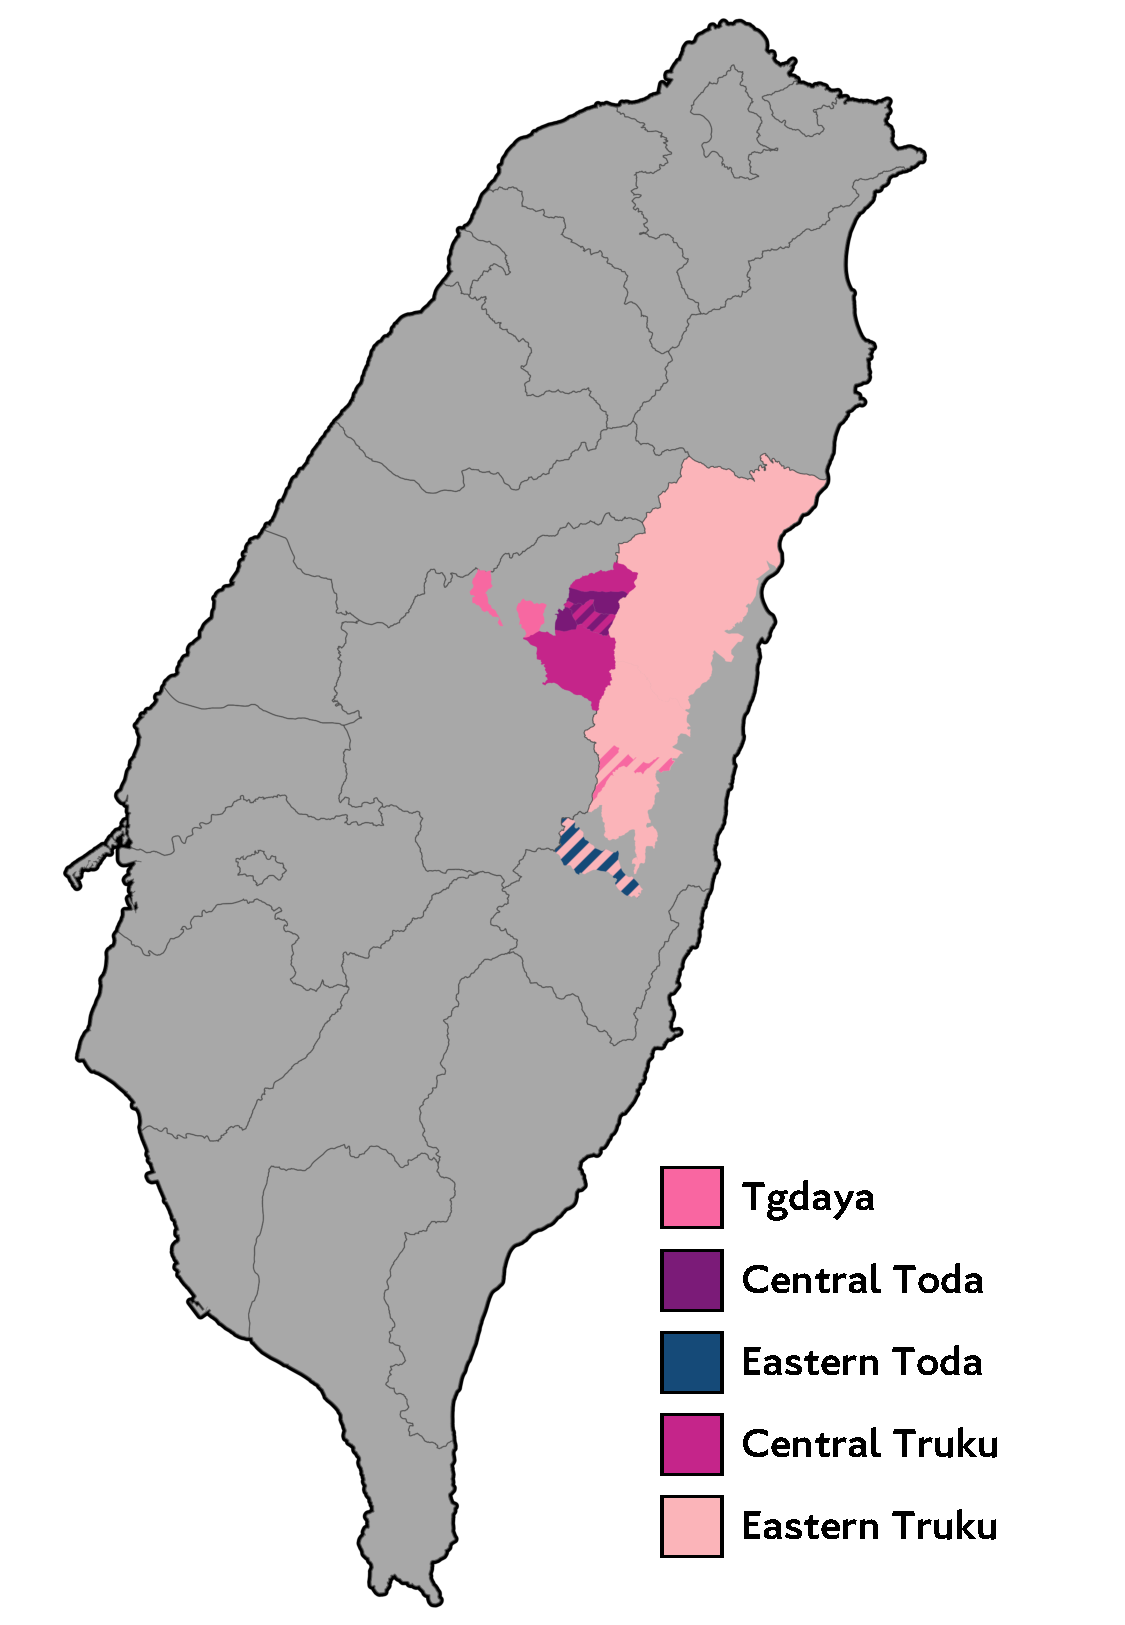
\includegraphics[width=1\linewidth]{img/dialectmap.pdf}
    \caption{Seediq speaking areas and dialectal distribution}
    \label{fig:dialectmap}
\end{figure}

\subsection{Tgdaya} \label{sec:tgintro}

Modern \acl{tg} dialect is distributed among the Gluban community (or Seryu, Chinese: 清流部落; Japanese: 川中島 \textit{Kawanakajima}) and Nakahara community (中原部落; 中原 \textit{Nakahara}) in Huzhu Village (互助村), and the Tongan community (or Bayke, 眉溪部落; 眉溪 \textit{Baikei}) in Nanfeng Village (南豐村). Both villages are in Ren'ai Township, Nantou County (南投縣仁愛鄉). 

Before the Musha Incident in 1930, the Tgdaya group in Nougougun, Taicyūsyū (臺中州能高郡, now Nantou County) comprised 12 communities, including: Paran, Tkanan, Qacuq, Gungu, Drodux, Suku, Mhebu, Truwan, Bwarung, Bkasan, Tongan, Sipo, marking the peak of the group. However, following the Musha Incident, a series of battles resulted in a significant loss of male warriors, with many women, children, and elderly individuals also choosing to end their lives. As a result, the population sharply declined (\cite{TengChian2023musha}).

After the Musha Incident, the Japanese authorities forcibly relocated six communities involved in the incident --- Mhebu, Truwan, Bwarung, Suku, Gungu, Drodux --- to what is now the Gluban community. Subsequently, in 1938, under the pretext of constructing the Bandai and Musha hydroelectric power plants (萬大と霧社発電所), three communities, Paran, Qacuq, and Tkanan, were relocated to the Nakahara (中原) between Gluban (川中島 \textit{Kawa\textbf{naka}jima}) and B'ala (眉原 \textit{Bai\textbf{bara}}, belongs to Atayal). Tongan and Sipo were later moved downstream not far from their original location in the 1950s and are now situated in the Tongan community (\cite{TengChian2023musha,iwanperin2005tongan}).

Some Tgdaya people migrated eastward from Tgdaya Truwan (Tək-daya-Tərowan in \cite{utsurikawaetal1935}) around the mid-19th century (\cite{liao1977Sedtheruy}). The Tgdaya people who migrated eastward are referred to as Pribaw or the Bokkui group (木瓜 bo̍k-kue `papaya' in Taiwanese; from Seediq \textit{bukuy} `back'). Their influence weakened due to raids from the eastern Taroko people. They currently reside in  Tngahan (Upper Mingli) community, Mingli Village, Wanrong Township, Hualien County (花蓮縣萬榮鄉明利村大加汗(上明利)部落), but their language usage and characteristics are not well-documented. Only few words were recorded in \textcite{tashiro1900easterntw}.

\subsection{Central Toda}

Modern \acl{cto} dialect is distributed in the Snuwil community (or Sakura, Gungu; Chinese: 史努櫻部落, formerly known as 春陽部落), Chunyang Village (春陽村); Toda community (都達部落 or formerly known as 平靜部落), and Ruku Daya community (平和部落) in the Toda village (都達村, formerly belonged to Chingying village (精英村)) of Ren'ai Township, Nantou County (南投縣仁愛鄉).

The current location of the Snuwil community was originally the Gungu community of the Tgdaya group. After the Musha Incident, the Tgdaya people left, and the Japanese authorities assigned this area to the Toda group. The residents of this community were originally from the Rucaw, Bngbung, Cka, Tnbarah, and Ruku Daya communities, who migrated to this location and formed the Snuwil community (\cite{Yap2011, Yap_ongoing_gaoshan}).

The remaining residents of Rucaw, Bngbung, Cka, and Tnbarah merged to form the Toda community, which continues to exist today. The remaining residents of Ruku Daya stayed in the local area, and after the World War II, some of the displaced residents returned to live there (\cite{Yap2011} and my field notes).

\subsection{Eastern Toda} \label{sec:etointro}

The Toda people who migrated eastward are known by different names, such as Tawsa, Tawsay, Tuda, etc. Some of them assimilated into the Klesan Atayal group (泰雅族南澳群) and switched to speak different variants of Yilan Creole (\cite{liao1977Sedtheruy,chienandsanada2010Ch}), whereas others gradually moved southward to their current location in Tawsa (or Tawsay) community, Lishan Village, Chuohsi Township, Hualien County (花蓮縣卓溪鄉立山村山里部落). 

The Toda group who migrated eastward, believes they originated from Tawsa-Truwan, approximately in the present-day Toda village area (南投縣仁愛鄉都達村). The migration path passed through areas such as today's Sqoyaw community of Atayal (環山部落, Seediq: Sqawraw), in Pingdeng village, Heping District, Taichung City (臺中市和平區平等里). There is a certain degree of similarity in clothing and accessories, with more diverse colors in female attire compared to other Seediq groups, including elements of purple, pink, and others.

There are some linguistic records of their language. \textcite{lee2012tawsa} introduces its phonological system and vocabulary, she shows that the has features of Toda but it is also influenced by Truku, making it a contact-induced dialect. 

\subsection{Central Truku}

Modern Central Truku dialect is used by four communities, all located in Ren'ai Township, Nantou County: Bwarung community (廬山部落) in Chingying Village (精英村); Truwan community (德魯灣部落, formerly known as 平生部落) and Sadu community (沙都部落, formerly known as 靜觀部落) in Truku Village (德鹿谷村, formerly known as Hecuo Village (合作村)); Pulan community (or Inago; 松林部落) in Chin'ai Village (親愛村).

Central Truku originally developed into five communities, including Truwan (Truku-Truwan), Sadu, Busig Ska, Busig Daya, and Brayaw. After the Musha Incident in 1930, the Japanese authorities first relocated some residents from communities other than Brayaw to where is now Pulan (Inago). Subsequently, the entire Brayaw community and some residents from other communities were moved to the Bwarung community, originally belonging to Tgdaya. The remaining residents of Truwan, Sadu, Busig Ska, and Busig Daya merged to form the Truku community. After World War II, it further divided back into Truwan and Sadu (\cite{Yap2011,Yap_ongoing_gaoshan}).

\subsection{Eastern Truku}

The Truku people who migrated to the Hualien area developed a total of 28 communities. Using a more inclusive calculation, the number can reach approximately 100, as mentioned by \textcite{liao1978Sedtheruy}. Due to space constraints, the complete list is not provided here. 

\textcite{liao1977Sedtheruy} suggests that this group originated from Truku-Truwan (near present-day Truwan and Sadu, located in Truku Village, Ren'ai Township, Nantou County), and they first established the Tpuqu community before starting to disperse. According to historical records and oral history, \textcite[200]{liao1978Sedtheruy} speculates that these communities arrived in the eastern region around or earlier than the mid-18th century.

After centuries of separation, this group of people developed a strong ethnic identity and urged independence from the Atayal Nation to form the Truku Nation in 2004. They refer to their ethnolect as ``Kari Truku (太魯閣語)''.

\section{Research questions and goals}

As mentioned earlier, there is currently a lack of comprehensive comparisons of Seediq dialects and reconstruction of \acl{psed} in academic research. My recent studies highlight the necessity of reconstructing \acl{psed} for understanding both the internal relationships of Seediq and those at a higher level (Atayalic). Additionally, there is no literature found that discusses the subgrouping and internal relationships of Seediq dialects based on a top-down approach. Most literature either focuses on superficial dialectal differences or employs criteria such as impression and mutual intelligibility for subgrouping (relevant discussions will be presented in Section \ref{sec:subgrouping_lit}). Furthermore, the influence of other Formosan languages on the development of Seediq has been less addressed in past literature.

Based on the identified research gaps, this thesis sets three main goals to address the aforementioned deficiencies: (1) Reconstruct the phonological system of \acl{psed} and conduct a preliminary exploration of its morphosyntactic system, (2) Investigate the subgrouping of Seediq dialects based on the reconstruction of \acl{psed}, and (3) Examine the contact relationships between Seediq and other Formosan languages.


\section{Methodology}\label{sec:methodology}

\subsection{The Comparative Method --- for bottom-up reconstruction and subgrouping}

This paper mainly employs the Comparative Method, a fundamental tool in historical linguistics, for the purpose of reconstructing Proto-Seediq and of subgrouping Seediq dialects. The Comparative Method is a systematic approach that involves several essential steps in order to uncover linguistic relationships and reconstruct ancestral languages (\cite{fox1995linguistic}).

The first step in this process is the collection of words from different Seediq dialects. By comparing these words, I aim to identify cognates, which are words that are similar or same in both form and meaning. The similar words among dialects also have to show regular sound correspondences in basic vocabulary. In addition, it is necessary to exclude the possibilities of ``chance'', ``universals'', and ``borrowing''. Cognates provide valuable evidence for language comparison and reconstruction.

Once cognates are identified, the next step involves setting up sound correspondences. Sound correspondences are regular patterns observed across cognate words. I will group these correspondence sets together based on their phonetic similarity. 

The third step employs a bottom-up reconstruction of protophonemes, which are the phonemes believed to have existed in the proto-language. In the process of reconstructing phonemes of a proto-language, careful attention must be given to the directionality of sound changes. Two fundamental reconstruction principles must be taken, as pointed out by \textcite[85]{crowley2010introduction}. Firstly, the sound change should be plausible and natural in language developments. Secondly, a reconstructed phoneme should minimize changes in both places and manners of articulation. By adhering to these principles, it becomes possible to reconstruct protophonemes for each corresponding group and identify consistent sound changes from the proto-language to its descendant languages.

Also, sound changes occurring from the proto-language to the descendant languages or dialects adhere to the principles of the Neogrammarian Hypothesis, alternatively recognized as the Regularity Hypothesis. According to this notion, sound changes follow a strict rule without any exceptions (\cite{brugmann1878morphologische}). In essence, a sound change is anticipated to be universally applied to all forms under defined conditions in a language or dialect. Irregular cases are typically observed solely in loanwords, sporadic sound changes, and accidental possibilities. For the phoneme inventory in the proto-language, we also expect it to be a balanced system. 

Using the protophonemes as a guide, I will also reconstruct the lexicon of \acl{psed}. By applying the sound correspondences and protophonemes to the cognate words, they can infer the likely forms of words in \acl{psed}. This step enables the reconstruction of a substantial portion of the lexicon.

Finally, the Comparative Method allows for the determination of subgrouping within the Seediq language. The subgrouping hypothesis in this paper is carried out based on the following criteria: (1) The primary method of subgrouping involves the use of exclusively shared innovations to form a subgroup, while shared retentions must not be employed as subgrouping criteria. \aikai{(2) Sporadic or rare sound changes are preferred over common ones as subgrouping criteria, as common sound changes might occur independently in closely related languages, representing a phenomenon known as ``drift'' or ``convergence among genetically related languages'', such as the ``Umlaut'' phenomenon in West-Germanic languages (\cite[47--48]{greenberg1957subgroupings}). (3) Phonological evidence includes conditioned shared sound changes, unique mergers, and more. (4) The lexical evidence referred to in this paper includes categories like lexical innovations, sporadic sound changes or segment replacements within words, and others. (cite Sapir for drift; 看廖老師 note)}

The paper will simultaneously consider the various aforementioned types of evidence as the basis for subgrouping, as situations might arise where a combination of two or more types of evidence is needed for judgment. These subgroups represent distinct historical stages or divisions within the Seediq language.

Overall, the application of the Comparative Method in this study of Seediq dialects involves collecting data, identifying cognates, establishing sound correspondences, reconstructing protophonemes and the lexicon, and determining subgroups. By following these steps, we are able to gain valuable insights into the historical development and relationships within the Seediq language, contributing to our understanding of its linguistic evolution.

\subsection{Top-down reconstruction method}

\aikai{The top-down reconstruction method is also known as ``inverted reconstruction'' (\cites[512--16]{hockett1958course}[346]{anttila1972introduction}).}

\aikai{For example, consider a language family shown in Figure \ref{fig:topdown}. We reconstruct proto-language *Y by comparing languages A and B, and proto-language *Z by comparing languages C and D. Proto-language *X is then reconstructed from *Y and *Z. However, evidence for the forms of *Y and *Z is not only found in the languages they originate from but also in *X. Once we've reconstructed the relevant forms of *X based on *Z and other languages, we can use these forms to reconstruct the forms of *Y from above (\cite[88]{fox1995linguistic}). }

\begin{figure}[H]
    \centering
           \begin{forest}
           for tree={l sep=5em, s sep=6em, inner sep=0, anchor=north, parent anchor=south, child anchor=north}
            [*X
                [*Y
                    [A]
                    [B]
                ]
                [*Z
                    [C]
                    [D]
                ]
            ]
            \end{forest}
        \caption{An assumed language family as an example for top-down reconstruction}
        \label{fig:topdown}
    \end{figure}

\aikai{In this paper, some of the reconstruction of \acl{psed} lexical forms is primarily guided by such a method. At times, modern Seediq dialects may exhibit two or more competing forms for a given word among them. In such cases, external evidence from \acl{pan} can assist in determining the \acl{psed} form. }

\aikai{However, considering that Atayalic languages often display numerous lexical innovations, it is frequently challenging to find evidence directly from \acl{pan}. Therefore, this paper employs a methodology which is similar to that of \textcite[187--88]{goderich2020phd} for the reconstruction of certain forms. If \acl{psed} has two candidates *a and *b for a specific lexical item, and if corresponding forms *b' or b'' exist in \acl{pata} or Atayal dialects, I will choose *b for the reconstruction in \acl{psed}. Relevant cases will be discussed in Section 6.2. }

\aikai{Certainly, in cases where a particular form appears in only one dialect, lacks agreement among the majority of dialects, or its meaning aligns with the characteristics of loanwords (such as expressing a highly specific meaning), the possibility of borrowing must be considered. Given that the Atayalic subbranch only contains two languages, the risk of circular reasoning is difficult to entirely avoid at this stage. I can only endeavor to eliminate instances fitting the aforementioned criteria as much as possible. To address this issue more effectively, a broader comparison of various Seediq and Atayal dialects, as well as an exploration of historical contact relationships between the two distinct language branches, may be necessary.}


\section{Data sources}
\lipsum[1-3]

\section{Orthographic conventions}

I apply the orthographic conventions in the paper in order to make an easier comparison of Seediq dialects. In general, the symbol used will be the same as those in the International Phonetic Alphabet (IPA), but there are still some exceptions. The conventions are shown in Table \ref{tab:orth}, and the current orthographic systems (MOE/CIP) that is used by the Seediq and Truku peoples are also listed for reference.\footnote{MOE and CIP are Abbreviations for Ministry of Education and Council of Indigenous Peoples of Taiwan, respectively.} 

\begin{table}[!htbp]
\centering
\caption{Orthographic conventions}
\label{tab:orth}
\begin{tabular}{lll|lll}
\hline
This thesis & MOE/CIP & IPA    & This thesis & MOE/CIP                   & IPA   \\ \hline
p          & p       & [p]    & r          & r                         & [ɾ]   \\
t          & t       & [t]    & l          & l                         & [l\~{ }ɮ] \\
k          & k       & [k]    & w          & w                         & [w]   \\
q          & q       & [q]    & y          & y                         & [j]   \\
b          & b       & [b]    & a          & a                         & [a]   \\
d          & d       & [d]    & i          & i                         & [i]   \\
g          & g       & [g\~{ }ɣ]  & u      & u                         & [u]   \\
c          & c       & [ʦ\~{ }ʨ]   & e     & e (\ac{tg})                  & [e]   \\
ɟ          & j       & [ɟ\~{ }ʥ] & ey      & ey (\ac{cto}, \ac{ctr}, \ac{etr})   & [ej]  \\
s          & s       & [s]    & ay         & ay (\ac{cto}, \ac{eto}, \ac{ctr}, \ac{etr})  & [aj]      \\
x          & x       & [x]    & o          & o (\ac{tg})                  & [o]   \\
h          & h       & [ħ]    & ow         & o/ow (\ac{cto}, \ac{ctr}, \ac{etr}) & [ow]  \\
m          & m       & [m]    & aw         & aw (\ac{cto}, \ac{eto}, \ac{ctr}, \ac{etr})                         & [aw]      \\
n          & n       & [n]    & ə          & ∅/e (\ac{cto}, \ac{eto}, \ac{ctr}, \ac{etr})    & [ə]   \\
ŋ          & ng      & [ŋ]    &            &                           &       \\ \hline
\end{tabular}
\end{table}

The symbol \textit{g} represents voiced velar stop or fricative [g\~{ }ɣ], as there are variations across different dialects. The symbols c and ɟ respectively denote [ʦ\~{ }ʨ] and [ɟ\~{ }ʥ]. In \acl{tg} and \acl{cto}, \textit{c} is phonemic, while \textit{c}/\textit{ɟ} in \acl{eto}, \acl{ctr}, and \acl{etr} represents palatalized allophones of /t/ and /d/. As for \textit{h}, it represents the voiceless pharyngeal fricative [ħ]. However, in certain (sub-)dialects or among speakers, it is also pronounced as a glottal [h]. Nevertheless, [ħ] is generally considered a more conservative pronunciation.

In the standard orthography, the velar nasal /ŋ/ is typically expressed as \textit{ng}, but for the purposes of this thesis, it will be designated with the IPA symbol \textit{ŋ}. The symbol \textit{r} represents the voiced alveolar tap [ɾ]. As the sole rhotic sound in this language, this sound may have other variations, but they do not significantly impact the phoneme inventories of different dialects or the reconstruction of \acl{psed}. \textit{l} represents the voiced alveolar/dental lateral (or lateral fricative) [l\~{ }ɮ], and \textit{y} denotes the voiced palatal approximant (``glide'') [j].

There is an issue about the ``neutralized'' (or reduced) vowel in prepenultimate syllables. In general, any kinds of vowel reduced into [u] (\ac{tg})/[ə] (non-\ac{tg}) in this specific environment. Since the vowel quality is predictable, it is omitted in the MOE/CIP system. For example, \textit{dtnqlian} (\ac{tg}) `a group of slaves' is pronounced as [dutunuquli(j)an]. In this paper, the ``omitted'' vowel in the MOE/CIP system will be transcribed based on the phonological system of each dialect. 

For the *e [ə] used in Blust's reconstruction of \acl{pan} (\cite{ACD}), this thesis will directly use *ə as the corresponding symbol. 

Modern languages (including Seediq and other languages) or languages with written records are marked in italics in this thesis. Reconstructed forms are marked with a single asterisk (*), and double asterisks (**) are used for the following categories: (1) forms of Pre-Proto-X, (2) intermediate stages in sound change processes, and (3) other hypothetical/expected forms that are unattested.

\section{Outline of the thesis}

This thesis is organized as follows: Chapter \ref{ch2} provides a literature review on three aspects related to the Seediq language, including external relationships, internal relationships, and relevant anthropological studies. Chapter \ref{ch3} introduces the phonological systems of modern Seediq dialects, encompassing phoneme inventories, phonotactics, and phonological rules. Chapter \ref{ch4}, based on the synchronic phonologies presented in Chapter 3, focuses on the reconstruction of the phonological system of \acl{psed}. This reconstruction extends to aspects such as lexicon, morphosyntax, and more. Chapter \ref{ch5} explores the proposed subgrouping of Seediq dialects and presents relevant evidence. Chapter \ref{ch6} discusses external relationships, including the development from \acl{pan} to \acl{psed}, language contact, and the insights that \acl{psed} provides for the reconstruction of \acl{paic}. Chapter \ref{ch7} serves as the conclusion, summarizing the thesis and discussing remaining issues and potential future research directions.
\chapter{Literature review}
\lipsum[1]

\section{The position of Seediq in the Austronesian family} \label{sec:position}
\lipsum[1-5]

\section{Internal relationships of Seediq dialects}
\lipsum[1-5]

\section{Relevant anthropology studies}
\lipsum[1-5]

\section{Interim summary}
\lipsum[1]

\chapter{Phonologies of Seediq dialects}\label{ch3}
This chapter provides the synchronic phonological sketches of five Seediq dialects: \acl{tg}, \acl{cto}, \acl{eto}, \acl{ctr}, and \acl{etr}. Section \ref{sec:3.1} discusses the phoneme inventories and phonotactics of all the five dialects. In section \ref{sec:3.2}, different kinds of alternations are discussed, especially those related to morphophonology.

\section{Phoneme inventories and phonotactics} \label{sec:3.1}

This section introduces the phoneme inventories and phonotactics of various Seediq dialects. While the consonant inventories of Seediq dialects are similar, there are still differences; however, the vowels, particularly in \acl{tg}, exhibit more distinctiveness.

Regarding phonotactics, there is a high level of consistency among dialects in terms of constraints on the occurrence of some sounds in certain positions. Stress placement is non-phonemic, with the majority of cases regularly falling on the penultimate syllable, while Central Toda exhibits a stress shift when the penultimate vowel is schwa /ə/ (See Section \ref{sec:cto_phonotactics}).

\subsection{Tgdaya phonology}

\subsubsection{Tgdaya consonant inventory}

\acl{tg} has the largest number of consonants among all dialects. The \acl{tg} dialect has eighteen consonants, including seven stops \textit{p, t, k, q, b, d, g}, one affricate \textit{c} [ʦ], three fricatives \textit{s, x, h} [ħ], three nasals \textit{m, n, ŋ}, one lateral \textit{l}, one tap \textit{r} [ɾ], and two glides \textit{w, y} [j]. Table \ref{tab:tgC} shows the consonant inventory of \acl{tg}.

\begin{table}[!htbp]
\centering
\caption{Tgdaya consonant inventory\\}
\label{tab:tgC}
\begin{tabular}{l|ll|ll|ll|ll|ll|ll}
\hline
                    & \multicolumn{2}{c|}{Bilabial} & \multicolumn{2}{c|}{Dental/Alveolar} & \multicolumn{2}{c|}{Palatal} & \multicolumn{2}{c|}{Velar} & \multicolumn{2}{c|}{Uvular} & \multicolumn{2}{c}{Pharyngeal} \\ \hline
Stop                & p            & b           & t               & d               &             &               & k          & g          & q            &            &                 &              \\
Fricative           &               &              & s               &                  &             &               & x          &             &               &            & h [ħ]             &              \\
Affricate           &               &              & c [ʦ]              &                  &             &               &             &             &               &            &                 &              \\
Nasal               &               & m           &                  & n               &             &               &             & ŋ          &               &            &                 &              \\
Lateral &               &              &                  & l               &             &               &             &             &               &            &                 &              \\
Tap                 &               &              &                  & r [ɾ]              &             &               &             &             &               &            &                 &              \\
Glide               &               & w           &                  &                  &             & y [j]           &             &             &               &            &                 &              \\ \hline
\end{tabular}
\end{table}

<h> is realized as a pharyngeal [ħ] by more conservative speakers; on the contrary, other speakers pronounce it as a glottal [h] (also by some elder speakers). Further investigation is needed to determine whether this is influenced by age or other factors (such as societal ones). Additionally, careful phonetic studies are required. But phonologically, the realizations of this phoneme do not change the categorical properties, and it is clearly distinct from velar fricative /x/.

<c> /ʦ/ and <s> always palatalize to [ʨ] and [ɕ] before the high front vowel /i/, and whether it occurs in other environments depends on the speaker. Common environments include: (1) \textit{i}\_\#, and (2) \_\textit{e}. For example, \textit{madis} [madiɕ] `to bring \acs{av}', \textit{cebu} [ʨebu] `to shoot'. 

<l> is a lateral sound, but in the realization of some speakers, it may exhibit slight frication. However, due to the lack of noise, it does not reach the level of [ɮ].

<r> is usually pronounced as an alveolar (or retracted) tap [ɾ\~{}ɾ̠] or a retroflex flap [ɽ]. However, as the only rhotic sound, there may be even more variations, such as approximants [ɹ\~{}ɻ] or even (rarely) a trill [r].

Regarding the glottal stop [ʔ], \textcite{yang1976sedpho} argues that it lacks phonemic status and that the phonetic realization of [ʔ] and ∅ can be in free variation. Conversely, \textcite{holmer1996parametric} classifies the glottal stop as the phoneme /ʔ/, but without further explanation. \textcite{Sung2018Sedgrammar} does not consider it as a phoneme and also does not provide an explanation. Since the occurrence of the glottal stop [ʔ] can be predicted and there is no phonemic distinction from ∅, I adopt Yang's view and do not consider the glottal stop as a phoneme in this thesis.

\subsubsection{Tgdaya vowel inventory}

\acl{tg} has five monophthongs: \textit{a, i, e, u, o}, as shown in Table \ref{tab:tgV}. In addition to monophthongs, \acl{tg} has a diphthong -\textit{uy} [uj]. 

\begin{table}[!htbp]
\centering
\caption{Tgdaya vowel inventory}
\label{tab:tgV}
\begin{tabular}{llll}
\hline
     & Front & Central & Back \\ \hline
High &  i    &         &  u   \\
Mid  &  e    &         &  o   \\
Low  &       &  a      &      \\ \hline
\end{tabular}
\end{table}

In Tgdaya, vowel length is not distinguished. If a sequence of two identical vowels is seen, the two vowels actually belong to two separate syllables, as in \textit{haan} [ħa.an] `to go \acs{lv}'.

\subsubsection{Tgdaya phonotactics}

Table \ref{tab:sy_ty_tg} displays the syllable types of \acl{tg}, listing the syllable types covered in slower and deliberate speech. In everyday and faster speech, other types may occur, which will be briefly introduced later on. Please note that the symbol C in the coda position includes all consonants except for glides, while G represents the two glides \textit{w} and \textit{y}. In the onset position, there is no distinction, and all non-vowel sounds are unified under C. This convention applies to other parts of the thesis as well.

\begin{table}[!htbp]
\centering
\caption{Syllable types in Tgdaya}
\label{tab:sy_ty_tg}
\begin{tabular}{lllllll}
\hline
Syll. type & \multicolumn{2}{l}{Prepenultimate} & \multicolumn{2}{l}{Penultimate} & \multicolumn{2}{l}{Final}                \\ \hline
V             & ---              &                 & \textbf{i}.ma            & `who'         & sa.\textbf{i}        & `to go.\acs{imp} \acs{pv}' \\
VC            & ---              &                 & ---             &               & sa.\textbf{un}       & `to go \acs{pv}'           \\
VG            & ---              &                 & ---             &               & (not found) &                            \\
CV            & \textbf{qu}.si.ya         & `water'         & qu.\textbf{si}.ya        & `water'       & qu.si.\textbf{ya}    & `water'                    \\
CVC           & ---              &                 & ---             &               & ba.\textbf{raq}      & `lungs'                    \\
CVG           & ---              &                 & ---             &               & lu.\textbf{buy}      & `bag'                     \\ \hline
\end{tabular}
\end{table}

CV is the only syllable type allowed to appear in the prepenultimate position. Onsetless V will be deleted by a universal phonological rule, as seen in \textit{eyah} /ejaħ/ `to come' and \textit{yah-an} /ejaħ/ + /an/ `to come \acs{lv}'. In the penultimate position, only V and CV structures are allowed to appear.

In the final position, \acl{tg} can at least have five structures: V, VC, CV, CVC, and CVG, with fewer restrictions. While the VC structure is speculated to be possible, examples may be relatively rare and harder to find. In other dialects, there is \textit{dəmuuy} `to hold in fist \acs{av}', but irregularly corresponds to \textit{dumoi} in \acl{tg}.

In faster speech, two other syllable structures that are commonly found and are both related to nasals can occur: CVN and N̩. When the nasal consonant is followed by a homorganic consonant, syncope occurs between the nasal and the following consonant. If there is a preceding syllable before the nasal consonant, the nasal consonant becomes the coda of the preceding syllable. If there is no preceding syllable, the nasal sound becomes syllabic. These syllable structures' occurrences can be considered surface phenomena. For example, /tunusapaħ/ → [\textbf{tun}.sa.paħ] `family', and /mupitu/ → [\textbf{m̩}.pi.tu] `seven'. These variations may differ depending on individuals or subdialects.

Some sounds in \acl{tg} also have positional restrictions, some of them are categorical. For instance, voiced stops /b/, /d/, /g/ do not occur in word-final position. Labial consonants /p/ (including /b/) and /m/ are also not found in such position. 

The phoneme /x/ only appears at the word-initial position in the word \textit{\textbf{x}iluy} `iron', with around ten more examples found word-medially, but it is more common in word-final position.

In a significant portion of speakers, both liquids /l/ and <r> /ɾ/ merge with /n/ in word-final position, respectively. More conservative speakers maintain the distinctions, but generally, the merger of /l/ and /n/ in word-final position is more common than that of <r> /ɾ/ and /n/. Speakers of \acl{tg} who retain the word-final <r> often realize it as an approximant [ɹ\~{}ɻ], unlike the tap/flap in word-initial and word-medial positions. Of course, there may be more variants because, as mentioned earlier, this is the only rhotic sound in the language.

The word-final glide /w/ and <y> /j/ can only occur with /u/, as in \textit{el\textbf{uw}} `road' and \textit{bab\textbf{uy}} `pig', while in other positions, there are no restrictions.

The mid vowels /e/ and /o/ primarily serve as the nucleus of open syllables due to the historical developments (see Section \ref{sec:psedV}). However, with language development or analogical changes, there may be extremely rare exceptions, such as the occurrence of \textit{muuyas} \~{} \textit{muu\textbf{wes}} /muujas/ `to sing; to study \acs{av}' in casual speech.

In \acl{tg}, there is a rule of neutralization of prepenultimate vowels, with the neutral vowel being /u/. This means that, in general, vowel distinctions only occur in penultimate and final syllables, while the vowels in prepenultimate syllables are neutralized to [u]. However, when the onset of the penultimate syllable is <h> /ħ/ or has no onset (i.e., the onset is ∅), the neutralized vowel of the antipenultimate syllable is assimilated to be the same as the penultimate syllable, as in \textit{m\textbf{e}h\textbf{e}diq} [m\textbf{e}.ħ\textbf{e}.diq] `to give way \acs{av}' and \textit{s\textbf{ii}mah} [s\textbf{i}.\textbf{i}.maħ] `to drink \acs{cv}'. However, there are exceptions, such as \textit{m\textbf{u}h\textbf{u}hediq} [m\textbf{u}.ħ\textbf{u}.ħe.diq] `to give way to each other' instead of *[m\textbf{e}.ħ\textbf{e}.ħe.diq], possibly indicating that vowel features tend to spread only once. Further synchronic phonological analysis is needed to explore this phenomenon.


\subsection{Central Toda phonology}

\subsubsection{Central Toda consonant inventory}

The \acl{cto} dialect has seventeen consonant, including six stops \textit{p, t, k, q, b, d}, one affricate \textit{c} [ʦ], three fricatives \textit{s, x, h} [ħ], three nasals \textit{m, n, ŋ}, one lateral \textit{l}, one tap \textit{r} [ɾ], and two glides \textit{w, y} [j]; the inventory is as given in Table \ref{tab:ctoC}.

\begin{table}[!htbp]
\centering
\caption{Central Toda consonant inventory}
\label{tab:ctoC}
\begin{tabular}{l|ll|ll|ll|ll|ll|ll}
\hline
                    & \multicolumn{2}{c|}{Bilabial} & \multicolumn{2}{c|}{Dental/Alveolar} & \multicolumn{2}{c|}{Palatal} & \multicolumn{2}{c|}{Velar} & \multicolumn{2}{c|}{Uvular} & \multicolumn{2}{c}{Pharyngeal} \\ \hline
Stop                & p            & b           & t               & d               &             &               & k          &            & q            &            &                 &              \\
Fricative           &               &              & s               &                  &             &               & x          &             &               &            & h [ħ]             &              \\
Affricate           &               &              & c [ʦ]              &                  &             &               &             &             &               &            &                 &              \\
Nasal               &               & m           &                  & n               &             &               &             & ŋ          &               &            &                 &              \\
Lateral &               &              &                  & l               &             &               &             &             &               &            &                 &              \\
Tap                 &               &              &                  & r [ɾ]              &             &               &             &             &               &            &                 &              \\
Glide               &               & w           &                  &                  &             & y [j]           &             &             &               &            &                 &              \\ \hline
\end{tabular}
\end{table}

\acl{cto} lacks the consonant <g> (/g/ or /ɣ/). Apart from this, the consonant inventory is the same as the one in \acl{tg}. 

<s> and <c> /ʦ/ also palatalize to [ɕ] and [ʨ] before the high front vowel /i/, but do not occur in other environments. The fricative <h> can be either pharyngeal [ħ] or glottal [h]. 

The lateral <l> also exhibits slight frication, similar to Tgdaya. The rhotic <r> can also be realized as an alveolar (or retracted) tap [ɾ\~{}ɾ̠] or a retroflex flap [ɽ], and in word-final position, it is also a tap/flap with a release, not an approximant.

\subsubsection{Central Toda vowel inventory}

\acl{cto} has four monophthongs: \textit{a, i, u, ə}, as shown in Table \ref{tab:ctoV}.

\begin{table}[!htbp]
\centering
\caption{Central Toda vowel inventory}
\label{tab:ctoV}
\begin{tabular}{llll}
\hline
     & Front & Central & Back \\ \hline
High &  i    &         &  u   \\
Mid  &       &  ə      &      \\
Low  &       &  a      &      \\ \hline
\end{tabular}
\end{table}

Apart from monophthongs, \acl{cto} has three phonemic diphthongs: /aw/, /aj/, and /uj/. The diphthong /aw/ has two allophones: [ow] and [aw]. [ow] appears in word-medial positions, as in \textit{dowriq} `eye', while [aw] occurs in word-final positions, as in \textit{babaw} `above; on top of'. The two allophones are in complementary distribution. The same situation also occurs with <ey> [ej] and <ay> [aj], where the phoneme /aj/ is the allophone in word-medial and word-final positions, as in \textit{meytaq} `to stab \acs{av}' and \textit{balay} `true; correct'. However, <uy> /uj/ can only occur in word-final position.

\subsubsection{Central Toda phonotactics} \label{sec:cto_phonotactics}

The syllable types of \acl{cto} are shown in Table \ref{tab:sy_ty_cto}. 

\begin{table}[!htbp]
\centering
\caption{Syllable types in Central Toda}
\label{tab:sy_ty_cto}
\begin{tabular}{lllllll}
\hline
Syll. type & \multicolumn{2}{l}{Prepenultimate} & \multicolumn{2}{l}{Penultimate} & \multicolumn{2}{l}{Final}                \\ \hline
V             & \textbf{u}.ci.luŋ & `lake; sea'    & \textbf{i}.ma            & `who'         & sa.\textbf{i}        & `to go.\acs{imp} \acs{pv}' \\
VC            & ---              &                 & ---             &               & sa.\textbf{un}       & `to go \acs{pv}'           \\
VG            & ---              &                 & \textbf{ow}.raw   & `k.o. bamboo' & də.mu.\textbf{uy} &  `to hold \acs{av}'        \\
CV            & \textbf{qə}.si.ya         & `water'         & qə.\textbf{si}.ya        & `water'       & qə.si.\textbf{ya}    & `water'                    \\
CVC           & ---              &                 & ---             &               & ba.\textbf{raq}      & `lungs'                    \\
CVG           & ---              &                 & \textbf{dow}.riq     & `eye'    & lu.\textbf{buy}      & `bag'                     \\ \hline
\end{tabular}
\end{table}

% 補說明

% 補語音限制

\subsection{Eastern Toda phonology}

The \acl{eto} dialect has sixteen consonant, including six stops \textit{p, t, k, q, b, d}, three fricatives \textit{s, x, h} [ħ], three nasals \textit{m, n, ŋ}, one lateral \textit{l}, one tap \textit{r} [ɾ], and two glides \textit{w, y} [j]; the inventory is as given in Table \ref{tab:etoC}.

\begin{table}[!htbp]
\centering
\caption{Eastern Toda consonant inventory}
\label{tab:etoC}
\begin{tabular}{l|ll|ll|ll|ll|ll|ll}
\hline
                    & \multicolumn{2}{c|}{Bilabial} & \multicolumn{2}{c|}{Dental/Alveolar} & \multicolumn{2}{c|}{Palatal} & \multicolumn{2}{c|}{Velar} & \multicolumn{2}{c|}{Uvular} & \multicolumn{2}{c}{Pharyngeal} \\ \hline
Stop                & p            & b           & t \quad\quad\quad          & d               &             &               & k          &            & q            &            &                 &              \\
Fricative           &               &              & s               &                  &             &               & x          &             &               &            & h [ħ]             &              \\
Nasal               &               & m           &                  & n               &             &               &             & ŋ          &               &            &                 &              \\
Lateral &               &              &                  & l               &             &               &             &             &               &            &                 &              \\
Tap                 &               &              &                  & r [ɾ]              &             &               &             &             &               &            &                 &              \\
Glide               &               & w           &                  &                  &             & y [j]           &             &             &               &            &                 &              \\ \hline
\end{tabular}
\end{table}

% 補說明

\subsubsection{Eastern Toda consonant inventory}

\acl{eto} has four monophthongs: \textit{a, i, u, ə}, as shown in Table \ref{tab:etoV}.

\begin{table}[!htbp]
\centering
\caption{Eastern Toda vowel inventory}
\label{tab:etoV}
\begin{tabular}{llll}
\hline
     & Front & Central & Back \\ \hline
High &  i    &         &  u   \\
Mid  &       &  ə      &      \\
Low  &       &  a      &      \\ \hline
\end{tabular}
\end{table}

% 補雙元音、說明

\subsubsection{Eastern Toda vowel inventory}
\lipsum[1-3]

\subsubsection{Eastern Toda phonotactics}
\lipsum[1-3]

\subsection{Central and Eastern Truku phonologies}
\lipsum[1]

\subsubsection{Truku consonant inventory}
\lipsum[1-3]
\subsubsection{Truku vowel inventory}
\lipsum[1-3]
\subsubsection{Truku phonotactics}
\lipsum[1-3]

\section{Synchronic alternations} \label{sec:3.2}

In each Seediq dialect, there are some phonological alternations, often resulting from the interaction between position of the sounds and morphology. Interestingly, the patterns of alternations among dialects exhibit a considerable degree of consistency. Most alternating patterns can be traced back to \acl{psed}, implying that synchronic alternations can be viewed as remnants of the Proto-Seediq (See Section \ref{sec:psed_alter} for the alternations in \acl{psed}).

This section attempts to explore all alternations as comprehensively as possible. However, there may still be areas that are not fully developed, such as specific alternations in subdialects of certain villages. In this section, segments participating in alternations and currently under discussion will be bolded, while alternations that are not the immediate focus will not be highlighted prominently. 

\subsection{Vowel alternations}

\subsubsection{Prepenultimate vowel neutralizing}
\lipsum[1-3]

\subsubsection{Alternations of [ə]\~{}[u] or [e]\~{}[u]}
\lipsum[1-3]

\subsubsection{Alternations related to vowel hiatus}
\lipsum[1-3]

\subsubsection{Vowel coalescence}
\lipsum[1-3]

\subsubsection{Apharesis} %首音刪除
\lipsum[1-3]

\subsubsection{Syncope}
\lipsum[1-3]

\subsubsection{Vowel harmony}
\lipsum[1-3]

\subsubsection{Alternation between monophthongs and diphthongs}
\lipsum[1-3]

\subsection{Consonant alternations}

Consonantal alternations are highly correlated with the word-final position of the sound (with a few exceptions), often occurring when attaching suffixes due to no longer being in such position. However, sometimes a set of alternations may be related to more than one phonological rule, making classification challenging. Therefore, this section will provide separate explanations through direct examples and combine similar cases for discussion.

\subsubsection{Alternations between -\textit{d}/\textit{t}- and -\textit{c}}
\lipsum[1-3]

\subsubsection{Alternations between -\textit{b}/\textit{p}- and -\textit{k}}
\lipsum[1-3]

\subsubsection{Alternation between -\textit{m}- and -\textit{ŋ}}
\lipsum[1-3]

\subsubsection{Alternations related to -V\textit{g}- sequences}
\lipsum[1-3]

\subsubsection{Alternations between -\textit{l}/\textit{r}- and -\textit{n}}
\lipsum[1-3]

\subsubsection{Palatalization and affrication of alveolar stops before \textit{i} and \textit{y}}
\lipsum[1-3]






\section{Interim summary}
\lipsum[1-2]
%\chapter{Proto-Seediq phonology}\label{ch4}

In this chapter, I will first present the phoneme inventory of \acl{psed}. Subsequently, I will list out each reconstructed phoneme along with their reflexes and lexical examples in modern dialects. Please note that data from \acl{eto} is only presented when it is \textbf{crucial for reconstruction}. I will also show and explain irregular and/or inconsistent sound correspondences and discuss what proto-phonemes they should be reconstructed as. Additionally, the phonotactics of \acl{psed} and morphophonological alternations that can be reconstructed to the proto-language level will be addressed.

\section{Proto-Seediq phoneme inventory}

Table \ref{tab:psedC} shows the consonant inventory of \acl{psed}. There are 18 consonants in \acl{psed} based on my reconstruction, including:

\begin{enumerate}[label=(\roman*), itemsep=0pt, topsep=0pt]
    \item six stops: *p, *t, *k, *q, *b, *d
    \item one affricate: *c
    \item four fricatives: *s, *x, *h, *g
    \item three nasals: *m, *n, *ŋ
    \item two liquids: *l, *r
    \item two glides: *w, *y
\end{enumerate}

\begin{table}[!htbp]
\centering
\caption{Proto-Seediq consonant inventory}
\label{tab:psedC}
\begin{tabular}{l|ll|ll|ll|ll|ll|ll}
\hline
                    & \multicolumn{2}{c|}{Bilabial} & \multicolumn{2}{c|}{Dental/Alveolar} & \multicolumn{2}{c|}{Palatal} & \multicolumn{2}{c|}{Velar} & \multicolumn{2}{c|}{Uvular} & \multicolumn{2}{c}{Pharyngeal} \\ \hline
Stop                & *p            & *b           & *t  \quad\quad\quad             & *d               &             &               & *k          &           & *q            &            &                 &              \\
Affricate           &               &              & *c               &                  &             &               &             &             &               &            &                 &              \\
Fricative           &               &              & *s               &                  &             &               & *x          & *g         &               &            & *h              &              \\
Nasal               &               & *m           &                  & *n               &             &               &             & *ŋ          &               &            &                 &              \\
Lateral  &               &              &                  & *l               &             &               &             &             &               &            &                 &              \\
Tap/Flap                 &               &              &                  & *r               &             &               &             &             &               &            &                 &              \\
Glide               &               & *w           &                  &                  &             & *y            &             &             &               &            &                 &              \\ \hline
\end{tabular}
\end{table}

The vowel inventory of \acl{psed} is straightforward, as shown in Table \ref{tab:psedV}. There are four monophthongs in \acl{psed}, which are *a, *i, *u, and *ə. Note that mid vowels [e] and [o] cannot be found in \acl{psed}. There are three ``diphthongs'' (VG sequences) in \acl{psed}, including *ay, *aw, and *uy. 

\begin{table}[!htbp]
\centering
\caption{Proto-Seediq vowel inventory}
\label{tab:psedV}
\begin{tabular}{lcccccccc}
\cline{1-4} \cline{7-9}
     & Front & Central & Back &  &  & \multicolumn{3}{c}{``diphthongs''} \\ \cline{1-4} \cline{7-9}
High & *i    &         & *u   &  &  &            & *uy       &           \\
Mid  &       & *ə      &      &  &  &            &           &           \\
Low  &       & *a      &      &  &  & *ay        &           & *aw       \\ \cline{1-4} \cline{7-9}
\end{tabular}
\end{table}

\section{Reconstructed phonemes and their reflexes} \label{sec:psed_CandV}

This section reconstructs the proto-phonemes in \acl{psed} by comparing segments from words collected from modern dialects. Additionally, I demonstrates the reflexes of these reconstructed phonemes in modern dialects across different positions and environments (if applicable).

\subsection{Proto-Seediq consonants} \label{sec:psedC}

\subsubsection{Proto-Seediq obstruents}

Reflexes of \acl{psed} *p can be found in word-initial and medial positions in all dialects, as given in the reflexes of *pahuŋ `gallbladder' and *səpi `dream' in Table \ref{tab:psed_p}. However, no Seediq dialects have a word-final -\textit{p}, because there was a merger of word-final *-k and *-p as *-k from Proto-Atayalic to (Proto-)Seediq (\cite{li1981paic}). Li also points out that this merger is natural because [p] and [k] share the feature [+grave]. 

\begin{table}[!htbp]
\centering
\caption{Reflexes of \acl{psed} *p}
\label{tab:psed_p}
\begin{tabular}{lll}
\hline
           & *p-    & *-p-  \\ \hline
\acs{psed} & *\textbf{p}ahuŋ & *sə\textbf{p}i \\ \hdashline
\acs{tg}   & \textbf{p}ahuŋ  & se\textbf{p}i  \\
\acs{cto}  & \textbf{p}ahuŋ  & sə\textbf{p}i  \\
% \acs{eto}  &        &       \\
\acs{ctr}  & \textbf{p}ahuŋ  & sə\textbf{p}i  \\
\acs{etr}  & \textbf{p}ahuŋ  & sə\textbf{p}i  \\ \hline
Gloss      & `gallbladder'   & `dream'        \\ \hline
\end{tabular}
\end{table}

In suffixed forms of \acl{psed} words that contain a final *-k from the historical **-p, we can find the final consonant alternating between *k (in non-suffixed forms, like AV form and bare form) and *p (in suffixed forms such as PV form and LV form). Such as *miyu\textbf{k} `to blow (AV)' and *yu\textbf{p}un `to blow (PV)'. I will provide a more detailed description of the alternations in \acl{psed} in Section \ref{sec:psed_alter}.

Reflexes of \acl{psed} *t are relatively more complicated, as shown in Table \ref{tab:psed_t}. \acl{psed} *t is reflected as \textit{c} before \textit{i} in \acs{eto}, \acs{ctr}, and \acs{etr}. More precisely, *t underwent a palatalization and an affrication processes and changed to an affricate \textit{c} [ʨ] in this environment. The relevant examples can be found in the reflexes of *timu `salt' and *quti `feces' in above-mentioned dialects. 

\begin{table}[!htbp]
\centering
\caption{Reflexes of \acl{psed} *t}
\label{tab:psed_t}
\begin{tabular}{llllll}
\hline
           & *t-    & *t- /\_i & *-t-  & *-t- /\_i & *-t    \\ \hline
\acs{psed} & *\textbf{t}unux & *\textbf{t}imu    & *u\textbf{t}ux & *qu\textbf{t}i     & *səpat \\ \hdashline
\acs{tg}   & \textbf{t}unux  & \textbf{t}imu     & u\textbf{t}ux  & qu\textbf{t}i      & sepac  \\
\acs{cto}  & \textbf{t}unux  & \textbf{t}imu     & u\textbf{t}ux  & qu\textbf{t}i      & səpac  \\
\acs{eto}  &        & \textbf{c}imu&       &           &        \\
\acs{ctr}  & \textbf{t}unux  & \textbf{c}imu     & u\textbf{t}ux  & qu\textbf{c}i      & səpac  \\
\acs{etr}  & \textbf{t}unux  & \textbf{c}imu     & u\textbf{t}ux  & qu\textbf{c}i      & səpat  \\ \hline
Gloss      & `head' & `salt'   & `spirit' & `feces'  & `four' \\ \hline
\end{tabular}
\end{table}

In word-final position, \acl{psed} *t is reflected as \textit{c} [ʦ(ʰ)] in \acl{tg}, \acl{cto}, \acl{eto}, and \acl{ctr}. However, the final affrication seems to be optional and phonetic because the speakers do not release the final stops all the time, especially if there is another word following it. For example, \textit{sepac papak} `four legs' (\acs{tg}) can be pronounced as either [sepaʦʰ papakʰ] or [sepat̚ \ papakʰ]. 

In addition to the environments mentioned above, \acl{psed} *p is consistently reflected as /t/ in other positions, as seen in the reflexes of *tunux `head' and *utux `spirit' in Table \ref{tab:psed_t}.

\acl{psed} *k is reflected as /k/ in all positions in every dialect, as shown in the reflexes of *kari `language', *yaku `\textsc{1sg.nom}', and *papak `animal foot' in Table \ref{tab:psed_k}.

\begin{table}[!htbp]
\centering
\caption{Reflexes of \acl{psed} *k}
\label{tab:psed_k}
\begin{tabular}{llll}
\hline
           & *k-        & *-k-               & *-k           \\ \hline
\acs{psed} & *\textbf{k}ari      & *ya\textbf{k}u              & *papa\textbf{k}        \\ \hdashline
\acs{tg}   & \textbf{k}ari       & ya\textbf{k}u               & papa\textbf{k}         \\
\acs{cto}  & \textbf{k}ari       & ya\textbf{k}u               & papa\textbf{k}         \\
% \acs{eto}  &            &                    &               \\
\acs{ctr}  & \textbf{k}ari       & ya\textbf{k}u               & papa\textbf{k}         \\
\acs{etr}  & \textbf{k}ari       & ya\textbf{k}u               & papa\textbf{k}         \\ \hline
Gloss      & `language' & `\textsc{1sg.nom}' & `animal foot' \\ \hline
\end{tabular}
\end{table}

The voiceless uvular stop *q is also regular in all the Seediq dialects under study, and can be found in all positions, as seen in reflexes of *quyux `rain', *laqi `child', and *dawriq `eye' Table \ref{tab:psed_q}. \textcite{li1981paic} notes that \acl{paic} *q has shifted to an epiglottal (or pharyngealized glottal) stop /ʡ/ in Truwan Seediq. 

\begin{table}[!htbp]
\centering
\caption{Reflexes of \acl{psed} *q}
\label{tab:psed_q}
\begin{tabular}{llll}
\hline
           & *q-    & *-q-    & *-q     \\ \hline
\acs{psed} & *\textbf{q}uyux & *la\textbf{q}i   & *dawri\textbf{q}  \\ \hdashline
\acs{tg}   & \textbf{q}uyux  & la\textbf{q}i    & dori\textbf{q}   \\
\acs{cto}  & \textbf{q}uyux  & la\textbf{q}i    & dowri\textbf{q}   \\
% \acs{eto}  &        &         & dawri\textbf{q}  \\
\acs{ctr}  & \textbf{q}uyux  & la\textbf{q}i    & dowri\textbf{q}   \\
\acs{etr}  & \textbf{q}uyux  & la\textbf{q}i    & dowri\textbf{q}   \\ \hline
Gloss      & `rain' & `child' & `eye' \\ \hline
\end{tabular}
\end{table}

Reflexes of *b are generally regular in every dialect in the word-initial and medial positions, as shown in *birat `ear' and *ubal `fur; body hair' in Table \ref{tab:psed_b}. Like /p/, /b/ can not be found in word-final position in the modern dialects either. *-b merged with *-k word-finally, but the final consonant alternation can still be noticed between the AV forms and LV/PV forms, as in *məlu\textbf{k} `to close (AV)' and *lə\textbf{b}an `to close (LV)'. 

\begin{table}[!htbp]
\centering
\caption{Reflexes of \acl{psed} *b}
\label{tab:psed_b}
\begin{tabular}{lll}
\hline
           & *b-    & *-b-             \\ \hline
\acs{psed} & *\textbf{b}irat & *u\textbf{b}al            \\ \hdashline
\acs{tg}   & \textbf{b}irac  & u\textbf{b}an             \\
\acs{cto}  & \textbf{b}irac  & u\textbf{b}al             \\
% \acs{eto}  &        &                  \\
\acs{ctr}  & \textbf{b}irac  & u\textbf{b}al             \\
\acs{etr}  & \textbf{b}irat  & u\textbf{b}al             \\ \hline
Gloss      & `ear'  & `fur; body hair' \\ \hline
\end{tabular}
\end{table}

\acl{psed} *d is reflected as \textit{ɟ} [ɟ\~{ }ʥ] in \acl{eto}, \acl{ctr}, and \acl{etr} before \textit{i}, which parallels the development of \acl{psed} *t. In other environments, \acl{psed} *d is reflected as /d/ in all other word-initial and medial positions. Note that no word-final /d/ is found in any dialect. For reflexes of \acl{psed} *d, please refer to *dara `blood', *diyan `daytime', *rudan `old (person)', and *səədiq `human' in Table \ref{tab:psed_d}. 

\begin{table}[!htbp]
\centering
\caption{Reflexes of \acl{psed} *d}
\label{tab:psed_d}
\begin{tabular}{lllll}
\hline
           & *d-     & *d- /\_i  & *-d-           & *-d- /\_i       \\ \hline
\acs{psed} & *\textbf{d}ara   & *\textbf{d}iyan    & *ru\textbf{d}an         & *səə\textbf{d}iq           \\ \hdashline
\acs{tg}   & \textbf{d}ara    & \textbf{d}iyan     & ru\textbf{d}an          & see\textbf{d}iq            \\
\acs{cto}  & \textbf{d}ara    & \textbf{d}iyan     & ru\textbf{d}an          & sə\textbf{d}iq            \\
 \acs{eto}  &         &           &                & sə\textbf{ɟ}iq                \\
\acs{ctr}  & \textbf{d}ara    & \textbf{ɟ}iyan     & ru\textbf{d}an          & səə\textbf{ɟ}iq            \\
\acs{etr}  & \textbf{d}ara    & \textbf{ɟ}iyan     & ru\textbf{d}an          & səə\textbf{ɟ}iq            \\ \hline
Gloss      & `blood' & `daytime' & `old (person)' & `bow and arrow' \\ \hline
\end{tabular}
\end{table}

There is only one affricate *c in \acl{psed}; its reflexes is shown in Table \ref{tab:psed_c}, such as those of *cakus `camphor' and *qəcurux `fish'. \acl{psed} *c is retained as an affricate \textit{c} in \acl{tg} and \acl{cto}, but it is reflected as \textit{s} in \acl{eto}, \acl{ctr}, and \acl{etr}. In addition, no word-final *c can be found in \acl{psed}.

\begin{table}[!htbp]
\centering
\caption{Reflexes of \acl{psed} *c}
\label{tab:psed_c}
\begin{tabular}{lll}
\hline
           & *c-       & *-c-   \\ \hline
\acs{psed} & *\textbf{c}akus    & *qə\textbf{c}urux \\ \hdashline
\acs{tg}   & \textbf{c}akus     & qu\textbf{c}urux  \\
\acs{cto}  & \textbf{c}akus     & qə\textbf{c}urux  \\
\acs{eto}  & \textbf{s}akus     & qə\textbf{s}urux       \\
\acs{ctr}  & \textbf{s}akus     & qə\textbf{s}urux  \\
\acs{etr}  & \textbf{s}akus     & qə\textbf{s}urux  \\ \hline
Gloss      & `camphor' & `fish' \\ \hline
\end{tabular}
\end{table}

For \acl{psed} *s, it is reflected as \textit{s} in all positions in all five dialects under study, as shown in the reflexes of *sapah `house', *misan `winter', *cakus `camphor' in Table \ref{tab:psed_s}.

\begin{table}[!htbp]
\centering
\caption{Reflexes of \acl{psed} *s}
\label{tab:psed_s}
\begin{tabular}{llll}
\hline
           & *s-     & *-s-     & *-s       \\ \hline
\acs{psed} & *\textbf{s}apah  & *mi\textbf{s}an   & *caku\textbf{s}    \\ \hdashline
\acs{tg}   & \textbf{s}apah   & mi\textbf{s}an    & caku\textbf{s}     \\
\acs{cto}  & \textbf{s}apah   & mi\textbf{s}an    & caku\textbf{s}     \\
% \acs{eto}  &         &          &           \\
\acs{ctr}  & \textbf{s}apah   & mi\textbf{s}an    & saku\textbf{s}     \\
\acs{etr}  & \textbf{s}apah   & mi\textbf{s}an    & saku\textbf{s}     \\ \hline
Gloss      & `house' & `winter' & `camphor' \\ \hline
\end{tabular}
\end{table}

\acl{psed} *x is regularly reflected as \textit{x} in all positions and all dialects as well, as shown in the reflexes of *in Table \ref{tab:psed_x}. 

\begin{table}[!htbp]
\centering
\caption{Reflexes of \acl{psed} *x}
\label{tab:psed_x}
\begin{tabular}{llll}
\hline
           & *x-    & *-x-   & *-x    \\ \hline
\acs{psed} & *\textbf{x}iluy & *tə\textbf{x}al & *tunu\textbf{x} \\ \hdashline
\acs{tg}   & \textbf{x}iluy  & te\textbf{x}an  & tunu\textbf{x}  \\
\acs{cto}  & \textbf{x}iluy  & tə\textbf{x}al  & tunu\textbf{x}  \\
% \acs{eto}  &        &        &        \\
\acs{ctr}  & \textbf{x}iluy  & tə\textbf{x}al  & tunu\textbf{x}  \\
\acs{etr}  & \textbf{x}iluy  & tə\textbf{x}al  & tunu\textbf{x}  \\ \hline
Gloss      & `iron' & `once' & `head' \\ \hline
\end{tabular}
\end{table}

However, the occurrence of *x is highly restricted. Word-initial *x appears only in one word --- *xiluy `iron'. This word appear to be a Seediq innovation, since there is no similar form found in other Formosan languages. Words that contain word-medial *x are also rare, they are usually related to the meaning `one', including *təxal `once', *taxa `one person', *maxal `ten', etc. These words all contain the fossilized sequences *-xa- or *-əxa-, which are supposed to be related to \acs{pan} *əsa `one'. In \acl{psed}, word-final *x can be found in quite a number of words. 

\textcite{li1981paic} mentioned that the historical source of this (proto-)phoneme is not yet clear, and \textcite{song2024Aicx} argues that (Proto-)Atayalic /x/ is borrowed from other neighboring languages, such as Pazeh and Saysiyat. 

The regular reflex of \acl{psed} *h is \textit{h} in all positions in all dialects under study, as shown in the reflexes of *hidaw `sun', *quhiŋ `head louse', and *sapah `house' in Table \ref{tab:psed_h}.

\begin{table}[!htbp]
\centering
\caption{Reflexes of \acl{psed} *h}
\label{tab:psed_h}
\begin{tabular}{llll}
\hline
           & *h-    & *-h-         & *-h     \\ \hline
\acs{psed} & *\textbf{h}idaw & *qu\textbf{h}iŋ       & *sapa\textbf{h}  \\ \hdashline
\acs{tg}   & \textbf{h}ido   & qu\textbf{h}iŋ        & sapa\textbf{h}   \\
\acs{cto}  & \textbf{h}idaw  & qu\textbf{h}iŋ        & sapa\textbf{h}   \\
% \acs{eto}  &        &              &         \\
\acs{ctr}  & \textbf{h}idaw  & qu\textbf{h}iŋ        & sapa\textbf{h}   \\
\acs{etr}  & \textbf{h}idaw  & qu\textbf{h}iŋ        & sapa\textbf{h}   \\ \hline
Gloss      & `sun'  & `head louse' & `house' \\ \hline
\end{tabular}
\end{table}

Reflexes of \acl{psed} *g are also complicated in the modern dialects, as shown in *gaya `tradition; law'\footnote{The Seediq term ``\textit{Gaya}/\textit{Waya}'' is difficult to find a direct equivalent in English or other languages like Mandarin and Japanese, so it is currently glossed as such as an expedient measure. ``\textit{Gaya}/\textit{Waya}'' may represent a collective set of norms for life, including what should or should not be done in certain situations. However, as I am not a member of the Seediq Nation, for a genuine interpretation of ``\textit{Gaya}/\textit{Waya}'', please refer to the understanding of Seediq people.}, *baga `hand', *marig `to buy \acs{av}', and *əlug `road; path' in Table \ref{tab:psed_g}.  

\begin{table}[!htbp]
\centering
\caption{Reflexes of \acl{psed} *g}
\label{tab:psed_g}
\begin{tabular}{llllll}
\hline
           & *g-              & *gə-     & *-g-   & *-i\textbf{g}              & *-u\textbf{g}         \\ \hline
\acs{psed} & *\textbf{g}aya   & *\textbf{gə}ciluŋ & *ba\textbf{g}a  & *mari\textbf{g}            & *əlu\textbf{g}        \\ \hdashline
\acs{tg}   & \textbf{g}aya    & (\textbf{ru}ciluŋ)& ba\textbf{g}a   & mar\textbf{u}y             & elu          \\
\acs{cto}  & \textbf{w}aya    & \textbf{u}ciluŋ   & ba\textbf{w}a   & mari              & əlu          \\
\acs{eto}  & \textbf{w}aya    & \textbf{u}siluŋ   & ba\textbf{w}a   & mari                  & əlu             \\
\acs{ctr}  & \textbf{g}aya    & \textbf{gə}siluŋ  & ba\textbf{g}a   & mari\textbf{g}             & əlu\textbf{g}         \\
\acs{etr}  & \textbf{g}aya    & \textbf{gə}siluŋ  & ba\textbf{g}a   & mari\textbf{g}             & əlu\textbf{g}         \\ \hline
Gloss      & `tradition; law' & `lake; sea'       & `hand' & `to buy \acs{av}' & `road; path' \\ \hline
\end{tabular}
\end{table}

In word-initial and word-medial positions, \acl{psed} *g is reflected as \textit{w} in \acl{cto} and \acl{eto}, but it retains as \textit{g} in all other dialects. When the initial syllable is *gə-, such as in *gəciluŋ `lake; sea', it is reflected as \textit{u}- in both \acl{cto} and \acl{eto}. This involves a series of changes affecting consonants and vowels: *gə- > **wə- > **wu- > \textit{u}- (also see Section \ref{sec:psedV_mono}).

In the word-final position, the reflexes depend on the last vowel. \acl{psed} *-g is retained as \textit{g} after a high front vowel \textit{i} in \acl{ctr} and \acl{etr}; however, it is deleted in \acl{cto} and \acl{eto} (probably *-ig > **-iy > \textit{i}). In \acl{tg}, *-ig is reflected as -\textit{uy}, which probably underwent the following gliding and metathesis processes: *-ig > **-iw > **-wi > -\textit{uy}. As for *-g after *u, it is deleted (through a glide /w/) in \acl{tg} and \acl{cto}, but preserved as /g/ in \acl{ctr} and \acl{etr}. 

In the relatively early \acl{tg} dialect, the word-final -\textit{uw} was still present, as documented by \textcite{yang1976sedpho} and \textcite{li1981paic}. However, the distinction between -\textit{uw} and -\textit{u} is no longer evident in the speech of my language consultant. The reason might be that the sequence [uw] violates the Obligatory Contour Principle (OCP), as [u] and [w] have nearly identical features, leading to further segment deletion.

Note that no evidence for the presence of word-final *-ag can be found in Seediq. It seems that Pre-\acl{psed} **-ag merged with **-aw as *-aw in the \acl{psed} stage. For example, \acl{psed} *siy\textbf{aw} `next to' and *bab\textbf{aw} `on, above' correspond to \acl{pata} *siy\textbf{ag} `rim; border; edge' and *bab\textbf{aw} `on top of', respectively.

There is a issue regarding the \acl{psed} *g, whether this proto-phoneme should be classified as a stop or a fricative. In this thesis, I choose to classify it as a fricative for the following reasons: (1) The reflexes of \acl{psed} *g in modern dialects include [g], [w], [ɣ], indicating that the phonetic value of the proto-phoneme most likely was [ɣ], (2) Seediq exhibits a phenomenon of word-final devoicing (from voiced stops to voiceless stops). However, whether in the \acl{psed} stage or in modern dialects, there is no phenomenon where word-final *g or \textit{g} changes to [k]. Instead, it interacts with different preceding vowels as a unit and becomes different sound sequences, without undergoing devoicing. Therefore, phonologically, *g is not classified in the same category as other voiced stop consonants such as *b and *d.

\subsubsection{Proto-Seediq nasals}

\acl{psed} *m is reflected as \textit{m} in word-initial and word-medial positions in all dialects, as seen in *malu `good' and *tama `father' in Table \ref{tab:psed_m}.

\begin{table}[!htbp]
\centering
\caption{Reflexes of \acl{psed} *m}
\label{tab:psed_m}
\begin{tabular}{lll}
\hline
           & *m-    & *-m-     \\ \hline
\acs{psed} & *\textbf{m}alu  & *ta\textbf{m}a    \\ \hdashline
\acs{tg}   & \textbf{m}alu   & ta\textbf{m}a     \\
\acs{cto}  & \textbf{m}alu   & ta\textbf{m}a     \\
% \acs{eto}  &        &          \\
\acs{ctr}  & \textbf{m}alu   & ta\textbf{m}a     \\
\acs{etr}  & \textbf{m}alu   & ta\textbf{m}a     \\ \hline
Gloss      & `good' & `father' \\ \hline
\end{tabular}
\end{table}

Word-final -\textit{m} cannot be found in any dialects. Like other bilabial phonemes such as *p and *b, \acl{psed} *-m merged with its corresponding velar phoneme *-ŋ. The alternation can still be found in AV forms vs. PV/LV forms, as contrasted in *migi\textbf{ŋ} `to look for (AV)' and *gi\textbf{m}an `to look for (LV)'. 

\acl{psed} *n and *ŋ are regularly reflected as \textit{n} and \textit{ŋ}, respectively in all positions in all dialects, as shown in the reflexes of *naqih `bad', *inu `where', and *rəbagan `summer' in Table \ref{tab:psed_n} and *ŋiraw `mushroom', *məŋari `nine', and *alaŋ `village' in \ref{tab:psed_ŋ}.

\begin{table}[!htbp]
\centering
\caption{Reflexes of \acl{psed} *n}
\label{tab:psed_n}
\begin{tabular}{llll}
\hline
           & *n-    & *-n-    & *-n     \\ \hline
\acs{psed} & *\textbf{n}aqih & *i\textbf{n}u    & rəbaga\textbf{n} \\ \hdashline
\acs{tg}   & \textbf{n}aqah  & i\textbf{n}u     & rubaga\textbf{n} \\
\acs{cto}  & \textbf{n}aqah  & i\textbf{n}u     & rəbawa\textbf{n} \\
% \acs{eto}  &        &         &         \\
\acs{ctr}  & \textbf{n}aqih  & i\textbf{n}u     & rəbaga\textbf{n} \\
\acs{etr}  & \textbf{n}aqih  & i\textbf{n}u     & rəbaga\textbf{n} \\ \hline
Gloss      & `bad'  & `where' & `summer \\ \hline
\end{tabular}
\end{table}

\begin{table}[!htbp]
\centering
\caption{Reflexes of \acl{psed} *ŋ}
\label{tab:psed_ŋ}
\begin{tabular}{llll}
\hline
           & *ŋ-        & *-ŋ-    & *-ŋ       \\ \hline
\acs{psed} & *\textbf{ŋ}iraw     & *mə\textbf{ŋ}ari & *ala\textbf{ŋ}     \\ \hdashline
\acs{tg}   & \textbf{ŋ}iro       & mu\textbf{ŋ}ari  & ala\textbf{ŋ}      \\
\acs{cto}  & \textbf{ŋ}iraw      & məŋ\textbf{ŋ}ri  & ala\textbf{ŋ}      \\
% \acs{eto}  &            &         &           \\
\acs{ctr}  & \textbf{ŋ}iraw      & mə\textbf{ŋ}ari  & ala\textbf{ŋ}      \\
\acs{etr}  & \textbf{ŋ}iraw      & mə\textbf{ŋ}ari  & ala\textbf{ŋ}      \\ \hline
Gloss      & `mushroom' & `nine'  & `village' \\ \hline
\end{tabular}
\end{table}

\subsubsection{Proto-Seediq liquids}

Word-final *l is reflected as \textit{n} in \acl{tg} and is retained as \textit{r} in other dialectl. The reflexes of *l in other position show regular \textit{k}. Table \ref{tab:psed_l} shows the reflexes of \acl{psed} *l, as in the reflexes of *laqi `child', *qawlit `mouse', and *təxal `once'. 

\begin{table}[!htbp]
\centering
\caption{Reflexes of \acl{psed} *l}
\label{tab:psed_l}
\begin{tabular}{llll}
\hline
           & *l-     & *-l-    & *-l    \\ \hline
\acs{psed} & *\textbf{l}aqi   & *qaw\textbf{l}it & *təxa\textbf{l} \\
\acs{tg}   & \textbf{l}aqi    & qo\textbf{l}ic   & texa\textbf{n}  \\
\acs{cto}  & \textbf{l}aqi    & qow\textbf{l}ic  & təxa\textbf{l}  \\
% \acs{eto}  &         &         &        \\
\acs{ctr}  & \textbf{l}aqi    & qow\textbf{l}ic  & təxa\textbf{l}  \\
\acs{etr}  & \textbf{l}aqi    & qow\textbf{l}it  & təxa\textbf{l}  \\ \hline
Gloss      & `child' & `mouse' & `once' \\ \hline
\end{tabular}
\end{table}

The situation of \acl{psed} *r is similar to that of *l. \acl{tg} reflects word-final *r as \textit{n}. Reflexes of *l in other positions in all dialects are \textit{l}, as shown in the reflexes of *rudan `old (person)', *dara `blood', and *bicur `worm' Table \ref{tab:psed_r}. 

\begin{table}[!htbp]
\centering
\caption{Reflexes of \acl{psed} *r}
\label{tab:psed_r}
\begin{tabular}{llll}
\hline
           & *r-            & *-r-    & *-r    \\ \hline
\acs{psed} & *\textbf{r}udan         & *da\textbf{r}a   & *bicu\textbf{r} \\ \hdashline
\acs{tg}   & \textbf{r}udan          & da\textbf{r}a    & bicu\textbf{n}  \\
\acs{cto}  & \textbf{r}udan          & da\textbf{r}a    & bicu\textbf{r}  \\
% \acs{eto}  &                &         &        \\
\acs{ctr}  & \textbf{r}udan          & da\textbf{r}a    & bisu\textbf{r}  \\
\acs{etr}  & \textbf{r}udan          & da\textbf{r}a    & bisu\textbf{r}  \\ \hline
Gloss      & `old (person)' & `blood' & `worm' \\ \hline
\end{tabular}
\end{table}

\subsubsection{Proto-Seediq glides}

\acl{psed} *w is reflected as \textit{w} in word-initial and medial (syllable onset) positions in all dialects, as shown in the reflexes of *waqit `fang', and *rawa `basket' in Table \ref{tab:psed_w}. Syllable-final *w will be discussed together with vowels in Section \ref{sec:psedV}.

\begin{table}[!htbp]
\centering
\caption{Reflexes of \acl{psed} *w}
\label{tab:psed_w}
\begin{tabular}{lll}
\hline
           & *w-    & *-w-     \\ \hline
\acs{psed} & *\textbf{w}aqit & *ra\textbf{w}a    \\ \hdashline
\acs{tg}   & \textbf{w}aqic  & ra\textbf{w}a     \\
\acs{cto}  & \textbf{w}aqic  & ra\textbf{w}a     \\
% \acs{eto}  &        &          \\
\acs{ctr}  & \textbf{w}aqic  & ra\textbf{w}a     \\
\acs{etr}  & \textbf{w}aqit  & ra\textbf{w}a     \\ \hline
Gloss      & `fang' & `basket' \\ \hline
\end{tabular}
\end{table}

\acl{psed} word-initial and word-medial *y is reflected as \textit{y} in all the dialects under study, as shown in the reflexes of *yaku `\textsc{1sg.nom}' and *gaya `tradition; law'. Syllable-final *y will be discussed together with vowels in Section \ref{sec:psedV}.

\begin{table}[!htbp]
\centering
\caption{Reflexes of \acl{psed} *y}
\label{tab:psed_y}
\begin{tabular}{lll}
\hline
           & *y-                & *-y-             \\ \hline
\acs{psed} & *\textbf{y}aku              & *ga\textbf{y}a            \\ \hdashline
\acs{tg}   & \textbf{y}aku               & ga\textbf{y}a             \\
\acs{cto}  & \textbf{y}aku               & wa\textbf{y}a             \\
% \acs{eto}  &                    &                  \\
\acs{ctr}  & \textbf{y}aku               & ga\textbf{y}a             \\
\acs{etr}  & \textbf{y}aku               & ga\textbf{y}a             \\ \hline
Gloss      & `\textsc{1sg.nom}' & `tradition; law' \\ \hline
\end{tabular}
\end{table}

\subsection{Proto-Seediq vowels} \label{sec:psedV}

\subsubsection{Proto-Seediq monophthongs} \label{sec:psedV_mono}

\acl{psed} *a, *i and *u are reflected as \textit{a}, \textit{i}, and \textit{u}, respectively in all dialects, as shown in the reflexes of *alaŋ `village', *ini `\acs{neg}', and *rudu `nest' in Table \ref{tab:psed_aiu}. These three vowels can only be found in the penultimate syllable and the final syllable in \acl{psed}.  

\begin{table}[!htbp]
\centering
\caption{Reflexes of \acl{psed} *a, *i, and *u}
\label{tab:psed_aiu}
\begin{tabular}{llll}
\hline
           & *a        & *i          & *u     \\ \hline
\acs{psed} & *\textbf{a}l\textbf{a}ŋ     & *\textbf{i}n\textbf{i}        & *r\textbf{u}d\textbf{u}  \\ \hdashline
\acs{tg}   & \textbf{a}l\textbf{a}ŋ      & \textbf{i}n\textbf{i}         & r\textbf{u}d\textbf{u}   \\
\acs{cto}  & \textbf{a}l\textbf{a}ŋ      & \textbf{i}n\textbf{i}         & r\textbf{u}d\textbf{u}   \\
% \acs{eto}  &           &             &        \\
\acs{ctr}  & \textbf{a}l\textbf{a}ŋ      & \textbf{i}n\textbf{i}         & r\textbf{u}d\textbf{u}   \\
\acs{etr}  & \textbf{a}l\textbf{a}ŋ      & \textbf{i}n\textbf{i}         & r\textbf{u}d\textbf{u}   \\ \hline
Gloss      & `village' & `\acs{neg}' & `nest' \\ \hline
\end{tabular}
\end{table}

As for \acl{psed} *ə, it can only appears at a non-word-final position. However, the penultimate schwa and the prepenultimate ones behave very differently among modern dialects. Therefore, they will be discussed separately. 

The penultimate *ə is regularly reflected as a mid front vowel \textit{e} in \acl{tg}, but it is generally retained as \textit{ə} in \acl{cto}, \acl{eto}, \acl{ctr}, and \acl{etr}. In non-\acl{tg} dialects, if the schwa *ə occurs before \textit{y} or {w}, it will be assimilated as \textit{i} or {u}. Moreover, if there is no consonant between the *ə and the next vowel, the *ə will be assimilated as the same value of the next vowel. \acl{cto} and \acl{eto} tends to reflect *ə as \textit{u} when there is a *g (> \textit{w} in \acl{cto}) before or after it, but this does not occur in every case. In addition, if the historical *g occurs in the onset position, it will be deleted after the assimilation process occurs. Table \ref{tab:psed_ə1} shows the reflexes of \acl{psed} penultimate *ə as the reflexes of *bəyax `power', *wəəwa `young woman', *məhəal `to carry on shoulder', *ləiŋ `to hide', *gəsak `k.o. bamboo tool', *məgay `to give', and *əlug `road; path' in modern dialects. The environments listed in the table are all situations where schwa \textit{ə} appears in a penultimate syllable.

\begin{table}[!htbp]
\centering
\caption{Reflexes of \acl{psed} penultimate *ə}
\label{tab:psed_ə1}
\begin{tabular}{lllll}
\hline
           & *ə /\_y            & *ə /\_w       & \multicolumn{2}{l}{*ə /\_V\xb{x}}  \\ \hline
\acs{psed} & *b\textbf{ə}yax             & *wə\textbf{ə}wa        & *məh\textbf{ə}al                & *l\textbf{ə}iŋ     \\ \hdashline
\acs{tg}   & b\textbf{e}yax              & we\textbf{e}wa         & meh\textbf{e}an                 & l\textbf{e}iŋ      \\
\acs{cto}  & b\textbf{i}yax              & wə\textbf{u}wa/wowwa   & məhal                  & (tə)liŋ   \\
\acs{eto}  &                    & \textbf{u}wa              &                        &           \\
\acs{ctr}  & b\textbf{i}yax              & wa\textbf{u}wa         & məh\textbf{a}al                 & l\textbf{i}iŋ      \\
\acs{etr}  & b\textbf{i}yax              & wa\textbf{u}wa         & məh\textbf{a}al                 & l\textbf{i}iŋ      \\
Gloss      & `power'            & `young woman' & `to carry on shoulder' & `to hide' \\ \hline \hline
           & *ə /g\_            & *ə /\_g       & *ə                     &           \\ \hline
\acs{psed} & *g\textbf{ə}sak             & *m\textbf{ə}gay        & *\textbf{ə}lug                  &           \\ \hdashline
\acs{tg}   & g\textbf{e}sak              & m\textbf{e}ge          & \textbf{e}lu                    &           \\
\acs{cto}  & \textbf{u}sak              & m\textbf{u}way         & \textbf{ə}lu                    &           \\
 \acs{eto}  &                           &  m\textbf{u}way        &                        &           \\
\acs{ctr}  & g\textbf{i}sak              & m\textbf{ə}gay         & \textbf{ə}lug                   &           \\
\acs{etr}  & g\textbf{ə}sak              & m\textbf{ə}gay         & \textbf{ə}lug                   &           \\
Gloss      & `k.o. bamboo tool' & `to give'     & `road; path'           &           \\ \hline
\end{tabular}
\end{table}

Unlike some Atayal dialects (e.g. Matu'uwal and Plngawan, see \cite{goderich2020phd} for details), none of the modern Seediq dialects still have retained phonemic distinctions of vowel in prepenultimate syllables. Generally speaking, it is better to reconstruct *ə for this prepenultimate neutralized (or reduced) vowel. It is reflected as \textit{ə} in \acl{cto}, \acl{eto}, \acl{ctr}, and \acl{etr}, and \textit{u} in \acl{tg} if there is no other condition, as seen in the reflexes of *dəqəras `face' in Table \ref{tab:psed_ə2}. [u] is more marked compare with [ə], and only one dialect --- \acl{tg} reflects \textit{u} because [ə] is totally absent in its phonology; thus, *ə is assigned because of the above reasons. 

As for the conditioned reflexes, again, in non-\acl{tg} dialects, if the schwa *ə occurs before \textit{y}, it will be assimilated as \textit{i}. Moreover, since \acl{cto} and \acl{eto} reflect \textit{w} of \acl{psed} *g, it affected the vowel quality of the prepenultimate *ə. Specifically, the prepenultimate *ə is reflected as \textit{u} in \acl{cto} if there is a *g before or after it. In addition, if the historical *g occurs in the onset position, it will be deleted after the assimilation process occurs. Relevant cases can be seen in the reflexes of *təyaquŋ `crow', *gəciluŋ `sea' and *bəgihur `wind' in Table \ref{tab:psed_ə2}. 

In the \acl{tg} dialect, the prepenultimate vowel will be assimilated by the following vowel if: (1) there is no consonant between two vowels, (2) the consonant between them is an \textit{h} [ħ]. The reflexes of *məuyas `to sing' and *cəhədil `heavy' in Table \ref{tab:psed_ə2} shows the examples. 

Note that the environments listed in Table \ref{tab:psed_ə2} are all situations where schwa \textit{ə} appears in a \textbf{pre}penultimate syllables.

\begin{table}[!htbp]
\centering
\caption{Reflexes of \acl{psed} prepenultimate *ə}
\label{tab:psed_ə2}
\begin{tabular}{lllllll}
\hline
           & *ə /\_y  & *ə /g\_  & *ə /\_g  & \multicolumn{2}{l}{*ə /\_(h)V\xb{x}} & *ə       \\ \hline
\acs{psed} & *t\textbf{ə}yaquŋ & *g\textbf{ə}ciluŋ & *b\textbf{ə}gihur & *m\textbf{ə}uyas           & *c\textbf{ə}hədil         & *d\textbf{ə}qəras \\ \hdashline
\acs{tg}   & t\textbf{u}yaquŋ  & r\textbf{u}ciluŋ  & b\textbf{u}gihun  & m\textbf{u}uyas            & c\textbf{e}hedin          & d\textbf{u}qeras  \\
\acs{cto}  & t\textbf{i}yaquŋ  & \textbf{u}ciluŋ   & b\textbf{u}wihur  & muyas             & c\textbf{ə}hədil          & d\textbf{ə}qəras  \\
 \acs{eto}  &          & \textbf{u}siluŋ   &          &                   &                  &          \\
\acs{ctr}  & c\textbf{i}yaquŋ  & g\textbf{ə}siluŋ  & b\textbf{ə}gihur  & m\textbf{ə}uyas            & s\textbf{ə}həɟil          & d\textbf{ə}qəras  \\
\acs{etr}  & c\textbf{i}yaquŋ  & g\textbf{ə}siluŋ  & b\textbf{ə}gihur  & m\textbf{ə}uyas            & s\textbf{ə}həɟil          & d\textbf{ə}qəras  \\ \hline
Gloss      & `crow'   & `sea'    & `wind'   & `to sing'         & `heavy'          & `face'   \\ \hline
\end{tabular}
\end{table}

In addition, \acl{cto}, \acl{eto} and some \acl{ctr} speakers tend to ``shorten'' a sequence of two identical schwas (crossing the antepenultimae and penultimate syllable), as shown in the reflexes of *səədiq `human' and *kəəman `night' in Table \ref{tab:psed_VxVx}. Note that this is mandatory in \acl{cto} and \acl{eto}, but it seems not very stable in \acl{ctr}.  

\begin{table}[!htbp]
\centering
\caption{Reflexes of Proto-Seediq *əə sequence}
\label{tab:psed_VxVx}
\begin{tabular}{lll}
\hline
           & \multicolumn{2}{l}{*əə} \\ \hline
\acs{psed} & *s\textbf{əə}diq       & *k\textbf{əə}man            \\ \hdashline
\acs{tg}   & s\textbf{ee}diq        & k\textbf{ee}man             \\
\acs{cto}  & s\textbf{ə}diq         & k\textbf{ə}man              \\
\acs{eto}  & s\textbf{ə}ɟiq         & k\textbf{ə}man                    \\
\acs{ctr}  & s\textbf{əə}ɟiq        & k\textbf{əə}man \~{} k\textbf{ə}man              \\
\acs{etr}  & s\textbf{əə}ɟiq        & k\textbf{əə}man         \\ \hline
Gloss      & `human'       & `night'      \\ \hline
\end{tabular}
\end{table}

Additionally, the phenomenon of shortening identical vowels appears to be found among younger speakers of every dialect, suggesting it is a parallel and ongoing sound change. Take this pair of word in \acl{tg} for example, \textit{pulaale} `do sth. first' contains two `\textit{a}'s originally; however, more people are starting to pronounce it as \textit{pulale}, making it indistinguishable from \textit{pulale} `butterfly'.

``Vowel shortening'' does not occur across the last two syllables, as in the case of \textit{saan} `to go (LV)', which is not pronounced as **\textit{san} in any known dialect.

\subsubsection{Proto-Seediq diphthongs}

\acl{psed} *ay and *aw are reflected as \textit{e} and \textit{o}, respectively in word-medial and final positions in \acl{tg}. By contrast, they are retained -\textit{ay} and -\textit{aw} word-finally, but as -\textit{ey}- and -\textit{ow}- word-medially in \acl{cto}, \acl{ctr}, and \acl{etr}. Among the dialects, \acl{eto} in the most conservative in terms of diphthongs. \acl{eto} reflects *ay and *aw as \textit{ay} and \textit{aw} in both word-medial and word-final positions. 

\acl{psed} *uy can only appear at the word-final position, and it is reflected as -\textit{uy} in all dialects. Reflexes of \acl{psed} diphthongs are shown in the reflexes of *bayluh `k.o. bean', *maytaq `to stab (AV)', *balay `true', *dawriq `eye', *babaw `above; top', and *babuy `pig' in Table \ref{tab:psed_VV}.

\begin{table}[!htbp]
\centering
\caption{Reflexes of Proto-Seediq diphthongs}
\label{tab:psed_VV}
\begin{tabular}{lllllll}\hline
           & \multicolumn{2}{l}{*-ay-}       & *-ay   & *-aw-   & *-aw         & *-uy   \\ \hline
\acs{psed} & *b\textbf{ay}luh  & *m\textbf{ay}taq   & *bal\textbf{ay} & *d\textbf{aw}riq & *bab\textbf{aw}       & *bab\textbf{uy} \\ \hdashline
\acs{tg}   & b\textbf{e}luh    & m\textbf{e}taq     & bal\textbf{e}   & d\textbf{o}riq   & bob\textbf{o}         & bab\textbf{uy}  \\
\acs{cto}  & b\textbf{ey}luh   & m\textbf{ey}taq    & bal\textbf{ay}  & d\textbf{ow}riq  & bab\textbf{aw}        & bab\textbf{uy}  \\
\acs{eto}  &                   & m\textbf{ay}taq    &                 & d\textbf{aw}riq  &              &        \\
\acs{ctr}  & b\textbf{ey}luh   & (m\textbf{i}taq)   & bal\textbf{ay}  & d\textbf{ow}riq  & bab\textbf{aw}        & bab\textbf{uy}  \\
\acs{etr}  & b\textbf{ey}luh   & m\textbf{ey}taq    & bal\textbf{ay}  & d\textbf{ow}riq  & bab\textbf{aw}        & bab\textbf{uy}  \\ \hline
Gloss      & `k.o. bean'       & `to stab (AV)'     & `true' & `eye'   & `above; top' & `pig' 
\\ \hline
\end{tabular}
\end{table}

In addition to \acl{eto}, we can observe that some records from the Japanese colonial period indicate that various Seediq dialects retained the word-medial -\textit{ay}- and -\textit{aw}-. For example, the Musha/Paran dialect (related and similar to modern Tgdaya) in \textcite{ogawa2006voc} includes words like \textit{d\textbf{ao}ryak} (22), \textit{d\textbf{ao}deak} (23a) `eye', \textit{b\textbf{ai}roaχ} (23d) `bean', etc.\footnote{The code in the parentheses represents forms collected from different speakers, villages, and/or dialects in the book.} 

Similarly, \citeauthor{tashiro1900easterntw}'s (\citeyear{tashiro1900easterntw}) investigation of the Eastern Truku dialect (Taroko, 太魯閣) contains words such as \textit{t\textbf{au}kan} `net bag', \textit{b\textbf{ai}lo} `k.o. bean' that retained -\textit{ay}- and -\textit{aw}- in their lexicon. A more recent doctoral dissertation also transcribes the word-medial diphthongs in the \acl{eto} dialect used by the Tkijig community (得吉利部落, formerly known as 崇德部落) as -\textit{ay}- and -\textit{aw}- (\cite{tsukida2009}).

However, there are also instances where speakers or villages documented in these sources have shifted to -\textit{e(y)}- and -\textit{o(w)}-. The raising of these two diphthongs or their further change to monophthongs appears to be sound changes that occurred independently in different dialects over the past century. Therefore, the diphthongs in the word-medial position should be reconstructed as *-ay- and *-aw- in the \acl{psed} stage and/or at any possible subgroup's ancestral language level (see Chapter \ref{ch7} for subgrouping and the Appendix for the word list).

\subsection{Inconsistent sound correspondences}

\subsubsection{Inconsistent consonantal sound correspondences}

Seediq dialects exhibit some unstable or inconsistent consonant correspondences. These inconsistent consonant correspondences may have various causes. This section will explore some inconsistent consonant correspondences that can be grouped into categories.

The first category considered is the sometimes irregular \textit{l} : \textit{d} correspondences between Seediq dialects. Generally, we would expect to see either all \textit{d} or all \textit{l}. However, in the examples below in Table \ref{tab:irr_ld}, there are inconsistent reflexes among the dialects. I have chosen to reconstruct as \acl{psed} *l, with the reasons to be explained later.

\begin{table}[!htbp]
\centering
\caption{Examples of \textit{l} : \textit{d}}
\label{tab:irr_ld}
\begin{tabular}{lllll}
\hline
\acs{psed} & *balaw        & *əluk    & *layat             & *kənədalax    \\ \hdashline
\acs{tg}   & bado            & əluk       & dayac                & kunudalax     \\
\acs{cto}  & balaw           & əluk       & dayac                & kənədadax     \\
\acs{ctr}  & balaw           & əduk       & layac                & kənədadax     \\
\acs{etr}  & balaw           & əduk       & layat                & kənədadax     \\ \hline
Gloss      & `a thorny vine' & `to close' & `Sambucus formosana' & `from; since' \\ \hline
\end{tabular}
\end{table}

Reconstructing this set of correspondences to the proto-level is actually quite challenging. The reflexes as \textit{d} or \textit{l} are distributed across different dialects within each lexical item, as shown in Table \ref{tab:irr_ld} for `to close' and `Sambucus formosana', where the distributions are completely opposite. 

In fact, a similar ``split'' can be seen in the reflexes of \acl{pan} *N in \acl{psed}. For example, \acs{pan} *paNid > \acs{psed} *palit `wing' and \acs{pan} *siNaR > \acs{psed} *hidaw `sun' show this difference.

\textcite{dyen1987d5} were likely the first scholars to notice this phenomenon. They suggested adding a new \acs{pan} symbol, *D\xb{5}, to distinguish between two sets of reflexes in Seediq: \acs{pan} *N > Seediq \textit{l} and \acs{pan} *D\xb{5} > Seediq \textit{d}\footnote{See \textcite{tsuchida1976tsouic} for the detailed discussion of \acs{pan} *D\xb{1-4}. }. Among all Formosan languages, only Seediq has maintained this distinction, while in others, it has merged with *N.

\textcite{song2024sedq} reevaluated the two reflexes of \acl{pan} *q in \acl{psed}, which are *q and ∅. This study concluded that ∅ is actually the regular reflex in Seediq, while *q /q/ was borrowed from Atayal or its early stages. However, the changes from \ac{pan} *N to \ac{psed} *l or *d cannot be linked with *q > *q or *q > ∅; the two are unrelated and should be considered as separate issues. This means that we cannot solve this problem using a stratification approach.

One possibility is that Seediq's /l/ sound is sometimes pronounced by speakers as a sound close to /d/ (or perceived as /d/ by listeners). During my fieldwork and more casual conversations with Seediq native speakers in at least Tgdaya and Eastern Truku dialects, I sometimes heard the expected /l/ sound pronounced as something very similar to /d/. Even within the same speaker's speech, different variants can sometimes be heard. Conversely, instances of /d/ being heard as /l/ are less common. I believe this may be related to phonetic factors, but further experimental confirmation is needed. However, considering that such sporadic variations occurred once from \acl{pan}/\acl{paic} to \acl{psed} and several times again from \acl{psed} to Seediq dialects, perhaps it cannot be explained simply by reconstructing an additional phoneme or through stratification. Thus, I currently reconstruct these sporadic /l/ : /d/ correspondences as *l, because the change of /l/ > /d/ has occurred many times and seems to continue producing such variants across communities. This type of irregular evolution will also be seen later in the /g/ : /r/ correspondences.

The second category is \textit{t} : \textit{l}, which occurs possibly when there is a \textit{b} sound within the word. In the available forms, \acl{tg} and \acl{cto} both show \textit{t}, \acl{etr} consistently shows \textit{l}, and \acl{cto} has instances of both. Based on external evidence from \acl{pan} and Atayal, it is indicated that these \textit{t} sounds likely originated from a historical *l. However, it is difficult to rule out that in Seediq, \textit{t} is the regular reflex in this specific environment, and the dialects reflecting \textit{l} may have borrowed from Atayal. Therefore, I tentatively list both t and l in \acl{psed} as *[t/l].

Cases in \acl{psed} with such special correspondences are: *bə[t/l]uku `flat basket; winnowing basket', *[t/l]ibu `pigsty', *[t/l]ubug `mouth harp; musical instruments', as shown in Table \ref{tab:irr_tl}.

\begin{table}[!htbp]
\centering
\caption{Examples of \textit{t} : \textit{l}}
\label{tab:irr_tl}
\begin{tabular}{llll}
\hline
\acs{pan}  & ---                             & *Nibu    & ---                               \\
\acs{pata} & *baluku                         & *libu    & *lubug                            \\ \hline
\ac{psed}  & *bə[t/l]uku                     & *[t/l]ibu & *[t/l]ubug                        \\ \hdashline
\ac{tg}    & butuku                          & tibu      & tubu                              \\
\ac{cto}   & bətuku                          & tibu      & tubu                              \\
\ac{ctr}   & bəluku                          & libu      & tubug                             \\
\ac{etr}   &                                 & libu      & lubug                             \\ \hline
Gloss      & `flat basket; winnowing basket' & `pigsty'  & `mouth harp; musical instruments' \\ \hline
\end{tabular}
\end{table}

The third group of examples found within Seediq, related to the \textit{c}/\textit{s} : \textit{l} correspondence, includes only two cases: (1) \textit{siŋas} : \textit{liŋas} `food between teeth' and (2) biciq : bilaq `small'\footnote{The sequence \textit{-aq} might come from **-iq sporadically. See Section \ref{sec:weirdV} for details.}. Based on the pattern of the irregular reflexes of \acl{pan} *C and *S in the Atayalic languages, I reconstruct these inconsistent correspondences to \acl{psed} as *c and *s, rather than *l. Relevant examples are shown in Table \ref{tab:irr_cls}.

\begin{table}[!htbp]
\centering
\caption{Examples of \textit{c}/\textit{s} : \textit{l}}
\label{tab:irr_cls}
\begin{tabular}{lll}
\hline
\acs{psed} & *siŋas               & *biciq  \\ \hline
\acs{tg}   & siŋas                & biciq   \\ 
\acs{cto}  & liŋas                &         \\
\acs{ctr}  & siŋas                &         \\
\acs{etr}  & liŋas                & bilaq   \\ \hline
Gloss      & `food between teeth' & `small' \\ \hline
\end{tabular}
\end{table}

I compared the reflexes of \acl{pan} *C and *S in Seediq and Atayal, and found that there are sometimes unexpected reflexes as *l. Such reflexes occur occasionally in Seediq and sometimes in Atayal. For example, the reflexes of \acl{pan} *Cabu `to wrap', *CuSuR `to string', *dakiS `to climb', *RamiS `root', and *SipuR `to count' can be seen in Table \ref{tab:panclsaic}.

\begin{table}[!htbp]
\centering
\caption{Examples of irregular \acs{pan} *C/*S > Atayalic /l/}
\label{tab:panclsaic}
\begin{tabular}{llllll}
\hline
\acs{pan}  & *Cabu     & *CuSuR      & *dakiS     & *RamiS & *SipuR    \\ \hline
\acs{psed} & *\textbf{l}abu     & *\textbf{l}ihug      & *daki\textbf{l}     & *gami\textbf{l} & *səpug    \\
\acs{pata} & *cabu     & *\textbf{l}Vhug      & *rakiyas   & *gami\textbf{l} & *\textbf{l}əpug    \\ \hline
Gloss      & `to wrap' & `to string' & `to climb' & `root' & `to count' \\ \hline
\end{tabular}
\end{table}

This phenomenon can also be observed in Atayal (\cite[173]{goderich2020phd}). Based on external evidence from \acl{pan}, I choose to reconstruct these unique correspondences as \acl{psed} *c or *s. The change to /l/ is likely a later development, occurring multiple times (\acs{pan}/\acs{paic} > \acs{psed}, and \acs{psed} > Seediq dialects). With the current evidence, it is difficult to ascertain why Atayalic languages exhibit such consonant substitutions. However, the direction of *c/*s > \textit{l} is quite clear.

The last group of inconsistent correspondences is \textit{g} (or \ac{cto}, \ac{eto} \textit{w}) : \textit{r}. I name this as the ``GR problem'' of Seediq. Sometimes, the sounds \textit{g} and \textit{r} randomly distributed in specific words and the process seems to be dialect-independent, as given in Table \ref{tab:irr_gr}. However, there is no environment of these correspondences that can be generalized. 

\begin{table}[!htbp]
\centering
\caption{Examples of \textit{g} (or \textit{w}) : \textit{r}}
\label{tab:irr_gr}
\begin{tabular}{lllll}
\hline
\acs{psed}& *gəhak   & *təmaga & *hagat   & *məgipuh \\ \hdashline
\acs{tg}  & rehak    & tumara  & harac    & mugipuh  \\
\acs{cto} & rəhak    & təmawa  & hawac    & məripuh  \\
\acs{ctr} & gəhak    & təmaga  & harac    & məripuh  \\
\acs{etr} & gəhak    & təmaga  & hagat    & məripuh  \\ \hline
Gloss     & `seed'            & `to wait'        & `stone fence'     & `fragile; soft'   \\ \hline \hline
\acs{psed}& *gəciluŋ & *gupun  & *gəbəyuk & *gəmimax \\ \hdashline
\acs{tg}  & ruciluŋ  & rupun   & rubeyuk  & gumimax  \\
\acs{cto} & wuciluŋ  & rupun   & rəbiyuk  & mərimax  \\
\acs{ctr} & rəsiluŋ  & gupun   & ---               & ---               \\
\acs{etr} & gəsiluŋ  & gupun   & gəbiyuk  & gəmimax  \\ \hline
Gloss     & `sea; lake'       & `teeth'          & `canyon'          & `to mix'         \\ \hline
\end{tabular}
\end{table}

\textcite{li1981paic} mentioned that \acl{paic} *g is reflected as \textit{r} in Seediq  when adjacent to the vowel \textit{a}. However, \textcite{song2024Aicg} pointed out that such irregular sound changes had already occurred once in the evolution from \acl{pan} or \acl{paic} to \acl{psed} at the word-initial, word-medial and word-final positions, not limited to the environments found by \textcite{li1981paic}. The aforementioned unconditioned split remains difficult to describe systematically until now. Nevertheless, \textcite{song2024Aicg} used the reflexes of \acl{paic} or Pre-\acl{psed} antepenultimate syllable (and also in the word-initial position) (*)*w- in \acl{psed} and Seediq dialects as evidence, explaining that \textit{g} > \textit{r}, though rare in the sound changes of world languages, is a more likely direction to appear in Seediq. Relevant examples are shown in Table \ref{tab:song2024wgr}.

\begin{table}[!htbp]
\centering
\caption{\acs{pata} antepenultimate *w- : Seediq \textit{g}/\textit{r} (from \cite[13]{song2024Aicg})}
\label{tab:song2024wgr}
\begin{tabular}{lllllll}
\hline
\acs{paic}    & \acs{psed}                & \acs{tg}             & \acs{to}             & \acs{ctr}            & \acs{etr}            & Gloss  \\ \hline
*\textbf{w}aciluŋ & *\textbf{[g/r]}əciluŋ & \textbf{r}uciluŋ & uciluŋ           & \textbf{g}əsiluŋ & \textbf{g}əsiluŋ & `sea'  \\
*\textbf{w}aqanux & *\textbf{r}əqənux    & \textbf{r}uqenux & \textbf{r}əqənux & \textbf{r}əqənux  & \textbf{r}əqənux     & `deer' \\ \hline
\end{tabular}
\end{table}

\textcite[13]{song2024Aicg} argues that the probability of **w directly becoming \textit{r} is relatively low, and there must have been an intermediate stage involving **g. So, we have sufficiently compelling evidence to suggest that \textit{r} may indeed from \textit{g}. Moreover, some instances of \acl{pata} *g > Atayal dialects \textit{r} or \textit{ɹ} may also suggest a similar sporadic sound change pattern in the Atayalic family. 

Therefore, based on the findings of \textcite{song2024Aicg}, I reconstruct the inconsistent \textit{g} : \textit{r} correspondences in Seediq dialects as \acl{psed} *g. This approach is a compromise, but it is the more probable choice given the current evidence.

\subsubsection{Inconsistent vocalic sound correspondences} \label{sec:weirdV}

Among modern dialects of Seediq, there are sometimes irregular sound correspondences. Although these correspondences are unusual, some patterns can be identified. Therefore, these irregular correspondences may arise from analogy or sporadic changes in certain environments.

The first group of irregular correspondences involves the \acl{tg} \textit{i} corresponding to \textit{a} in other dialects. This includes the following examples: (1) \textit{matis} : \textit{matas} `to write', (2) \textit{madis} : \textit{madas} `to bring', (3) \textit{gumabin} : \textit{wumabal}/\textit{gəmabal} `to pull', as shown in Table \ref{tab:irr_i_a}.

\begin{table}[!htbp]
\centering
\caption{Examples of sporadic Tgdaya i : other a}
\label{tab:irr_i_a}
\begin{tabular}{llll}
\hline
Env.      & /[cor]\_[cor]   & /[cor]\_[cor] & /\_[cor]  \\ \hline
\ac{pan}  & *pataS `tattoo' & *adaS         &           \\ \hdashline
\ac{psed} & *matas          & *madas        & *gəmabal  \\ \hdashline
\ac{tg}   & matis           & madis         & gumabin   \\
\ac{cto}  & matas           & madas         & wumabal   \\
\ac{etr}  & matas           & madas         & gəmabal   \\ \hline
Gloss     & `to write'      & `to bring'    & `to pull' \\ \hline
\end{tabular}
\end{table}

The environment for such a sound change is clear. The first two examples indicate that *a may more easily change to \textit{i} in \acl{tg} between two coronal consonants. Similarly, a similar change occurs when only the coda is a coronal consonant, as in *gəmabal > \textit{gumabin}. Interestingly, a sporadic sound change has occurred once before with \ac{pan} *dapaN > \ac{psed} *dapil `sole (foot), footprint' between a bilabial stop and a coronal coda.

This sound change likely results from the influence of coronal features on the vowel, producing sporadic sound changes. Because there is external evidence, we can confidently reconstruct these correspondences to \acl{psed} *a.

In the other set of cases, the correspondence is reversed, with \acl{tg} (and sometimes \acl{cto}) \textit{a} : others \textit{i}. This correspondence occurs when the target vowel is surrounded by two uvular or pharyngeal consonants. Additionally, this may also occur as an \textit{i} \~{} \textit{a} variation within the same dialect before fully changing to the sound \textit{a}. For example: (1) \textit{naqah} : \textit{naqih} `bad', (2) \textit{luqah} : \textit{luqih} `wound', (3) \textit{nuqah} : \textit{nuqih} `hemp fiber', (4) \textit{rumehaq} : \textit{rəməhiq} `to peel bark', etc., as detailed in Table \ref{tab:irr_a_i}.

\begin{table}[!htbp]
\centering
\caption{Examples of sporadic \textit{a} : \textit{i}}
\label{tab:irr_a_i}
\begin{tabular}{lllll}
\hline
Env.      & /q\_h  & /q\_h   & /q\_h            & /h\_q          \\ \hline
\ac{psed} & *naqih & *luqih  & *nuqih           & *rəməhiq       \\ \hdashline
\ac{tg}   & naqah  & luqah   & nuqah            & rumehaq        \\
\ac{cto}  & naqah  & luqah   & nuqih \~{} nuqah & rəməhiq        \\
\ac{etr}  & naqih  & luqih   & nuqih            & rəməhiq        \\ \hline
Gloss     & `bad'  & `wound' & `hemp fiber'     & `to peel bark' \\ \hline
\end{tabular}
\end{table}

These sporadic sound changes are likely due to the vowel lowering effect caused by uvular and pharyngeal consonants. Generally, the vowel lowering forms an allophone of /i/, and is accompanied by a transitional vowel, such as /seediq/ > [seediᵉq] \~{} [seediᵃq] `person'. The direct shift to a single [a] is relatively rare and is likely caused when both preceding and following consonants are either uvular or pharyngeal.

\section{Proto-Seediq phonotactics} \label{sec:psed_phonotactics}

Table \ref{tab:psed_syl_type} presents all syllable types in \acl{psed}, including V, CV, VC, VG, CVC, and CVG. Among them, VG and CVG are relatively special in nature, and these two categories are separately listed from VC and CVC.

\begin{table}[!htbp]
\centering
\caption{\acl{psed} syllable types}
\label{tab:psed_syl_type}
\begin{tabular}{lllllll}
\hline
Syl. type     & \multicolumn{2}{l}{Prepenultimate} & \multicolumn{2}{l}{Penultimate} & \multicolumn{2}{l}{Final}        \\ \hline
V             & ---               &                & *\textbf{i}.ma        & `who'            & *sə.kə.lu.\textbf{i} & `startled'         \\
VC            & ---               &                & ---          &                  & *sa.\textbf{un}      & `to go \acs{pv}'   \\
CV            & *\textbf{qə}.si.ya         & `water'        & *qə.\textbf{si}.ya    & `water'          & *qə.si.\textbf{ya}   & `water'            \\
VG            & ---               &                & *\textbf{aw}.raw      & `k.o. bamboo'    & *də.mu.\textbf{uy}   & `to hold \acs{av}' \\
CVC           & ---               &                & ---          &                  & *ba.\textbf{raq}     & `lungs'            \\
CVG           & ---               &                & *\textbf{daw}.riq     & `eye'            & *ru.\textbf{ŋay}     & `monkey'           \\ \hline
\end{tabular}
\end{table}

The only syllable type that can occur in prepenultimate syllable(s) is CV, more precisely, Cə, as in *qə from *qə.si.ya `water' in Table \ref{tab:psed_syl_type}. A standalone V in that position is either deleted or undergoes vowel coalescence (which is to some extent a deletion), hence it does not appear. 

In the penultimate syllable, V, CV, VG, and CVG are all allowed to occur, as seen in the examples from the table: *i.ma `who' where *i appears, *si from *qə.si.ya `water', *aw in *aw.raw `k.o. bamboo', and *daw in *daw.riq `eye'. Of these, the *aw in *aw.raw `k.o. bamboo' is particularly noteworthy as it is the only case of VG found in the penultimate position.

As for the restrictions in the final syllable, there are the least limitations, with examples for all six syllable types. For instance, *i in *sə.kə.lu.i `startled', *un in *sa.un `to go \acs{pv}', *ya in *qə.si.ya `water', *uy in *də.mu.uy `to hold \acs{av}', *raq in *ba.raq `lungs', and *ŋay in *ru.ŋay `monkey'. 

In modern Seediq dialects, there are several segments that are not allowed to occur at the word-final position across all dialects. Since the performance of all dialects is consistent, I reconstruct these restrictions back to the level of \acl{psed}. The sounds not permitted in the word-final position in \acl{psed} include the voiced stops *b, *d, the affricate *c, the labials *p, (*b,) *m, and a specific VC sequence *-ag. The historical schwa *ə also cannot occur in the final syllable.

These phonological constraints further lead to the occurrence of many morphophonological alternations. I will provide detailed explanations about these alternations in Section \ref{sec:psed_alter}. It is worth noting that the absence of *-c did not cause any alternation, unlike in Proto-Atayal (see \cite[60--61,138--139]{goderich2020phd}).

\section{Proto-Seediq morphophonological alternations} \label{sec:psed_alter}

As mentioned in Section \ref{sec:3.2}, many alternations observed in modern Seediq dialects can also be found in \acl{psed}. Additionally, with the reconstructions in Section \ref{sec:psed_CandV} and the discussion of \acl{psed} phonotactics in Section \ref{sec:psed_phonotactics}, it can be inferred that the alternations in \acl{psed} are caused by the constraints imposed by phonotactics. In this subsection, I will introduce the morphophonological alternations in \acl{psed} one by one.

\subsection{Vowel alternations in \acl{psed}}

\subsubsection{Prepenultimate vowel neutralizing (weakening) in \acl{psed}}

Since all modern Seediq dialects exhibit prepenultimate vowel neutralization, I also reconstruct it back to the level of \acl{psed}, with its phonetic value being *ə (please refer to Section \ref{sec:psedV} for the reconstruction of prepenultimate *ə).

Therefore, if originally in the bare form, vowels with phonemic distinctiveness (those located in penultimate and final syllables) may all shift to the prepenultimate position when the base is attached with suffixes of different lengths such as *-un `\textsc{pv}', *-an `\textsc{lv}', or *-ani `\textsc{cv.imp}'. This positional change results in the neutralization of these vowels and subsequently gives rise to alternations between suffixed and non-suffixed forms. Relative examples are shown in *c\textbf{i}kul \~{} *c\textbf{ə}kulun `to push', *b\textbf{ay}taq \~{} *b\textbf{ə}taqan `to stab', and *p\textbf{a}t\textbf{a}s \~{} *p\textbf{ə}t\textbf{ə}sani `to write' in Table \ref{tab:psed_V2ə}. 

\begin{table}[!htbp]
\centering
\caption{*V\~{}*ə alternation in \acl{psed}}
\label{tab:psed_V2ə}
\begin{tabular}{llll}
\hline
Alternation                   & non-suffixed form & suffixed form & Gloss     \\ \hline
\multirow{3}{*}{*V(G)\~{ }*ə} & *c\textbf{i}kul & *c\textbf{ə}kulun     & `to push' \\
                              & *b\textbf{ay}taq & *b\textbf{ə}taqan     & `to stab'   \\ 
                              & *p\textbf{a}t\textbf{a}s & *p\textbf{ə}t\textbf{ə}sani & `to write' \\ \hline
\end{tabular}
\end{table}

\subsubsection{*u\~{}*ə alternation in \acl{psed}}

The restriction against the occurrence of schwa /ə/ in the final syllable is a shared feature among all modern dialects of Seediq. Such a restriction can be reconstructed at the \acl{psed} level. This phenomenon is also observed in Atayal, representing a common innovation in the Atayalic languages \parencite{goderich2020phd, li1981paic}. 

This restriction results in the underlying final-syllabic schwa *ə surface as *u. However, when adding monosyllabic suffixes like *-un `\textsc{pv}' or *-an `\textsc{lv}'\footnote{The voice affixes in \acl{psed} will be elaborated in Section \ref{sec:psed_voice_affixes}.}, the aforementioned condition no longer applies, meaning that the underlying *ə appears in the penultimate syllable and is realized as *ə on the surface. Therefore, the differential realization of *ə in the final and penultimate syllables gives rise to the alternation between *u and *ə, as shown in *həmaŋ\textbf{u}t \~{} *həŋ\textbf{ə}dun `to cook' and *kəmər\textbf{u}t \~{} *kər\textbf{ə}tun `to saw' in Table \ref{tab:psed_ə2u}.

\begin{table}[!htbp]
\centering
\caption{*u\~{}*ə alternation in \acl{psed}}
\label{tab:psed_ə2u}
\begin{tabular}{llll}
\hline
Alternation               & non-suffixed form    & suffixed form & Gloss     \\ \hline
\multirow{2}{*}{*u\~{ }*ə} & *həmaŋ\textbf{u}t & *həŋ\textbf{ə}dun     & `to cook' \\
                          & *kəmər\textbf{u}t & *kər\textbf{ə}tun     & `to saw'   \\ \hline
\end{tabular}
\end{table}

\subsubsection{Alternations related to vowel hiatus *-a.i- and *-a.u- in \acl{psed}}

In Section \ref{sec:sed_ai_au}, we discussed the resolution of hiatus in bare form structures like C\textit{a.i}C or C\textit{a.u}C when attached by monosyllabic suffixes, resulting in various patterns across different dialects such as C\textit{e}.C\textit{un}/C\textit{o}.C\textit{un}, C\textit{ey}.C\textit{un}/Cow.C\textit{un}, and C\textit{ay}.C\textit{un}/C\textit{aw}.C\textit{un}. In fact, following the reconstruction of diphthongs in Section \ref{sec:psedV}, it can be observed that the correspondences of \textit{e/o} : \textit{ey/ow} : \textit{ay/aw} in modern dialects are inherited from \acl{psed} *-ay- and *-aw-. Therefore, these alternations in modern dialects are indeed remnants from \acl{psed}. The examples of alternations between *-a.i-/*-a.u- and *-ay-/*-au- are shown in *n\textbf{ai}s \~{} *n\textbf{ay}sun `rapidly' and *t\textbf{au}s \~{} *t\textbf{aw}sun `to wave hand' in Table \ref{tab:psed_ai_au}.

\begin{table}[!htbp]
\centering
\caption{*a.i\~{}*ay, *a.u\~{}*aw alternations in \acl{psed}}
\label{tab:psed_ai_au}
\begin{tabular}{llll}
\hline
Alternation        & non-suffixed form    & suffixed form & Gloss     \\ \hline
*a.i \~{ }*ay      & *n\textbf{ai}s & *n\textbf{ay}sun     & `rapidly' \\
*a.u \~{ }*aw      & *t\textbf{au}s & *t\textbf{aw}sun     & `to wave hand'   \\ \hline
\end{tabular}
\end{table}

We also discussed a special case in Section \ref{sec:sed_ai_au}, the word `to sew', which can be reconstructed in \acl{psed} as the bare form *sais and the suffixed form *səisun. However, following the alternation pattern mentioned above, the expected suffixed form should be **saysun.

One possible explanation is that *sais in \acl{psed} is a loanword, and the formation of vowel hiatuses and diphthong alternation patterns predates the borrowing of *sais into Seediq, thus resulting in the suffixed forms of *sais not undergoing the same changes. \acl{psed} *sais could have been borrowed from Pazih, as Pazih has the exact same form, \textit{sais} `to sew' (adapted from \cite{liandtsuchida2001paz}).

\subsubsection{Vowel coalescence in \acl{psed}}

Vowel coalescence is a relatively minor change, occurring in environments as described in Section \ref{sec:V_coal}, where the stem must have the structure CVVCV(C). When such a stem is combined with a suffix, the original VV sequence in the antepenultimate and penultimate positions merges into a neutral vowel. Relevant examples are shown in Table \ref{tab:psed_VV2ə}, such as *pəl\textbf{əa}lay \~{} *pəl\textbf{ə}layun `to do first' and *k\textbf{əi}cug \~{} *k\textbf{ə}cugun `to fear'.

\begin{table}[!htbp]
\centering
\caption{*V.V \~{ } *ə alternation in \acl{psed}}
\label{tab:psed_VV2ə}
\begin{tabular}{llll}
\hline
Alternation        & non-suffixed form    & suffixed form & Gloss     \\ \hline
\multirow{2}{*}{*V.V \~{ }*ə}  & *pəl\textbf{əa}lay & *pəl\textbf{ə}layun     & `to do first' \\ 
                               & *k\textbf{əi}cug   & *k\textbf{ə}cugun       & `to fear' \\ \hline
\end{tabular}
\end{table}

\subsubsection{Apharesis in \acl{psed}} %首音刪除

Apheresis is also evident in \acl{psed}. When a stem with the structure VCV(C) is combined with a suffix, the first V is deleted due to the lack of onset protection. Relevant examples are shown in *\textbf{i}mah \~{} *mahun `to drink' and *\textbf{a}pa \~{} *paun `to carry on back' in Table \ref{tab:psed_V20}. In the table, the deleted vowels are represented by an underscore “\_{}”.

\begin{table}[!htbp]
\centering
\caption{Apharesis in \acl{psed}}
\label{tab:psed_V20}
\begin{tabular}{llll}
\hline
Alternation                & non-suffixed form    & suffixed form & Gloss     \\ \hline
\multirow{2}{*}{*V\~{ }*∅} & *\textbf{i}mah & *\_mahun     & `to drink' \\
                           & *\textbf{a}pa & *\_paun     & `to carry on back'   \\ \hline
\end{tabular}
\end{table}

\subsection{Consonant alternations in \acl{psed}}

\subsubsection{Alternations between *-t and *-d- in \acl{psed}}  \label{sec:psed_d2t}

As mentioned in Section \ref{sec:psed_phonotactics}, \acl{psed} does not allow voiced stops to occur in word-final positions. Therefore, voiced stops like *b and *d undergo devoicing. Additionally, *b is subject to restrictions on word-final labials, which will be discussed later in Section \ref{sed:psed_lab_vel}. The alternation between *-t and *-d- is due to this final devoicing. Relevant examples can be found in *həmaŋu\textbf{t} \~{} *həŋə\textbf{d}un `to cook', *məhaga\textbf{t} \~{} *həga\textbf{d}un `to pile stones' in Table \ref{tab:psed_d2t}.

\begin{table}[!htbp]
\centering
\caption{Alternations between *-t and *-d- in \acl{psed}}
\label{tab:psed_d2t}
\begin{tabular}{llll}
\hline
Alternation                   & non-suffixed form    & suffixed form & Gloss     \\ \hline
\multirow{2}{*}{*-t\~{ }*-d-} & *həmaŋu\textbf{t} & *həŋə\textbf{d}un     & `to cook' \\
                              & *məhaga\textbf{t} & *həga\textbf{d}un     & `to pile stones'   \\ \hline
\end{tabular}
\end{table}

\subsubsection{Alternations between velar and bilabial consonants in \acl{psed}} \label{sed:psed_lab_vel}

Bilabial consonants including *p, *b, and *m do not occur in the word-final position in \acl{psed}. However, if we consider the suffixed forms in \acl{psed}, the alternation between bilabial velar and bilabial sounds can be seen, as shown *madu\textbf{k} \~{} *du\textbf{p}un `to hunt (by chasing)', *məlu\textbf{k} \~{} *lə\textbf{b}an `to close', and *migi\textbf{ŋ} \~{} *gi\textbf{m}an  `to look for' in Table \ref{tab:psed_lab_vel}.

\begin{table}[!htbp]
\centering
\caption{Velar and bilabial consonantal alternations in \acl{psed}}
\label{tab:psed_lab_vel}
\begin{tabular}{llll}
\hline
Alternation & non-suffixed form & suffixed form & Gloss                  \\ \hline
*-k\~{ }*-p-     & *madu\textbf{k}  & *du\textbf{p}un       & `to hunt (by chasing)' \\
*-k\~{ }*-b-     & *məlu\textbf{k}  & *lə\textbf{b}an       & `to close'             \\
*-ŋ\~{ }*-m-     & *migi\textbf{ŋ}  & *gi\textbf{m}an       & `to look for'          \\ \hline
\end{tabular}
\end{table}

\subsubsection{Alternation between *-aw and *-ag- in \acl{psed}}

The *-ag sequence cannot occur in the word-final position in \acl{psed} due to the merger of **-ag and **-aw from pre-\acl{psed} to \acl{psed}  (see Section \ref{sec:psedC}, \ref{sec:psedV} for the reconstruction of *g and *aw). However, when the underlying *-ag- sequence is not in word-final position, i.e., after suffixation, it is not subject to the restriction of word-final position and is realized as *-ag- in the surface. Relevant examples are shown in *rəməŋ\textbf{aw} \~{} *rəŋ\textbf{ag}un `to speak' and  *dəmay\textbf{aw} \~{} *dəy\textbf{ag}un `to help' in Table \ref{tab:psed_agaw}.

\begin{table}[!htbp]
\centering
\caption{*-aw and *-ag- alternations in paradigm forms of \acl{psed}}
\label{tab:psed_agaw}
\begin{tabular}{llll}
\hline
Alternation                      & non-suffixed form  & suffixed form & Gloss                   \\ \hline
\multirow{2}{*}{*-aw\~{ }*-ag-}  & *rəməŋ\textbf{aw} & *rəŋ\textbf{ag}un     & `to speak'               \\
                                & *dəmay\textbf{aw} & *dəy\textbf{ag}un     & `to help' \\ \hline
\end{tabular}
\end{table}

\subsubsection{Alternations between *p/*b- and *m- in \acl{psed}}

Alternations between *p/*b- and *m- in \acl{psed} occur in environments identical to all modern dialects, as mentioned in Section \ref{sec:pbm_alter}. When the actor voice infix *<əm> is inserted to stems with structures such as *pVCV(C) or *bVCV(C), the dissimilation of two consecutive labial consonants results in the deletion of the initial syllable *pə- or *bə-. Relevant examples are shown in *\textbf{p}atas \~{} *\textbf{m}atas `to write' and *\textbf{b}ahu \~{} *\textbf{m}ahu `to wash clothes' in Table \ref{tab:psed_bp2m}.

\begin{table}[!htbp]
\centering
\caption{*p/*b- and *m- alternations in \acl{psed}}
\label{tab:psed_bp2m}
\begin{tabular}{llll}
\hline
Alternation  & non-infixed form  & infixed form & Gloss                   \\ \hline
*p-\~{ }*m-  & *\textbf{p}atas & *\textbf{m}atas   & `to write'               \\
*b-\~{ }*m-  & *\textbf{b}ahu  & *\textbf{m}ahu     & `to wash clothes' \\ \hline
\end{tabular}
\end{table}

\section{Summary}

In this chapter, I discussed the phonology of \acl{psed}. The reconstructed \acl{psed} phonemes are based on the Comparative Method. For some irregular correspondences, I have made temporary arrangements according to the specific circumstances of each group.

In addition to reconstructing the \acl{psed} phonemes, this chapter also discusses its phonotactics and the rich morphophonological alternations, further deepening the understanding of \acl{psed}'s characteristics based on the Seediq dialects.

Although the reflexes of \acl{psed} in the Seediq dialects under studied do not show significant differences, distinct reflexes can still be observed. These sound changes can serve as phonological evidence for subgrouping. The reflexes of \acl{psed} *g, *c, *ə in the dialects of Seediq are potentially crucial in the subgrouping process. I will combine the morphosyntactic evidence from Chapter \ref{ch5} and the lexical evidence from Chapter \ref{ch6} to perform internal subgrouping of Seediq in Chapter \ref{ch7} .
%\chapter{Proto-Seediq morphosyntax} \label{ch5}

This chapter will discuss the voice system (the so-called ``focus system'') affixes of \acl{psed}, as well as some functional affixes. Additionally, we will reconstruct the pronominal system of Seediq, including personal pronouns and demonstrative pronouns.

\section{Proto-Seediq affixes}
\lipsum[1]

\subsection{Proto-Seediq voice system (inflectional) affixes} \label{sec:psed_voice_affixes}
\lipsum[1-10]

\subsection{Proto-Seediq derivational and functional affixes}
\lipsum[1-10]

\section{Proto-Seediq pronominal system}
\lipsum[1]

\subsection{Personal pronouns}

The personal pronoun system of \acl{psed} is shown in Table \ref{tab:psedpron}. Just like many of Austronesian languages, Seediq distinguishes the differences of first person plural inclusive and exclusive. 

For the clitic (bound) forms, there are two sets of pronouns, some of the forms are the same between two cases. The oblique free forms are fully preserved in \acl{cto}, \acl{ctr}, and \acl{etr}. However in the \acl{tg} dialect, there are only few remained, including \textit{kənan} `\textsc{1sg.obl}', \textit{sunan} `\textsc{2sg.obl}', and \textit{munan} `\textsc{1sg.obl}'. Note that \acl{psed} *munan is for second person plural, but \textit{munan} in \acl{tg} is for first person singular according to \textcite[62]{Sung2018Sedgrammar}. These oblique forms in \acl{tg} are not usually used in daily speeches. The set of original nominative free form replace their function; the original nominative forms thus became neutral in \acl{tg} (i.e. Nominative and oblique cases share the same forms).

\begin{table}[!htbp]
\centering
\caption{\acl{psed} personal pronouns}
\label{tab:psedpron}
\begin{tabular}{lllll}
\hline
         & \multicolumn{2}{c}{Clitic} & \multicolumn{2}{c}{Free} \\ \hline
         & Nominative    & Genitive   & Nominative & Oblique     \\ \hline
\textsc{1sg}      & *=ku          & *=mu       & *yaku      & *kənan      \\
\textsc{2sg}      & *=su          & *=su       & *isu       & *sunan      \\
\textsc{3sg}      & ∅             & *=na; *=niya & *hiya      & *həyaan     \\
\textsc{1pl.incl} & *=ta          & *=ta       & *ita       & *tənan      \\
\textsc{1pl.excl} & *=nami        & *=nami     & *yami      & *mənan      \\
\textsc{2pl}      & *=namu        & *=namu     & *yamu      & *munan      \\
\textsc{3pl}      & ∅             & *=dəha     & *dəhəya    & *dəhəyaan   \\ \hline
\end{tabular}
\end{table}

Furthermore, \acl{psed} also has three portmanteau pronouns, as shown in Table \ref{tab:por}.

\begin{table}[!htbp]
\centering
\caption{Portmanteau personal pronouns in \acl{psed}}
\label{tab:por}
\begin{tabular}{ll}
\hline
Form   & Gloss \\ 
\hline
*=misu & `\textsc{1sg.gen+2sg.nom}' \\
*=saku & `\textsc{2sg.gen+1sg.nom}' \\
*=maku & `\textsc{1sg.gen+2pl.nom}' \\
\hline
\end{tabular}
\end{table}

In general, clitic pronouns are placed after the predicate in the sentence, except for possessive structure. The possessive structure in Seediq can be described as ``possessee=possessor.'' For example, \textit{tama=mu} `father=\textsc{1sg.gen}'. Regarding the detailed usage of more Seediq clitic pronouns in different dialects, please refer to \textcite{ochiai2009sedpron,kuondtrvpronoun,holmer2014clitic}.

Next, I will examine the reflexes of personal pronouns in each dialect set by set.

\subsubsection{Nominative clitic}

The five different personal pronouns in the nominative clitic form are reflected consistently across all dialects, as shown in Table \ref{tab:nomclitic}. 

\begin{table}[!htbp]
\centering
\caption{Reflexes of nominative clitic personal pronouns in Seediq dialects}
\label{tab:nomclitic}
\begin{tabular}{llllll}
\hline
       & =\textsc{1sg.nom} & =\textsc{2sg.nom} & =\textsc{1pl.nom.incl} & =\textsc{1pl.nom.excl}    & =\textsc{2pl.nom} \\ \hline
\acs{psed} & *=ku    & *=su    & *=ta         & *=nami          & *=namu  \\
\acs{tg}  & =ku     & =su     & =ta          & =nami; (=miyan) & =namu   \\
\acs{cto}  & =ku     & =su     & =ta          & =nami           & =namu   \\
\acs{ctr} & =ku     & =su     & =ta          & =nami           & =namu   \\
\acs{etr} & =ku     & =su     & =ta          & =nami           & =namu   \\ \hline
\end{tabular}
\end{table}

However, there is an additional form in \acl{tg}, which is =\textit{miyan} `\textsc{1pl.nom.incl}'. It is speculated that this form might be borrowed from Atayal, where the corresponding form is =\textit{myan} meaning `\textsc{1pl.gen.incl}'. Furthermore, in Seediq, the first person plural nominative and genitive clitics have the same form, suggesting a possible further expansion in this loanword's function.

\subsubsection{Genitive clitic}

The genitive clitic forms of the five personal pronouns are also reflected consistently across the various dialects. Table \ref{tab:genclitic} shows the reflexes. 

\begin{table}[!htbp]
\centering
\caption{Reflexes of genitive clitic personal pronouns in Seediq dialects}
\label{tab:genclitic}
\begin{tabular}{lllll}
\hline
      & =\textsc{1sg.gen}      & =\textsc{2sg.gen}        & =\textsc{3sg.gen} & =\textsc{3sg.gen}       \\ \hline
\acs{psed} & *=mu          & *=su            & *=na     & *=niya         \\
\acs{tg}  & =mu           & =su             & =na      & ---            \\
\acs{cto}  & =mu           & =su             & =na      & =niya          \\
\acs{ctr} & =mu           & =su             & =na      & =niya          \\
\acs{etr} & =mu           & =su             & =na      & =niya          \\ \hline
      & =\textsc{1pl.gen.incl} & =\textsc{1pl.gen.excl}   & =\textsc{2pl.gen} & =\textsc{3pl.gen}       \\ \hline
\acs{psed} & *=ta          & *=nami          & *=namu   & *=dəha         \\
\acs{tg}  & =ta           & =nami; (=miyan) & =namu    & =daha          \\
\acs{cto}  & =ta           & =nami           & =namu    & =dəha          \\
\acs{ctr} & =ta           & =nami           & =namu    & =dəha          \\
\acs{etr} & =ta           & =nami           & =namu    & =dəha; (=nəha) \\ \hline
\end{tabular}
\end{table}

In addition to the previously mentioned borrowing from Atayal in \acl{tg} with the form \textit{miyan}, there are two other notable points. First, `\textsc{3sg.gen}' seems to have two forms in \acl{psed} stage, one short form *=na and one long form *=niya, although the latter is lost in \acl{tg}. Another point is that according to \textcite{Lee2022TrukuPOS}, \acl{etr} has =\textit{nəha} meaning `\textsc{3pl.gen}', but I has not found in other dialects, suggesting it might be borrowed from Atayal as well, where the form is \textit{nəhaʔ} `\textsc{3pl.gen}'.

\subsubsection{Nominative free}

Similarly, the nominative free forms show no significant variation or innovation across dialects. Table \ref{tab:nomfree} presents the forms in each dialect.

\begin{table}[!htbp]
\centering
\caption{Reflexes of nominative free personal pronouns in Seediq dialects}
\label{tab:nomfree}
\begin{tabular}{lllll}
\hline
      & \textsc{1sg.nom}      & \textsc{2sg.nom}      & \textsc{3sg.nom} &         \\ \hline
\acs{psed} & *yaku        & *isu         & *hiya   &         \\
\acs{tg}  & yaku         & isu          & heya    &         \\
\acs{cto}  & yaku         & isu          & hiya    &         \\
\acs{ctr} & yaku         & isu          & hiya    &         \\
\acs{etr} & yaku         & isu          & hiya    &         \\ \hline
      & \textsc{1pl.nom.incl} & \textsc{1pl.nom.excl} & \textsc{2pl.nom} & \textsc{3pl.nom} \\ \hline
\acs{psed} & *ita         & *yami        & *yamu   & *dəhəya \\
\acs{tg}  & ita          & yami         & yamu    & deheya  \\
\acs{cto}  & ita          & yami         & yamu    & dəhiya  \\
\acs{ctr} & ita          & yami         & yamu    & dəhiya  \\
\acs{etr} & ita          & yami         & yamu    & dəhiya  \\ \hline
\end{tabular}
\end{table}

However, it may be worth noting the origins of the \textsc{3sg.nom} and \textsc{3pl.nom} forms. Although they may appear similar, when reconstructing them, we need to consider external evidence and their etymology.

The \textsc{3sg.nom} form is derived from \acs{pan} *si ia, with its corresponding Atayal form being \textit{hiyaʔ}. As for the \textsc{3pl.nom} form *dəhəya, it may not have a clear \acs{pan} source, but it corresponds to Atayal forms such as \textit{ləhaʔ} and \textit{ləhəgaʔ}. The form \textit{ləhaʔ} in Atayal may have originated from *ləhəgaʔ > **ləhaʔaʔ > \textit{ləhaʔ}, as the deletion of /g/ would lead to further vowel coalescence. For discussions on /g/ and /ʔ/ in Atayal, please refer to \textcite{goderich2020phd,song2023Aicgprime}. 

\subsubsection{Oblique free}

Unlike the previous sets, the oblique forms in \acl{tg} are nearly obsolete and are mostly replaced by the nominative forms, as mentioned earlier. The remaining forms, \textit{kenan}, \textit{sunan}, \textit{munan}, are only used in specific situations and vary from person to person (\cite{Sung2018Sedgrammar}).

\begin{table}[!htbp]
\centering
\caption{Reflexes of oblique free personal pronouns in Seediq dialects}
\label{tab:oblfree}
\begin{tabular}{lllll}
\hline
      & \textsc{1sg.obl}      & \textsc{2sg.obl}      & \textsc{3sg.obl} &           \\ \hline
\acs{psed} & *kənan       & *sunan       & *həyaan &           \\
\acs{tg}  & (kenan)      & (sunan)      & ---     &           \\
\acs{cto}  & kənan        & sunan        & həyaan  &           \\
\acs{ctr} & kənan        & sunan        & həyaan  &           \\
\acs{etr} & kənan        & sunan        & həyaan  &           \\ \hline
      & \textsc{1pl.obl.incl} & \textsc{1pl.obl.excl} & \textsc{2pl.obl} & \textsc{3pl.obl}   \\ \hline
\acs{psed} & *tənan       & *mənan       & *munan  & *dəhəyaan \\
\acs{tg}  & ---          & ---          & (munan) & ---       \\
\acs{cto}  & tənan        & mənan        & munan   & dəhəyaan  \\
\acs{ctr} & tənan        & mənan        & munan   & dəhəyaan  \\
\acs{etr} & tənan        & mənan        & munan   & dəhəyaan  \\ \hline
\end{tabular}
\end{table}

The oblique forms in \acl{psed} are believed to have inherited from the reconstructed Acc(usative) set of personal pronouns proposed by \textcite{ross2006casepronoun} (Except for the third person forms), with the addition of the suffix *-an. A comparison with Paiwan and Ross's \acs{pan} Acc personal pronouns' reconstruction is shown in Table \ref{tab:panacc}

\begin{table}[!htbp]
\centering
\caption{A comparison of \acs{pan} \textsc{acc}, Paiwan \textsc{nom} (clitic), and \acl{psed} \textsc{obl} personal pronouns}
\label{tab:panacc}
\begin{tabular}{lllllll}
\hline
       &     & \textsc{1sg}      & \textsc{2sg}        & \textsc{1pl.incl} & \textsc{1pl.incl} & \textsc{2pl}         \\\hline
\acs{pan}   & \textsc{acc} & *i-ak-ən & *iSu[qu]-n & *ita-ən  & *i-am-ən & *i-mu[qu]-n \\
Paiwan & \textsc{nom} & =[a]kən  & =[ə]sun    & =[i]cən  & =[a]mən  & =[ə]mun     \\
\acl{psed} & \textsc{obl} & *kən-an  & *sun-an    & *tən-an  & *mən-an  & *mun-an    \\ \hline
\end{tabular}
\end{table}

\subsubsection{Portmanteau forms}

Due to the lack of data from \acl{cto} and \acl{ctr}, this presentation will only include data from \acl{tg} (from \cite[62]{Sung2018Sedgrammar}) and \acl{etr} (from \cite[74]{Lee2018Trugrammar}), as shown in Table \ref{tab:porref}.

\begin{table}[!htbp]
\centering
\caption{Reflexes of portmanteau personal pronouns in Seediq dialects}
\label{tab:porref}
\begin{tabular}{llll}
\hline
                     & \textsc{1sg.gen+2sg.nom}                 & \textsc{2sg.gen+1sg.nom}                  & \textsc{1sg.gen+2pl.nom}                \\ 
\multicolumn{1}{c}{} & \multicolumn{1}{c}{(I to thee)} & \multicolumn{1}{c}{(Thou to me)} & \multicolumn{1}{c}{(I to you)} \\ \hline
\acl{psed}               & *=misu                          & *=saku                           & *=maku                         \\
\acs{tg}                 & =misu                           & =saku                            & =maku                          \\
\acs{etr}                & =misu                           & =saku                            & =maku          \\ \hline                
\end{tabular}
\end{table}

Portmanteau pronouns, like other clitic pronouns, are enclitics placed after the predicate. They consist of two arguments and are found exclusively in (a) nominal predicate; and (b) non-agent voice (NAV) sentences, where they represent the agent or experiencer. Here are two examples (\ref{ex:Pron_nominalP}) and (\ref{ex:Pron_NAV}) from \textcite[74--75]{Lee2018Trugrammar}.

\begin{exe}

    \ex Nominal predicate sentence \label{ex:Pron_nominalP}
    \gll anay=misu ka isu. \\
    sister's.husband=\textsc{1sg.gen+2sg.nom} \textsc{nom} \textsc{2sg.nom}\\
    \glt `You are my sister's husband. (For me, you are my sister's husband.)'
    \ex NAV sentence \label{ex:Pron_NAV}
    \gll wada=misu qta-an da! \\
    \textsc{perf}=\textsc{1sg.gen+2sg.nom} see-\textsc{lv} \textsc{ptcl}\\
    \glt `I have already seen you!'
\end{exe}

\subsection{Demonstrative pronouns}
\lipsum[1-10]

\section{Proto-Seediq case-marking system}
\lipsum[1-10]

\section{Irregular verb conjugation in Proto-Seediq}
% 有空再寫

\section{Summary}
\lipsum[1-4]
%\chapter{Issues in Proto-Seediq lexical reconstruction} \label{ch6}

In this chapter, external evidence for the reconstruction of some \acl{psed} words will also be first discussed in this section.

Additionally, I will introduce a unique doublet phenomenon found in \acl{psed} and Seediq dialects, along with its potential connection to the ``Gender Register System'' (a.k.a ``men's and women's speech'') in the Atayal language (see \cite{li1980gender,li1982gender,li1983gender,goderich2020phd}). 


\section{External evidence for lexical reconstructions} \label{sec:external_lexical_evidence}

I will provide examples of employing the top-down reconstruction method discussed in Section \ref{sec:top-down_recon} for the reconstruction of some \acl{psed} lexical items. The main external evidence includes the reconstructions mainly from \acl{pata}, with a few instances from \acl{pan}. 14 relevant lexical reconstructions are \acl{psed} *ali `day; time', *buwax `husked rice', *cəhəmu `urine', *gəlabaŋ `broad; wide', *maaw `Litsea cubeba', *məhuaw `thirsty', *nanak `alone; only; self', *papak `foot', *ramil `shoes', *ruluŋ `cloud', *sə[p]uŋ `to measure', *sumay `bear', *təhəya `far', and *uyah `ant', as shown in Table \ref{tab:lex_recon}. The bolded \acs{pan} forms in the table are revised. I will explain the revised \acs{pan} reconstructions along with the reconstructed \acl{psed} lexical items case-by-case later in this section.

\begingroup
\setstretch{1}
\renewcommand\arraystretch{1.5}
\begin{table}[!htbp]
\centering
\caption{Some \acl{psed} lexical reconstructions with their external evidence}
\label{tab:lex_recon}
\begin{tabular}{l>{\raggedright\arraybackslash}p{2cm}>{\raggedright\arraybackslash}p{2cm}>{\raggedright\arraybackslash}p{2cm}>{\raggedright\arraybackslash}p{2cm}>{\raggedright\arraybackslash}p{2cm}}
\hline
\acs{pan}  & *daqaNi       & *bəRas              &                &                 & *maqaw                  \\
\acs{pata} & *riʔax        & *buwax              & *həmuq         & *gVlabaŋ        & *maqaw                  \\ 
\acs{psed} & *ali          & *buwax              & *cəhəmu        & *gəlabaŋ        & *maaw                   \\ \hdashline
\acs{tg}   & ali           & beras               & rebu           &                 & mao                     \\
\acs{cto}  & diyax         & buwax               & cəhəmu         & ləlabaŋ         & məqəri                  \\
\acs{ctr}  & ɟiyax         & buwax               & səhəmu         & ləlabaŋ         & məqərig                 \\
\acs{etr}  & ɟiyax         & buwax               & səhəmu         & ləlabaŋ         & məqərig                 \\
Gloss      & `day; time'   & `husked rice'       & `urine'        & `broad; wide'   & `Litsea cubeba' \\ \hline\hline
\acs{pan}  & *maquSaw      &                     & (*qaqay)       &                 &                         \\
\acs{pata} &               & *nanak              & *kakay         &                 & *ɹamil                  \\ 
\acs{psed} & *məhuaw       & *nanak              & *papak         &                 & *ramil                  \\ \hdashline
\acs{tg}   & muhuqeni      & nanaq               & papak          & papak           & sapic                   \\
\acs{cto}  & məhuaw        & nanak; nanaq        & qaqay          & papak           & ramil                   \\
\acs{ctr}  & məhuaw        & nanaq               & qaqay          & papak           & ramil                   \\
\acs{etr}  & məhuaw        & nanak               & qaqay          & papak           & ramil                   \\
Gloss      & `thirsty'     & `alone; only; self' & `foot (human)' & `foot (animal)' & `shoes'                 \\ \hline\hline
\acs{pan}  & (*luNuŋ)       & \textbf{*Cəpəŋ}              & *Cumay         &                 & \textbf{*q<aR>ujah}              \\ 
\acs{pata} & *ruluŋ        & *cəpuŋ              &                & *tuhiyaq        & *kVtahiʔ                \\ 
\acs{psed} & *ruluŋ        & *səuŋ            & *sumay         & *təhəya         & *uyah                   \\ \hdashline
\acs{tg}   & pulabu        & sumeuŋ              & sume           & teheya          & qutahi                  \\
\acs{cto}  & ruluŋ         & səmuŋ               & kumay          & təhiyaq         & uyah                    \\
\acs{ctr}  & ruluŋ         & səməpuŋ             & kumay          & dəhiyaq         & qətahi                  \\
\acs{etr}  & ruluŋ         & səməpuŋ             & kumay          & təhiyaq         & qətahi                  \\
Gloss      & `clouds; fog' & `to measure'        & `bear'         & `far'           & `ant'                   \\ \hline
\end{tabular}
\end{table}
\endgroup

The first lexical item is `day; time'. The forms of this term in different dialects are as follows: \acl{tg} \textit{ali}, \acl{cto} \textit{diyax}, \acl{ctr}, \acl{etr} \textit{ɟiyax}. I have chosen to reconstruct *ali as the \acl{psed} form, rather than *diyax. Although *diyax aligns relatively consistently with \acl{pata} *riʔax `day; time', \acl{tg} \textit{ali} better reflects the \acl{pan} etymology *daqaNi `day'\footnote{\acs{pan} *q > \acs{psed} ∅. See \textcite{song2024sedq} for details.}. My approach is to prioritize using \acl{pan} when it provides obvious external evidence.

The second lexical is `husked rice.' Similarly, \acl{tg} \textit{beras} differs from \textit{buwax} in other dialects. However, this time I have chosen *buwax, which appears less related to the \acs{pan} etymology *bəRas, as the \acl{psed} reconstruction form. The reason is that the expected reflex of \acs{pan} *bəRas in \acl{psed} would be **bəgah or **bərah\footnote{For possible different reflexes of \acs{pan} *R in Seediq, please see \textcite{song2024Aicg}.}. The sound change \acs{pan} *s > Seediq \textit{s} is irregular, suggesting that the \acl{tg} form may be a borrowing. When \acs{pan} evidence is not applicable, I adopt evidence from \acl{pata}. \acl{pata} also has the corresponding form *buwax `raw rice; rice seeds'.

The reconstruction of the third term *cəhəmu `urine' relies on evidence from \acl{pata}. This word appears in a different form, \textit{rebu}, only in \acl{tg}. \acl{pata} has the word *həmuq `urine', which partially corresponds to \acl{psed} *(cə)həmu. Since \acl{pan} or \acl{paic} *q > \acl{psed} ∅ is a regular sound change, reconstructing this word as *cəhəmu is quite persuasive. However, I am still uncertain about the meaning represented by *cə-; it could be a fossilized prefix, or the syllable might sporadically drop in \acl{pata} (**cVhəmuq > **\sout{cV}həmuq > *həmuq, V stands for an uncertain vowel).

The fourth lexical item, \acl{psed} *gəlabaŋ `broad; wide', is reconstructed based on evidence from \acl{pata} *gVlabaŋ 'broad; wide' and another \acs{psed} term with the same meaning, *gəlahaŋ. In \acl{cto}, \acl{ctr}, and \acl{etr}, the reflexes of \acl{psed} *gəlabaŋ appear as \textit{\textbf{l}əlabaŋ}. However, considering that this word should form a pair with *gəlahaŋ at the \acl{psed} level, both internal and external evidence support reconstructing its initial as *g-. The sporadic assimilation observed in the mentioned dialects could potentially serve as a piece of evidence for subgrouping. For the phenomenon of special doublets like *gəlabaŋ \~{} *gəlahaŋ in Seediq, please refer to Section \ref{sec:sepical_doublet}.

The fifth reconstruction is \acl{psed} *maaw for `Litsea cubeba', a spice commonly used among many indigenous peoples in Taiwan, also known as ``mountain pepper (山胡椒)'' or ``makao (馬告)''. Different dialects of Seediq exhibit various forms. In \acl{tg}, it appears as \textit{mao}; in \acl{cto} as \textit{məqəri}; and in \acl{ctr} and \acl{etr} as \textit{məqərig}. Both \acl{pan} and \acl{pata} with *maqaw provide external evidence supporting the reconstruction back to \acl{psed} *maaw. This suggests that only the \acl{tg} form represents a regular reflex, while other dialects reflect a hypothesized form **məqərig. **məqərig might have originated from a borrowing of Atayal \textit{maqaw} followed by syllable substitution (see Section \ref{sec:syl_sub}). The possible development path might be **maqaw > **maq-rig (syllable substitution) > **maqərig (schwa insertion) > \textit{məqərig}, but verifying such a hypothesis is challenging.

%第六個詞是 \acl{psed} *məhuaw `thirsty' 的重建。這個詞在 \acl{tg} 中為 \textit{muhuqeni},而在其他方言中則皆為 \textit{məhuaw}。 選擇 *məhuaw 作為\acl{psed}的重建可被 \acl{pan} *maquSaw 所支持。只是,在發展過程中產生了一次換位,如 *maquSaw > **maSuqaw > *məhuaw。這樣的換位在 Amis \textit{soʡaw} (< **Suqaw) `thirsty' 中也可以見。另外,\acl{tg} \textit{muhuqeni} 的發展歷程可能與上個例子中的 \textit{məqərig} 類似。即借用了 Atayal 的形式後又產生了 syllable substitution。 \acl{pata} 的形式是 *mVkVhiyaʔ,換位現象也可見於 Squliq 方言的 \textit{məhəqyaʔ},\acl{tg} 可能借用了類似的形式後,以\textit{-ni}取代了Atayal的詞尾\textit{yaʔ}(**məhəqyaʔ > **məhəq-ni (syllable substitution) > **məhəqəni (schwa insertion) > \textit{muhuqeni})。同樣地,這僅只是最可能的假設,實際情形較難百分之百地保證。

The sixth lexical item is the reconstruction of \acl{psed} *məhuaw `thirsty'. In \acl{tg}, this word appears as \textit{muhuqeni}, while in other dialects, it is \textit{məhuaw}. The choice of *məhuaw as the reconstruction for \acl{psed} is supported by \acl{pan} *maquSaw. However, a metathesis occurred during development, such as *maquSaw > **maSuqaw > *məhuaw. This type of metathesis is also seen in Amis \textit{soʡaw} (< **Suqaw) `thirsty'. 

Additionally, the development of \acl{tg} \textit{muhuqeni} may follow a similar path to \textit{məqərig} in the previous example, involving borrowing from Atayal followed by syllable substitution. The \acl{pata} form is *mVkVhiyaʔ `thirsty', and metathesis is also observed in the Squliq Atayal \textit{məhəqyaʔ}. \acl{tg} may have borrowed a similar form, replacing the Atayal ending \textit{yaʔ} with its own \textit{-ni} (**məhəqyaʔ > **məhəq-ni (syllable substitution) > **məhəqəni (schwa insertion) > \textit{muhuqeni}). Again, this is just the most plausible hypothesis, and the actual circumstances are hard to guarantee with absolute certainty.

%接著,第七個 lexical item 則是 *nanak `alone; only; self'。在 Seediq 的不同方言中,可能有 \textit{nanak} \~{} \textit{nanaq} 的變體。Sporadic 的 \textit{k} > \textit{q} 偶爾可在 \acl{psed} 或 Seediq dialects 中見到,尤其在詞尾可能進一步地有聽覺上的混淆可能。不過基於來自 \acl{pata} 的外部證據 *nanak `alone; only; self',可以將 \acl{psed} 的形式重建為 *nanak。

Continuing on, the seventh lexical item is *nanak `alone; only; self'. In various Seediq dialects, there may be variants such as \textit{nanak} \~{} \textit{nanaq}. Sporadic \textit{k} > \textit{q} are occasionally observed in \acl{psed} or Seediq dialects, especially at the end of words, where there might be further auditory confusion. However, based on external evidence from \acl{pata} *nanak `alone; only; self', the form *nanak can be reconstructed for \acl{psed}.

%第八個 lexical item 是 *papak `foot (human, animal)'。首先,\textit{papak} 在所有 dialects under studied 皆有 `foot (animal)' 之意,其中 \acl{tg} 可同時表示 `foot (human)' 以及 `foot (animal)' (i.e. `foot (general)')。不過在 \acl{cto}, \acl{ctr}, and \acl{etr} 中,表示 `foot (human)' 的形式為 \textit{qaqay},與 \textit{papak} `foot (animal)' 產生了分工。我懷疑這些方言借用了 Atayal 的 \textit{kakay},同時有 sporadic \textit{k} > \textit{q}。而在 \acl{psed} 中,僅有一詞表達 general 的 `foot'。

The eighth lexical item is *papak `foot (human, animal)'. Initially, \textit{papak} is used in all studied dialects to mean `foot (animal)', and in \acl{tg} it can also denote `foot (human)' as well as `foot (animal)' (i.e., `foot (general)'). However, in \acl{cto}, \acl{ctr}, and \acl{etr}, the form \textit{qaqay} is used to signify `foot (human)', creating a division of labor with \textit{papak} 'foot (animal)'. I suspect these dialects borrowed the Atayal \textit{kakay}, with sporadic \textit{k} > \textit{q} occurring. In \acl{psed}, there is only one term to express `foot' in general.

%當然,有人可能會認為這個詞與 \acl{pan} *qaqay `foot; leg' 脫不了關係。但是,(1) \acs{pan} *qaqay 到 \acl{psed} 中的預期反映可能為 **aay(?), (2) \acs{pan} *q > \acs{psed} *q 的例子大多借自 Atayal(\textcite{song2024sedq})。所以應該不是直接反映\acs{pan}的詞源。而 Atayal 的對應詞項為 *kakay,所以也只能說這可能是從 Atayal 借進到 Seediq 中產生了零星的音變。

Certainly, some might suggest that this term is related to \acl{pan} *qaqay `foot; leg'. However, (1) the expected reflection of \acs{pan} *qaqay in \acl{psed} might be **aay(?), and (2) most instances of \acs{pan} *q > \acs{psed} *q are borrowings from Atayal (according to \textcite{song2024sedq}). Thus, it's unlikely to be a direct reflex of the \acs{pan} etymon. The corresponding form in Atayal is *kakay, indicating that this might simply be a borrowing from Atayal into Seediq with sporadic sound changes.

%第九個重建是 \acl{psed} *ramil `shoes' (or `footwear')。在\acl{tg}以外的方言中都是 \textit{ramil} 這個形式,而 \acl{tg} 則顯示 \textit{sapic}。而來自 \acl{pata} 的外部證據顯示 *ɹamil `shoes' ,有非常完美的對應。因此,可以把\acl{psed}的 `shoes' 重建為 *ramil。 Goderich (p.c.) 說:「Plngawan Atayal 也有 \textit{sapit} `footwear' 這個形式,可能是借自 the so-called ``Hoanya'' \textit{sapit} 或 Taokas \textit{sapit}(cf. \cite[80]{tsuchida1982wp})」。而 \acl{tg} Seediq 以及 Plngawan Atayal 之間的借用順序則不明。

The ninth reconstruction is \acl{psed} *ramil `shoes' (or `footwear'). In dialects other than \acl{tg}, the form is consistently \textit{ramil}, whereas \acl{tg} shows \textit{sapic}. External evidence from \acl{pata} shows *ɹamil `shoes'. Thus, `shoes' in \acl{psed} can be reconstructed as *ramil. Andre Goderich (p.c.) mentioned, ``Plngawan Atayal also has the form \textit{sapit} 'footwear', which might be borrowed from the so-called ``Hoanya'' \textit{sapit} or Taokas \textit{sapit} (cf. \cite[80]{tsuchida1982wp}).'' The direction of borrowing between \acl{tg} Seediq and Plngawan Atayal remains unclear.

%第十個詞項是 `cloud; fog'。在 \acl{psed} 中應被重建為 *ruluŋ。Seediq 的方言中,除了 \acl{tg} 中的 \textit{pulabu} 之外,其餘都顯示為 \textit{ruluŋ}。\textit{ruluŋ} 與 \acl{pata} 的 *ɹuluŋ 有一致的 correspondences。而 \textcite{ACD} 所重建的 *luNuŋ `cloud' 事實上可能具有再審視的空間,這個重建僅被 Pazeh \textit{ruluŋ} `cloud' 及 \acl{paic} *ruluŋ `cloud'所支持。然而,這可能僅是兩個語言之間的借用而已。另外,\acl{tg}的\textit{pulabu}可能與動詞 \textit{labu} `to wrap' 有關。

The tenth lexical item is `clouds; fog', which should be reconstructed as *ruluŋ in \acl{psed}. In Seediq dialects, aside from \acl{tg} \textit{pulabu}, the rest display as \textit{ruluŋ}. Seediq \textit{ruluŋ} and \acl{pata} *ɹuluŋ show consistent correspondences. The reconstruction *luNuŋ `cloud' by \textcite{ACD} may warrant reevaluation, as it is only supported by Pazeh \textit{ruluŋ} `cloud' and \acl{paic} *ruluŋ `cloud'. However, this could simply be a case of borrowing between two (proto-)languages. Additionally, \acl{tg} \textit{pulabu} might be related to the verb \textit{labu} `to wrap'.

% 第十一個重建為 \acl{psed} *səuŋ `to measure'。在 \acl{tg} \textit{sumeuŋ} 及\acl{cto} \textit{səmuŋ} 的詞根為 *səuŋ 的反映。然而,\acl{ctr}及\acl{etr} \textit{səməpuŋ} 則反映 *səpuŋ。雖然,\acl{pan}及\acl{pata}都顯示詞中有一個 \textit{p} 的存在,但我選擇將 \acl{psed} 重建為 ∅ 的原因是:雖尚未討論到分群問題,但 \acl{ctr} 及 \acl{etr} 在其口傳歷史上有非常緊密的連結,他們應共享一段發展的歷史。因此,他們有可能向 Atayal 借了 \textit{səpuŋ} 的這個形式,取代掉了原本的 **səuŋ。另外,在Mayrinax (Matu'uwal) Atayal 的 data 中顯示,詞中的 \textit{p} 音被 \textit{ʔ} 取代是有可能的男性形式發展(\textcite[12]{li1983gender})。Seediq 中的這個詞可能經歷過類似的發展(請注意Atayal方言中的 `to measure' 這個詞並沒有 \textit{p} 被刪除或被 \textit{ʔ} 取代的現象)。

% 此外,我將\textcite{ACD}所重建的 *təpəŋ 'to measure quantities, as amounts of grain' revised 為 *Cəpeŋ。原先 *təpəŋ 在 Formosan languages 當中只有被 Amis \textit{tepeŋ} 'to measure grain with a large measure' 及 Kavalan \textit{tepeŋ} 'to measure (quantity)',而這兩個語言都有經過 \acs{pan} *C/*t > \textit{t} 的 merger(\cite[44]{blust1999subgrouping})。因此,重建為 *C 或 *t 都是有可能的。而我在 Saisiyat 中發現了 \textit{səpəŋ} `to measure (sth. abstract)'一詞。 Saisiyat 的 \textit{s} 來自 \acs{pan} *C,因此可更加確定這個重建應是 *Cəpeŋ。

The eleventh lexical reconstruction is \acl{psed} *səuŋ `to measure'. In \acl{tg} \textit{sumeuŋ} and \acl{cto} \textit{səmuŋ}, the root of this verb reflects *səuŋ. However, \acl{ctr} and \acl{etr} \textit{səməpuŋ} reflect *səpuŋ. Although \acl{pan} and \acl{pata} both indicate the presence of a \textit{p} in the word, I choose to reconstruct \acl{psed} as having -∅- for the following reasons: Data from Mayrinax (Matu'uwal) Atayal shows that the replacement of the \textit{p} sound by \textit{ʔ} could be a possible male form development (\cite[12]{li1983gender}). The Seediq form might have undergone a similar development that the \textit{p} got deleted in this form (but note that in the Atayal dialects, `to measure' does not show the deletion of \textit{p} or its replacement by \textit{ʔ} in any dialects). Additionally, although subgrouping issues have not yet been discussed, \acl{ctr} and \acl{etr} indeed have a very close oral/recorded history connection and should share a segment of developmental history. Thus, they might have borrowed the form \textit{səpuŋ} from Atayal, replacing the original **səuŋ.

Moreover, I revised the \acs{pan} reconstruction *təpəŋ `to measure quantities, as amounts of grain' from the \ac{acd} (\cite{ACD}) to *Cəpəŋ. Originally, *təpəŋ is supported two Formosan languages such as Amis \textit{tepeŋ} `to measure grain with a large measure' and Kavalan \textit{tepeŋ} `to measure (quantity)', both of which have undergone the \acs{pan} *C/*t > \textit{t} merger (\cite[44]{blust1999subgrouping}). Thus, reconstructing it as either *C or *t is plausible. Additionally, I found a cognate \textit{səpəŋ} `to measure (sth. abstract)' in Saisiyat and *cəpuŋ `to measure' in \acl{pata}. Saisiyat \textit{s} and \acl{pata} *c both originate from \acs{pan} *C, further confirming that the reconstruction should be *Cəpəŋ.

% 第十二個 lexical item 的重建是 *sume `bear'。在非\acl{tg}的方言中,都顯示為 \textit{kumay},只有 \acl{tg} 顯示 \textit{sume}。這個詞的重建被 \acs{pan} *Cumay 所支持。\acs{pan} 的 *C 在 Seediq 中可能反映為 \textit{s},如\acs{pan} *Caqis > \acs{psed} *sais, \acs{pan} *Capuh `sweep' > \acs{psed} *sapuh `to heal (shamanistic)' 等等。因此,重建為 *sumay 相當合理。\acl{cto}, \acl{ctr}, \acl{etr} 的 \textit{k-}initial 可能暗示著其(共同的)sporadic sound change。

The twelfth lexical item to be reconstructed is *sume `bear'. In dialects other than \acl{tg}, it is represented as \textit{kumay}, while only \acl{tg} shows \textit{sume}. This reconstruction is supported by \acs{pan} *Cumay `bear'. The \acs{pan} *C may be reflected as \textit{s} in Seediq, as seen in \acs{pan} *CaqiS > \acs{psed} *sais `to sew', \acs{pan} *Capuh `sweep' > \acs{psed} *sapuh `to heal (shamanistic)'\footnote{The semantic shift may have progressed through the following stages: `to sweep' > `to sweep undesirable things from the body' > `to heal through shamanistic practices'.}, and so on. Therefore, reconstructing `bear' as *sumay is quite reasonable. The \textit{k-}initial in \acl{cto}, \acl{ctr}, and \acl{etr} may indicate a (shared) sporadic sound change.

% 第十三個`far'在\acl{psed}中的重建是*təhəya。在\acl{tg}中的 \textit{teheya} 規律地反映了 \acl{psed} 的 *təhəya。而 \acl{cto},\acl{etr} \textit{təhiyaq} 及 \acl{ctr} \textit{dəhiyaq} 則應借自 Atayal,如 \acl{pata} *tuhiyaq `far'。\acl{tg} 中也有應是借自 Atayal 的 \textit{teheyaq} 一詞,意義為 `to play; to visit',與規律的 \textit{teheya} 形成了 doublet ,有著語意上的不同。

The thirteenth item `far' is reconstructed as *təhəya in \acl{psed}. In \acl{tg}, \textit{teheya} regularly reflects \acl{psed} *təhəya. Meanwhile, \acl{cto} and \acl{etr} \textit{təhiyaq} as well as \acl{ctr} \textit{dəhiyaq} (with sporadic voicing) are likely borrowed from Atayal, as evidenced by \acl{pata} *tuhiyaq `far'. In \acl{tg}, there is also \textit{teheyaq}, which seems to be borrowed from Atayal with semantic shift from `far' to `to play; to visit', forming a doublet with the regular \textit{teheya} `far' and carrying different meanings.

% 最後,第十四個則是 `ant',即使只有 \acl{cto} 有 \textit{uyah} 這個形式,我還是將其重建為 \acl{psed} *uyah。首先,我們必須先討論 revised 的 \acs{pan} 形式 *q<aR>ujah,而\textcite{acd}的重建原先為 *alujah。這個重建在 \textcite[146--47]{shibata2020pbun} 曾經被討論過,Shibata 以 Amis 中的 epiglottal stop initial [ʡ] 以及 Proto-Bunun 的 *q- 作為這個\acs{pan}重建 *q-initial 的依據。同時,原本的 *-l- 也依照 Proto-Bunun 的反映修正為 *R。故,Shibata 將 `ant' 重新重建成 *qaRujah。

% 然而,筆者在 \acl{cto} Seediq 找到的 \textit{uyah} 只有部分反映出 \acs{pan} *qaRujah。首先,*q > ∅, *j > *y 都是 \acs{pan} 到 \acl{psed} 的規律音變(\cite{song2023Aicgprime,song2024sedq})。不過,\acl{cto} Seediq \textit{uyah} 並沒有將 *-aR- 這個音段序列反映出來。我懷疑這可能跟\acl{pan} 的 fossilized infixes 如 *<aR>, *<al>, *<aN> 有關,如\textcite{li_tsuchida2009_AnInfixes}所討論的,可能與聲音有關。然而,我發現在\acl{pan}某些動物、植物的重建詞彙中也可以發現這些 infixes,如 *qaReNu `a plant, Phragmites spp.', *qaRidaŋ `bean, pea (generic)', *qalupaR `persimmon', *dalayap `kind of citrus tree and fruit', *balalaCuk `a bird: the woodpecker', *kaNasay `a fish: the mullet', *kaNawaS `a small tree bearing round, green fruit: Ehretia spp.', *qaNuNaŋ - 'a tree: Cordia dichotoma', *taNiud `mulberry tree and fruit: Morus formosensis (Hotta)' 等等都可以發現這些音段序列的蹤跡。可能 *qaRujah 的 *<aR> 部分也有相同的來源。

% 另外,Seediq 內部似乎有些時候某些方言會把這類型的化石化中綴給丟掉。如 `corn' 在 \acl{tg} 中是 \textit{suruqemu},在 \acl{ctr}, \acl{etr} 中則為 \textit{səqəmu},兩者差了一個中綴 <\textit{ur}>/<\textit{ər}> (< ?**<al>)。因此,\acl{cto}中的 \textit{uyah} `ant',應是丟掉化石化中綴 *<aR> 後的結果。

% 另外三個方言——\acl{tg} \textit{qutahi}, \acl{ctr}, \acl{etr} \textit{qətahi} 則應是來自泰雅語的借詞。請注意在賽德克語中,歷史的 *k...h 會被同化成 *q...h(\cite[247-48]{li1981paic})。

Finally, the fourteenth lexical item, `ant', is reconstructed as \acl{psed} *uyah, despite \acl{cto} is the only dialect retained this form. First, we must discuss the revised \acs{pan} form *q<aR>ujah, previously reconstructed by \textcite{ACD} as *alujah. This reconstruction has been discussed by \textcite[146--47]{shibata2020pbun}, who supported the *q-initial based on the epiglottal stop initial [ʡ] in Amis and Proto-Bunun *q-. Additionally, the original *-l- was corrected to *-R- based on its reflex in Proto-Bunun. Thus, Shibata reconstructed `ant' as *qaRujah.

However, the form \textit{uyah} found in \acl{cto} Seediq only partially reflects \acs{pan} *qaRujah. First, *q > ∅ and *j > *y are regular sound changes from \acs{pan} to \acl{psed} (\cite{song2023Aicgprime,song2024sedq}). Yet, \acl{cto} Seediq \textit{uyah} does not reflect the *-aR- sequence. I suspect this may relate to the fossilized infixes like *<aR>, *<al>, *<aN> in \acl{pan}, which, as discussed by \textcite{li_tsuchida2009_AnInfixes}, may have the meaning `having the sound or quality of'. These infixes are also found in \acl{pan} reconstructions for certain animals and plants\footnote{Relavant examples: *qaReNu `a plant, Phragmites spp.', *qaRidaŋ `bean, pea (generic)', *qalupaR `persimmon', *dalayap `kind of citrus tree and fruit', *balalaCuk `a bird: the woodpecker', *kaNasay `a fish: the mullet', *kaNawaS `a small tree bearing round, green fruit: Ehretia spp.', *qaNuNaŋ - 'a tree: Cordia dichotoma', *taNiud `mulberry tree and fruit: Morus formosensis (Hotta)', and so on.}, suggesting a similar origin for the *<aR> part of *qaRujah. 

Additionally, it seems that some Seediq dialects occasionally drop such fossilized infixes. For instance, `corn' in \acl{tg} is \textit{suruqemu}, while in \acl{ctr} and \acl{etr}, it is \textit{səqəmu}, differing by an infix <\textit{ur}>/<\textit{ər}> (< **<ar> < \acs{pan} *<al>?). Thus, the \textit{uyah} `ant' in \acl{cto} as well as \acl{psed} *uyah likely result from dropping the fossilized infix *<aR>.

The other three dialects—\acl{tg} \textit{qutahi}, \acl{ctr}, and \acl{etr} \textit{qətahi}—are likely borrowings from Atayal (cf. \acl{pata} *kVtahiʔ `k.o. ant'). Note that in Seediq, historical *k...h assimilates to *q...h (\cite[247-48]{li1981paic}).

\section[Special doublet phenomenon in Proto-Seediq lexicon]{Special doublet phenomenon in Proto-Seediq\\ lexicon} \label{sec:sepical_doublet}

Across the modern dialects of the Seediq language, there are words with similar, but not identical forms, where their meanings are the same or related. Often the difference is just a few segments. Sometimes both of the two similar forms appear in the same dialect, and sometimes they appear separately in different dialects without any conditions or rules. 

In historical linguistics, a ``doublet'' generally refers to a pair of words in a language that have the same etymology but differ in form. Typically, one of the words is a regular reflex of the original language, while the other has been borrowed (See \textcite[99]{campbell2007HLglossary} for the term ``learned loan''.). A famous example is the English doublet \textit{shirt} and \textit{skirt}, where \textit{shirt} (< Old English \textit{scyrte} `skirt, tunic') is the regular reflex (*sk > \textit{ʃ}), and \textit{skirt} was borrowed from Old Norse \textit{skyrta} `shirt, a kind of kirtle'. Both words ultimately derive from Proto-Germanic *skurtjon `a short garment' (\cite[70]{campbell2021histling}).

In this section, the term ``(special) doublet'' is used in a broader sense specific to the Seediq language, as defined by me. Here, a ``special doublet'' refers to a pair of words that have the same etymology and have developed independently within the language itself.

In \acl{psed} or Seediq dialects, there are various types of doublets. I will discuss each category and their patterns in detail.

Please note that some reconstructed forms are enclosed in parentheses. These forms may be difficult to reconstruct to the \acl{psed} stage based on the current evidence, and are listed here only for the purposes of comparison. These lexical items could be innovations in a single dialect or within a specific subgroup. Some forms can be supported by external evidence in \acl{pan}, \acl{pata} or Atayal dialects, and therefore can be reconstructed back to \acl{psed}. Relevant external evidence will be presented in the following sections.

\subsection{Proto-Seediq special doublets with fossilized infixes *<ra> or *<na>}

The first category involves fossilized infixes *<ra> or *<na> (their meanings are unknown or ∅). In some (Proto-)Seediq forms, we can observe the appearance of <\textit{ra}> or <\textit{na}> before the final consonant. At the same time, forms without these infixes can sometimes be found in different dialects or within the same dialect. In cases where <\textit{ra}> or <\textit{na}> are inserted, it seems that the original leftmost (i.e., antepenultimate) syllable is deleted. I have reconstructed these examples across various dialects back to \acl{psed}, as shown in *babaw `on top of; after'/*baraw (< **baba<ra>w) `above; on', *rahut/*hunat (< **rahu<na>t) `below', *ahiŋ/*hiraŋ (< **ahi<ra>ŋ) `shoulder', *ŋaŋut/(*ŋərat (< **ŋaŋə<ra>t) ) `outside', and *hapuy/(*həpuray (< **hapu<ra>y) ) `to cook'/*puniq (< **hapu-niq) `fire' in Table \ref{tab:doublet_infix}.

\begin{table}[!htbp]
\centering
\caption{\acl{psed} special doublets with fossilized infixes *<ra> or *<na>}
\label{tab:doublet_infix}
\begin{tabular}{lllll}
\hline
\acs{psed} & *babaw             & *baraw        & *rahut    & *hunat        \\ \hdashline
\acs{tg}   & bobo               & baro          & rahuc     & hunac         \\
\acs{cto}  & babaw              & baraw         & tərahuc   & hunat `south' \\
\acs{ctr}  & babaw              & baraw         &           &               \\
\acs{etr}  & babaw              & baraw         &           & hunat `south' \\
Gloss      & `on top of; after' & `above; on'   & `below'   & `below'       \\ \hline\hline
\acs{psed} & *ahiŋ              & *hiraŋ        & *ŋaŋut    & (*ŋərat)      \\ \hdashline
\acs{tg}   & ahiŋ               &               & ŋaŋuc     & ŋerac         \\
\acs{cto}  &                    & hiraŋ         & ŋaŋuc     &               \\
\acs{ctr}  &                    & hiraŋ         & ŋaŋuc     &               \\
\acs{etr}  &                    & hiraŋ         & ŋaŋut     &               \\
Gloss      & `shoulder'         & `shoulder'    & `outside' & `outside'     \\\hline\hline
\acs{psed} & *hapuy             & (*həpuray)    & *puniq\shb{\dag}&               \\ \hdashline
\acs{tg}   &                    & hupure        & puniq     &               \\
\acs{cto}  & məhapuy            &               & puniq     &               \\
\acs{ctr}  & məhapuy            &               & puniq     &               \\
\acs{etr}  & məhapuy            &               &           &               \\
Gloss      & `to cook (AV)'     & `to cook (AV) & `fire'    &               \\ \hline
\multicolumn{5}{l}{\makecell[l]{\footnotesize \shb{\dag}This word does not contain the fossilized infix *<ra> or *<na> mentioned in this subsection,\\\footnotesize  but it is semantically and etymologically related to `to cook', hence it is included here.}}\\
\end{tabular}
\end{table}

We can observe that when a dialect has two forms, sometimes they appear to be synonymous, while at other times, there seems to be a slight difference in meaning. Occasionally, we can already see the difference in meaning in \acl{psed}.

Take the doublet \textit{bobo}/\textit{babaw}; \textit{baro}/\textit{baraw} for example. In Seediq dialects, the former expresses the basic meaning `on top of' with actual contact between objects, as seen in examples like \textit{bobo butunux} `on top of the stone' and \textit{bobo qusiya} `on the water' in the \acl{tg} dialect like in (\ref{ex:bobo1}-\ref{ex:bobo2}). On the other hand, the latter indicates a more general sense of being above without necessarily requiring physical contact, as seen in \textit{karac baro} `in the sky' and \textit{quhuni baro} `in the tree' like in example (\ref{ex:baro1}-\ref{ex:baro2}). However, sometimes there appears to be mixed usage, which needs further investigation in the future.

\begin{exe}
    \ex 
    \begin{xlist}
        \ex \textcite{ILRDFEdict} \label{ex:bobo1}
        \gll pu-hido bobo butunux lukus=su ga mu-huriq. \\
        \textsc{pu}-sun on.top.of stone clothes=\textsc{2sg.gen} \textsc{prog} \textsc{av}-wet\\
        \glt `Dry your wet clothes on the rock in the sun.'
        \ex \textcite{ILRDFEdict} \label{ex:bobo2}
        \gll osa subuli bobo qusiya yayung ga pawan. \\
        go\textsc{.av.imp} float\textsc{.av} on.top.of water river that \textsc{\acs{pn}} \\
        \glt `Pawan, go float on the river!'
    \end{xlist}
    \ex 
    \begin{xlist}
        \ex \textcite[221]{Sung2018Sedgrammar} \label{ex:baro1}
        \gll wada mugu-puŋerah karac baro ka kiya di \\
        \textsc{\acs{perf}} become-star sky above \textsc{\acs{nom}} that \textsc{\acs{csm}}\\
        \glt `that became star(s) in the sky.'
        \ex \textcite{ILRDFEdict} \label{ex:baro2}
        \gll ga quhuni baro ka burihuc. \\
        be.at tree above \textsc{\acs{nom}} squirrel \\
        \glt `A squirrel is in the tree.'
    \end{xlist}
\end{exe}

We can also notice that in fact, \textit{bobo} functions as a preposition-like unit, while \textit{baro} behaves more like a locative noun or directional noun indicating a specific location or direction. Furthermore, \textit{bobo} (\textit{na}) has further grammaticalized into expressing `after; later' in a temporal sense as in (\ref{ex:bobo3}-\ref{ex:bobo4})\footnote{Atayal has the same usage of the cognate \textit{babaw}. See \textcite{weng2012babaw} for details.}. Although this doublet likely originated from the same etymology, language change and development have resulted in more distinct usage and functions.

\begin{exe}
    \ex 
    \begin{xlist}
        \ex \textcite{ILRDFEdict} \label{ex:bobo3}
        \gll so ka bobo s<un>u-qusiya paru peni, ... \\
        like \textsc{ka} after to.be<\textsc{\acs{perf}}>to.be-water big \textsc{peni}\\
        \glt `Like, right after the big storm, ...'
        \ex \textcite[132]{Sung2018Sedgrammar} \label{ex:bobo4}
        \gll mu-huwa=namu bobo na di \\
        \textsc{av}-how=2\textsc{pl.nom} later \textsc{na} \textsc{\acs{csm}} \\
        \glt `What are you going to do later?'
    \end{xlist}
\end{exe}

In contrast, for the doublet \textit{ŋaŋuc} and \textit{ŋerac} `outside' in the \acl{tg} dialect, it is currently difficult to find such significant differences. However, subtle semantic distinctions can still be identified. According to my investigation results, both \textit{ŋaŋuc} and \textit{ŋerac} can be used to mean `outside' or `outdoors', and are generally interchangeable. However, regarding the specific context of `going to the bathroom', there is a metaphorical expression in Seediq, either \textit{mosa ŋaŋuc} or \textit{pusuŋaŋuc} (literally ``go outside''), in which case \textit{ŋerac} cannot be used.

\subsection{Proto-Seediq special doublets with segment substitution}

The second category consists of doublets where the two forms differ by only one segment. Similar to the previous category, some pairs in this group may not have significant semantic differences, while others have clearly divided semantic meanings. Examples of this category include *gəlabaŋ/*gəlahaŋ `broad; wide', *daliŋ/*dalih `close; near', *məridil/*məridih `crooked', *cəka `to split; middle'/*dəka `half; to halve', as shown in Table \ref{tab:doublet_seg_sub}.

\begin{table}[!htbp]
\centering
\caption{Proto-Seediq special doublets with segment substitution}
\label{tab:doublet_seg_sub}
\begin{tabular}{lllll}
\hline
\acs{psed} & *gəlabaŋ & *gəlahaŋ   & (*daliŋ) & (*dalih) \\ \hdashline
\acs{tg}   &          & gulahaŋ    & daliŋ    &          \\
\acs{cto}  & ləlabaŋ  &            &          & dalih    \\
\acs{ctr}  & ləlabaŋ  &            &          & dalih    \\
\acs{etr}  & ləlabaŋ  &            &          & dalih    \\
Gloss & `broad; wide'  & `broad; wide'       & `close; near'              & `close; near' \\ \hline\hline
\acs{psed} & *məridil & (*məridih) & *cəka    & *dəka    \\ \hdashline
\acs{tg}   & muridin  & muridih    & ceka     & deka     \\
\acs{cto}  & məridil  &            & cəka     & dəka     \\
\acs{ctr}  & məriɟil  &            & səka     & dəka     \\
\acs{etr}  & məriɟil  &            & səka     & dəka     \\
Gloss & `crooked' & `crooked' & `half; middle' & `half; to halve'     \\ \hline
\end{tabular}
\end{table}

Once again, as mentioned in Section \ref{sec:external_lexical_evidence}, the reconstruction of *gəlabaŋ `broad; wide' relies on external evidence from the the initial of \acl{pata} *gVlabaŋ `borad; wide' and the other form from the pair of the doublet, \acl{psed} *gəlahaŋ `borad; wide'. In \acl{cto}, \acl{ctr}, and \acl{etr}, there are sporadic cases of regressive assimilation from *gəlabaŋ to \textit{ləlabaŋ}.

In this category, the pair *cəka `half; middle' and *dəka `half; to halve' have more clearly semantic differences. Taking the \acl{etr} reflexes \textit{səka} and \textit{dəka} as examples, \textit{səka} can act as a preposition-like unit expressing `middle' in terms of time or space, such as in \textit{səka rabi} `midnight' and \textit{səka qəsiya} `in the water'; when used as a verb, it implies `to split or to split in half'. On the other hand, \textit{dəka} conveys meanings such as `half, to halve (with cutting)', etc. Despite the small differences, this pair of words share the core meaning of `half'.

\subsection{Proto-Seediq special doublets with syllable substitution} \label{sec:syl_sub}

The last category involves doublets where the two forms differ by an entire last syllable. Examples include *daŋi/*dawin `friend', *qudas/*qudi `gray hair', *raŋaw/*rəŋədi `k.o. fly', *igi/*iril `left', *uka/*uŋat `not exist', *dəgə\cvc `narrow', and *təhə\cvc `to migrate; to move' as shown in Table \ref{tab:doublet_syl_sub}. 

Please note that the notation *\cvc indicates an uncertain but hypothesized -CVC syllable in \acl{psed}. Due to varying forms across dialects, it is difficult to determine the actual \acl{psed} form, thus it is temporarily reconstructed as *\cvc. Taking *dəgə\cvc `narrow' as an example, the reasons for not reconstructing it as *dəgə- or *dəgə are: (1) it is a free morpheme rather than a bound morpheme, and (2) the form *dəgə violates the phonotactics of \acl{psed} (see Section \ref{sec:psed_phonotactics}). Therefore, a compromise reconstruction as *dəgə\cvc is a relatively reasonable approach.

\begin{table}[!htbp]
\centering
\caption{Proto-Seediq special doublets with syllable substitution}
\label{tab:doublet_syl_sub}
\begin{tabular}{lllll}
\hline
\acs{psed} & *daŋi        & *dawin                                           & *qudas             & *qudi                \\ \hdashline
\acs{tg}   & daŋi         &                                                  &                    & qudi                 \\
\acs{cto}  & daŋi         &                                                  & qudas              &                      \\
\acs{ctr}  & daŋi         &                                                  &                    &                      \\
\acs{etr}  & daŋi `lover' & \makecell[l]{dawin `partner;\\darling (to man)'} &                    & quɟi                 \\
Gloss      & `friend'     & `friend?'                                        & `gray hair'        & `gray hair'          \\ \hline\hline
\acs{psed} & *raŋaw       & *rəŋədi                                          & *igi               & *iril                \\ \hdashline
\acs{tg}   & ruŋedi raŋo  & ruŋedi                                           &                    & irin                 \\
\acs{cto}  & raŋaw        & rəŋədi                                           & iwi                & iril                 \\
\acs{ctr}  &              & rəŋəɟi                                           & igi                & iril                 \\
\acs{etr}  &              & rəŋəɟi                                           &                    & iril                 \\
Gloss      & `blowfly'    & `housefly'                                       & `left'             & `left'               \\ \hline\hline
\acs{psed} & *uka         & *uŋat                                            & *dəgə\cvc        & *təhə\cvc          \\ \hdashline
\acs{tg}   & uka          &                                                  & dugehiŋ            & teheruy              \\
\acs{cto}  & uka          &                                                  & dəwəliŋ \~{} duril & təhədil              \\
\acs{ctr}  & uka          & uŋac                                             &                    & təhəɟil              \\
\acs{etr}  &              & uŋat                                             & dəgəril            & təhəɟil              \\
Gloss      & `not exist'  & `not exist'                                      & `narrow'           & `to migrate; to move' \\ \hline
\end{tabular}
\end{table}

In Table \ref{tab:doublet_syl_sub}, we can observe many doublet combinations where one source comes from \acl{pan}, accompanied by another more innovative form. For example, \acs{pan} *qudaS > \acl{psed} *qudas and *qudi `gray hair'; \acs{pan} *laŋaw `housefly' > \acl{psed} *raŋaw `blowfly' and *rəŋədi `housefly'; \acs{pan} *(w)iRi > \acl{psed} *igi and *iril `left'; \acs{pan} *uka > \acl{psed} *uka and *uŋat `not exist'.

So far, my discussion has mainly focused on the form or meaning of these special doublets. But why does the phenomenon of special doublets occur, and what does it signify? I have noticed that this phenomenon bears a striking resemblance to the Gender Register System observed in the Atayal language. A comparison with Atayal will be presented in Section \ref{sec:sed_ata_grs}.

\subsection{The possible relationship between Seediq's special doublet phenomenon and Atayal's Gender Register System} \label{sec:sed_ata_grs}

Seediq is the sister language of Atayal, so I naturally thought of the relevance of the Gender Register System in Atayal to this phenomenon in Seediq.

According to \textcite{li1980gender,li1982gender,li1983gender} and \textcite{goderich2020phd}, Atayal has a Gender Register System in its lexicon. Nonetheless, among modern dialects, only Matu'uwal has fully retained the system, and only in some elderly speakers' speech. Meanwhile, the Gender Register System collapsed in other dialects, with only occasional remnants remaining.

Generally speaking, the female register is considered to be original, and the corresponding male form is an ``adjusted'' one. There are several strategies to derive words, such as affixation, deletion, substitution, etc. Note that the derivation from the female form to the male form is irregular, and the strategy of derivation is also not fully predictable.

\textcite[157]{goderich2020phd} states that there are relatively few traces of the register system in Seediq. \textcite{li1982gender} examined each Atayal dialect and Seediq with the data in Mayrinax (a.k.a Matu'uwal) Atayal to see which one adopted either the female form or the male form as its sole form of usage. Li used a single Atayal dialect as the benchmark, which might overlook the internal differences within Seediq and its dialects. I found that there are probably more cases than scholars have assumed so far. 

As mentioned earlier in this section (Section \ref{sec:sepical_doublet}), two or more similar forms of the same or similar meaning can be found among Seediq dialects. Sometimes, the forms in some doublets found in Seediq do not have cognates in Atayal. This thus implies that at least in the (Pre-)Proto-Seediq stage, the derivation methods was still productive and independent from Atayal.

There is a main difference between Seediq and Atayal. None of Seediq modern dialect has retained the distinction between male and female forms; therefore, sometimes we cannot ensure which one is the ``original'' word and which one is the derived one without external evidence. Hence, I treat it like the ``legacy'' of the Gender Register System. 

In other words, the current evidence cannot definitively prove that \acl{psed} still retained a clear distinction between male and female vocabulary. They may have retained the morphological strategies in some sense, but whether it has played a certain societal function remains uncertain.

%Similar strategies are implemented in Seediq as well. Following tables show the example of each strategy, see Table \ref{tab:gender1} (Affixation), \ref{tab:gender2} (Segment substitution), and \ref{tab:gender3} (Syllable substitution) for details. 

Most common infixes are *<ra> and *<na>, which are inserted before the final consonant of a word, as shown in Table \ref{tab:doublet_infix} previously. Also, after the infixation, the prepenultimate syllables tends to be deleted (e.g. *babaw `on top of; after' vs. *baraw `above; on' < **baba<ra>w).

The medial *<ɹa> (corresponding to \acl{psed} *<ra>) and *<na> can also be seen in Proto-Atayal or its dialects' reflexes. For example, in the Matu'uwal dialect, we have \textit{sumayug} (female, f) and \textit{sumayu<na>g} (male, m) `to change (AV)'.  In Proto-Atayal, we find *raqis (f) and *raqi<ɹa>s (m) `face' and so on. 

There is also a possible pair, \acl{psed} *risaw `young man' and *rəs<ən>aw `man; husband', but the infix <ən> is inserted in a different position in comparison with other cases (although their meaning is related).

In Table \ref{tab:doublet_seg_sub}, most of the examples are related to *h, probably indicating that the original consonants may have been replaced by *h. \textcite{li1983gender} also mentioned that in Mayrinax (Matu'uwal) Atayal, \textit{h} can replace other consonants such as \textit{l} or \textit{b}.

Regarding the majority of forms seen in Table \ref{tab:doublet_syl_sub}, as mentioned earlier, they mostly consist of very basic words with clear Proto-Austronesian origins, like \acs{pan} *qudaS > \acs{psed} *qudas/*qudi `gray hair'. Moreover, these doublet forms correspond to some female and male forms in \acl{pata}. Take \acl{psed} the pair of *raŋaw `blowfly; robber fly' and *rəŋədi `housefly' as example, the two forms correspond to \acl{pata} *ɹaŋaw (f) and *ɹaŋəriʔ (m).  Table \ref{tab:ata_sed_grs_compare} shows a comparison between \acl{psed} and \acl{pata} forms.

\begin{table}[!htbp]
\centering
\caption{A comparison of some doublet pairs between \acl{psed} and \acl{pata}}
\label{tab:ata_sed_grs_compare}
\begin{tabular}{llll}
\hline
\acs{pan}   & \acl{psed}  & \acl{pata}       & Gloss                 \\ \hline
*Sapuy & *hapuy `to cook' & *hapuy (f)  & `fire'        \\
       & *puniq  & *hapuniq (m) & `fire'                \\
*qudaS & *qudas  & *quras (f)   & `gray hair'           \\
       & *qudi   & *quriʔ (m)   & `gray hair'           \\
*laŋaw & *raŋaw  & *ɹaŋaw (f)   & `blowfly; robber fly' \\
       & *rəŋədi & *ɹaŋəriʔ (m) & `housefly'            \\
*(w)iRi& *igi    & ---          & `left'                \\
       & *iril   & *ʔiɹil       & `left'                \\
*uka   & *uka    & *ʔukas       & `not exist'           \\
       & *uŋat   & *ʔuŋat       & `not exist'           \\ 
---    & *daŋi   & *raŋiʔ (f)   & `friend'              \\
       & *dawin  & *rawin (m)   & `friend'              \\ \hline
\end{tabular}
\end{table}

In addition, some more conservative forms can only be found in Seediq based on the current study, such as \acl{psed} *igi `left'. This word is clearly from \acs{pan} *(w)iRi, and the other derived form in \acl{psed} is *iril, which has a corresponding form *ʔiɹil in Proto-Atayal. However, Proto-Atayal does not keep the expected female form **ʔigiʔ. 

Based on the evidence in Seediq, some strategies of deriving innovative words probably had been fully developed before the split of \acl{psed} and \acl{pata}. Indeed, after the split of the two languages, the development of this system in \acl{pata} and Atayal dialects appear to be even more diverse and rich compared to the system in Seediq. 

However, we still cannot rule out the following possibilities: (1) the development of this system is a result of long-term cultural interaction between Seediq and Atayal at a later stage, and (2) \acl{psed} may not have retained differences in gender-specific vocabulary, but it retained only some strategies of word formation. 

Evidence supporting borrowing includes terms containing *q. \textcite{song2024sedq} suggests that the *q /q/ sound in (Pre-)\acl{psed} was borrowed from an early stage of Atayal, hence in Table \ref{tab:ata_sed_grs_compare}, terms like *puniq `fire' and *qudas/*qudi `gray hair' were likely from Atayal. Whether this implies that the entire system, including these words, was borrowed from Atayal requires further research. Because, similar developments are found in Seediq words that do not exist in Atayal, complicating the situation even further.

Nevertheless, we can establish at least some degree of relationship between the system in the two languages through the comparison of vocabulary and word formation strategies, which can also be related to their common development. Unfortunately, due to the lack of extensive evidence from modern languages, the strength of these inferences remains limited.

What have found in \acl{psed} provides some new evidence for the reconstruction of Proto-Atayalic lexicon and prehistory. This topic requires further future research to support its completeness.

\section{Summary}

% 我在這一章中談論了有關\acl{psed}詞彙的一些重建問題。首先,有時候會遇到 Seediq dialects 中有不同的形式,在重建時形成 competing forms。因此,我必須要決定以何者作為 \acl{psed} 的重建形式。我採用 top-down apporach,當某方言的形式符合\acl{pan}的反應時,則優先採納之。其次,若無法找到對應的\acl{pan} etymon,則改以採納 \acl{pata} 中的外部證據作為重建 \acl{psed} 單詞的標準。而在 Section \ref{sec:external_lexical_evidence} 所看到的一些方言所共享的、且無法重建回\acl{psed}的形式,有借用或者是創新的痕跡。這裡一部分可以作為 subgrouping 的輔助證據,相關的討論將在 Chapter \ref{ch7} 進行。

% 此外,本章亦討論了 \acl{psed} 及 Seediq dialects 中的 ``special doublet phenomenon'',指出 Seediq 中的這個現象與 Atayal 的 Gender Register System 有一定程度的關聯。最後則不排除這個系統有可能是向 Atayal 借用而來,但又有自己獨立發展的可能性。只是,這些後期所形成的,有別於 Atayal 的 word formation strategies 代表何種意義,則很難得知。

% 本章所討論到的\acl{psed}詞彙方面的問題顯示 Atayal 對 Seediq 應該有著持續性的影響。這一值得未來深入研究。下一章將結合 Chapter \ref{ch4} 的 phonological evidence、Chapter \ref{ch5} 的 morphosyntactic evidence 以及本章的 lexical evidence 討論 Seediq dialects 之間的關係,以及其 subgrouping。

In this chapter, I discussed some issues related to the reconstruction of \acl{psed} lexicon. First, there are instances where different forms are found in Seediq dialects, leading to competing forms during reconstruction. Thus, I need to decide which form to adopt as the reconstructed form for \acl{psed}. I employed a top-down approach, giving preference to forms in certain dialects that reflect \acl{pan} etyma. Secondly, if a corresponding \acl{pan} etymon cannot be found, I then adopt external evidence from \acl{pata} as the standard for reconstructing \acl{psed} words. The forms shared by some dialects, as seen in Section \ref{sec:external_lexical_evidence}, which cannot be reconstructed back to \acl{psed}, show traces of borrowing or possible shared innovation. Part of this can serve as auxiliary evidence for subgrouping, and the related discussion will be conducted in Chapter \ref{ch7}.

Moreover, this chapter also discussed the ``special doublet phenomenon'' in \acl{psed} and Seediq dialects, pointing out that this phenomenon in Seediq is somewhat related to the Gender Register System in Atayal. It does not rule out the possibility that this system could have been borrowed from Atayal but also independently developed. However, what these later-developed substituting segments and/or syllables (i.e. those different from the ones in Atayal) signify is hard to determine.

The issues with \acl{psed} vocabulary discussed in this chapter suggest that Atayal likely has a continual influence on Seediq, which is worth further in-depth research. The next chapter will integrate the phonological evidence from Chapter \ref{ch4}, the morphosyntactic evidence from Chapter \ref{ch5}, and the lexical evidence from this chapter to discuss the relationships among Seediq dialects, as well as my subgrouping hypothesis.
%\chapter{Seediq subgrouping}\label{ch7}

% 在這一章中,我會propose一個 subgrouping hypothesis of Seediq dialects 同時基於 phonological, morphosyntactic, and lexical evidence. Phonological 的證據中,historical schwa *ə 的split-merger以及在某些詞項中的 sporadic sound changes扮演了最重要的角色;morphosyntactic 的證據主要是與格位標記有關;而 lexical evidence 則涉及到純粹的 lexical innovation 以及在 Chapter \ref{ch6} 中所提到的可能共同創新。

In this chapter, I will propose a subgrouping hypothesis of Seediq dialects based on phonological, morphosyntactic, and lexical evidence. Phonologically, the most crucial evidence includes the development of the historical schwa *ə and sporadic sound changes found in certain lexical items. The morphosyntactic evidence primarily relates to the case marking system, while the lexical evidence involves pure lexical innovation and potential shared innovations discussed in Chapter \ref{ch6}.

\section{Subgrouping hypothesis}

The subgrouping of Seediq dialects based on the phonological and lexical evidence is presented in Figure \ref{fig:qhuni}. 

\begin{figure}[!htbp] 
\centering
\begin{forest}
for tree={l sep=5em, s sep=2em, inner sep=0, anchor=north, parent anchor=south, child anchor=north}
    [Seediq
        [\acl{tg}, tier=word]
        [\acl{totr}
            [\acl{to}
                [\acl{cto}, tier=word]
                [\acl{eto}, tier=word]   
            ]
            [\acl{tr}
                [\acl{ctr}, tier=word]
                [\acl{etr}, tier=word]
            ]
        ]
    ]
\end{forest}
\caption{Seediq subgrouping tree}\label{fig:qhuni}
\end{figure}

There is a subgroup of Toda-Truku, which is composed of \acl{cto}, \acl{eto}, \acl{ctr}, and \acl{etr}. Moreover, \acl{cto} and \acl{eto} form a Toda subgroup; while \acl{ctr} and \acl{etr} form a Truku subgroup under Toda-Truku. 

\begin{figure}[!htbp] 
\centering
\begin{forest}
for tree={l sep=5em, s sep=2em, inner sep=0, anchor=north, parent anchor=south, child anchor=north, edge={black, thick}}
    [Seediq
        [\acl{tg}, tier=word]
        [\acl{totr}, for tree={edge={gray, opacity=0.5}, text opacity=0.5} % This applies gray color to all edges under \acl{totr}
            [\acl{to}
                [\acl{cto}, tier=word]
                [\acl{eto}, tier=word]   
            ]
            [\acl{tr}
                [\acl{ctr}, tier=word]
                [\acl{etr}, tier=word]
            ]
        ]
    ]
\end{forest}
\caption{The position of \acl{tg} in Seediq}\label{fig:qhuni_tg}
\end{figure}

\acl{tg} forms a primary branch by itself because there is no evidence to link \acl{tg} with the other dialects. The position of the \acl{tg} dialect in Seediq is shown in Figure \ref{fig:qhuni_tg}. 

Moreover, \acl{tg} itself has some phonological changes which are very unique among Seediq dialects, as listed below:

\begin{enumerate}
    \item \textbf{*ə (penultimate) and *ay merged as \textit{e}.} The historical schwa *ə in the penultimate syllable became \textit{e} in \acl{tg}, and the diphthong *ay monophthongized into an \textit{e} as well: \acl{psed} *məgay > \acl{tg} \textit{mege} `to give (AV)', \acl{psed} *maytaq > \acl{tg} \textit{metaq} `to stab (AV)'.
    \item \textbf{*ə (prepenultimate) and *u merged as \textit{u}.}: The historical schwa *ə in the prepenultimate syllables (the weakened/neutralized vowel) became \textit{u} in \acl{tg}: \acl{psed} *dəqəras > \acl{tg} \textit{duqeras} `face'. 
    \item \textbf{*-uy and *-ig merged as \textit{uy}.} The sequence *-ig changed to -\textit{uy} and merged with the original *-uy in \acl{tg}. \acl{psed} *marig > \acl{tg} \textit{maruy} `to buy (AV)', \acl{psed} *babuy > \acl{tg} \textit{babuy} `pig'.
\end{enumerate}


\section{Evidence for a Toda-Truku subgroup}

The Toda-Truku subgroup is supported by (1) shared sound changes, (2) sporadic sound changes, (3) lexical innovations, and (4) a morphosyntactic change. Any one of these occurring individually could be due to dialect contact or coincidence. However, when these four types of shared changes occur together, the likelihood of establishing this subgroup is significantly increased. This section will discuss examples of each type of shared change. 

Due to the lack of data, examples from \acl{eto} are not presented in this section dedicated to grouping the Toda-Truku. Nonetheless, there are compelling reasons to assert that \acl{eto} is closely related to \acl{cto}, as detailed in \textcite{lee2015tawsa}, as well in Section \ref{sec:anth_lit} concerning migration history and Section \ref{sec:toda_group} discussing other linguistic evidence in this thesis. Therefore, given the close relationship between \acl{eto} and \acl{cto}, it is reasonable to infer that \acl{eto} can also be included in the Toda-Truku subgroup.

\begin{figure}[!htbp] 
\centering
\begin{forest}
for tree={l sep=5em, s sep=2em, inner sep=0, anchor=north, parent anchor=south, child anchor=north}
    [Seediq
        [\acl{tg}, tier=word, edge={gray, opacity=0.5}, text={gray, opacity=0.5}]
        [\acl{totr}
            [\acl{to}
                [\acl{cto}, tier=word]
                [\acl{eto}, tier=word]   
            ]
            [\acl{tr}
                [\acl{ctr}, tier=word]
                [\acl{etr}, tier=word]
            ]
        ]
    ]
\end{forest}
\caption{The position of Toda-Truku in Seediq}\label{fig:qhuni_to_tr}
\end{figure}

The phonological evidence supporting the Toda-Truku subgroup is related to changes in the historical schwa *ə. Under different conditions, members of the Toda-Truku subgroup have undergone two sets of the shared sound changes of \acl{psed} *ə.

One of their shared changes is the full assimilation of the penultimate schwa to the following vowel if there is no intervening consonant between them. The rule can be generalized as: \acl{psed} *ə > V\xb{x} /\_V\xb{x}(C)\#. The examples in Table \ref{tab:totrsc1} show the full assimilation of the historical schwa *ə to any following cardinal vowel, such as \acl{psed} *məhəal > \acl{ptotr} *məhaal `to carry on shoulder (AV)', *ləməiŋ > *ləmiiŋ `to hide (AV), and *qəhədəun > *qəhəduun `to end (PV)'. The \acl{etr} is the representative of modern dialects in Table \ref{tab:totrsc1}. 

\begin{table}[!htbp]
\centering
\caption{Full assimilation of *ə in \acl{ptotr}}
\label{tab:totrsc1}
\begin{tabular}{llll}
\hline
\acs{psed}     & \acs{ptotr}    & \acs{etr}   & Gloss                       \\ \hline
*məh\textbf{ə}al   & *məh\textbf{a}al   & məh\textbf{a}al   & `to carry on shoulder (AV)' \\
*məgəc\textbf{ə}as & *məgəc\textbf{a}as & məgəs\textbf{a}as & `brown-ish color'           \\
*cəm\textbf{ə}ax   & *cəm\textbf{a}ax   & səm\textbf{a}ax   & `to chop (AV)'              \\
*məs\textbf{ə}aŋ   & *məs\textbf{a}aŋ   & məs\textbf{a}aŋ   & `to be angry (AV)'          \\
*səməl\textbf{ə}an & *səməl\textbf{a}an & səməl\textbf{a}an & `to make (LV)'              \\
*ləm\textbf{ə}iŋ   & *ləm\textbf{i}iŋ   & ləm\textbf{i}iŋ   & `to hide (AV)'              \\
*qəhəd\textbf{ə}un & *qəhəd\textbf{u}un & qəhəd\textbf{u}un & `to end (PV)'               \\ \hline
\end{tabular}
\end{table}

The other shared change also involves the assimilation of schwa, \acl{psed} *ə will be assimilated as high front vowels *i/*u by the homorganic glides *y/*w. Table \ref{tab:totrsc2} shows the examples of this sound change, such as \acl{psed} *bəyax > \acl{ptotr} *biyax `power', and *wəəwa > *wəuwa `young woman'. 

\begin{table}[!htbp]
\centering
\caption{*ə > *i/*u in \acl{ptotr}}
\label{tab:totrsc2}
\begin{tabular}{llll}
\hline
\acs{psed}     & \acs{ptotr}    & \acs{etr}   & Gloss                       \\ \hline
*b\textbf{ə}yax   & *b\textbf{i}yax   & b\textbf{i}yax   & `power'               \\
*b\textbf{ə}yuq   & *b\textbf{i}yuq   & b\textbf{i}yuq   & `juice'               \\
*məh\textbf{ə}yug & *məh\textbf{i}yug & məh\textbf{i}yug & `to be standing (AV)' \\
*m\textbf{ə}yah   & *m\textbf{i}yah   & m\textbf{i}yah   & `to come (AV)'        \\
*kət\textbf{ə}yun & *kət\textbf{i}yun & kəc\textbf{i}yun & `to pluck (AV)'       \\ 
*wə\textbf{ə}wa & *wə\textbf{u}wa & wa\textbf{u}wa & `young woman'       \\ \hline
\end{tabular}
\end{table}

In the context of Seediq, the distinction between sporadic sound change and lexical innovation can sometimes be blurry. In this thesis, sporadic sound changes do not include the segmental replacements discussed in Chapter \ref{ch6}, but are limited to more rare sound changes that do not fit replacement patterns. On the other hand, lexical innovation encompasses the complete replacement of words, shared semantic innovations or divergences, and partial changes in word form, such as the aforementioned affixation or segmental replacements in Chapter \ref{ch6}. This delineation helps clarify the distinction between the two category.

In the \acl{ptotr}, several sporadic sound changes can be observed, as presented in Table \ref{tab:totr_sp}. For instance, the initial consonant *s of \acl{psed} *sumay `bear' changes to *k in \acl{ptotr}, as seen in *kumay. Additionally, the initial consonant *g of *gəlabaŋ is completely assimilated by the onset of following syllable *l in \acl{ptotr}, resulting in *ləlabaŋ. Such assimilation from *gVl... to *lVl... is unique and not found in other instances. The medial consonant *y of \acl{psed} *ŋayan `name', a regular reflex of \acl{pan} *j, sporadically changed into *h in \acl{ptotr}. In Toda-Truku, both \textit{ŋahan} and the metathesized \textit{haŋan} can be found in different (sub)dialects. Furthermore, the final consonant *k of \acl{psed} *dəhuk `to arrive (AV)' is assimilated to the onset *h [ħ] of the same syllable, turning into *q.

\begin{table}[!htbp]
\centering
\caption{Shared sporadic sound changes in Toda-Truku}
\label{tab:totr_sp}
\begin{tabular}{llllll}
\hline
\ac{psed} & \ac{ptotr} & \ac{cto} & \ac{ctr} & \ac{etr} & Gloss               \\ \hline
*\textbf{s}umay    & *\textbf{k}umay     & \textbf{k}umay    & \textbf{k}umay    & \textbf{k}umay    & `bear'              \\
*\textbf{g}əlabaŋ  & *\textbf{l}əlabaŋ   & \textbf{l}əlabaŋ  & \textbf{l}əlabaŋ  & \textbf{l}əlabaŋ  & `broad; wide'       \\
*ŋa\textbf{y}an & *ŋa\textbf{h}an; *\textbf{h}aŋan   & \textbf{h}aŋan  & \textbf{h}aŋan  & ŋa\textbf{h}an; \textbf{h}aŋan  & `name'       \\
*dəhu\textbf{k}    & *dəhu\textbf{q}     & dəhu\textbf{q}    & dəhu\textbf{q}    & dəhu\textbf{q}    & `to arrive (AV)'    \\
*\textbf{d}əmahug  & *\textbf{c}əmahug   & \textbf{c}əmahu   & \textbf{s}əmahug  & \textbf{s}əmahug  & `to scoop up (AV)'  \\
*\textbf{s}əka\textbf{d}u   & *\textbf{c}əka\textbf{c}u    & \textbf{c}əka\textbf{c}u   & \textbf{s}əka\textbf{s}u   & \textbf{s}əka\textbf{s}u   & `Formosan Michelia' \\
*\textbf{rə}sənaw  & *sənaw     & sənaw    & sənaw    & sənaw    & `man; husband'     \\ \hline    
\end{tabular}
\end{table}

In terms of \acl{psed} *dəmahug `to scoop up (AV)' and *səkadu `Formosan Michelia', there are sporadic instances of coronal obstruents turning into *c, resulting in \acl{ptotr} *cəmahug and *cəkacu respectively. This pattern of *s...d > *c...c is also observed in \acl{psed} *səmudal `old (thing)' > Tgdaya \textit{cumucac} /cumucat/ (also with the final *l > \textit{c} /t/). However, such a change in *səkadu > *cəkacu are uncommon and shared among the reflexes in \acl{cto}, \acl{ctr}, and \acl{etr}, which makes it a good piece of evidence of sporadic change.

Finally, the \acl{psed} *rəsənaw `man; husband' unexpectedly drops its initial syllable *rə- in \acl{ptotr}, resulting in *sənaw. In Toda-Truku, the meaning remains unchanged, still denoting `man; husband'. Contrastingly, Tgdaya differentiates this term into \textit{ruseno} `man (general)' and \textit{seno} `husband', in parallel to the differentiation of *məqədil `woman; wife' into \textit{muqedin} `woman' and \textit{qedin} `wife'. This demonstrates that Tgdaya does not share the innovations found in the Toda-Truku subgroup.

The lexical innovations in the Toda-Truku subgroup are quite complex, involving morphological adjustments such as \acl{psed} *daliŋ `close' > \acl{ptotr} *dalih, *(mə)qədil `woman; wife' > *q<ər>idil (with a sporadic *ə > *i), and *maaw `Litsea cubeba' > *məqərig. Notably, \acl{psed} *papak `foot (general)' in \acl{ptotr} shifted semantically to denote `foot (animal/non-human)'. Simultaneously, there was a borrowing from Atayal *kakay `foot' to signify `foot (human)', undergoing a sporadic \textit{k} > \textit{q} change to become \acl{ptotr} *qaqay.

Additionally, several instances suggest borrowing from Atayal during the \acl{ptotr} period, replacing the original \acl{psed} words. For instance, \ac{ptotr} *diyax `day; time' (cf. \ac{pata} *riʔax `day; time', replacing \ac{psed} *ali) and *təhiyaq `far' (cf. \ac{pata} *tuhiyaq `far', replacing \ac{psed} *təhiya). It is also possible that these borrowings occurred among these dialects through later diffusion.

Lastly, several cases in \acl{psed} reconstructed with the suffix *-\cvc show exclusive shared forms in the Toda-Truku dialects, differing from Tgdaya. However, in the absence of external evidence, it is challenging to ascertain whether the shared forms among the Toda-Truku dialects are shared retentions. These shared forms are only used as supplementary evidence. For example, \acl{psed} *dəgə\cvc\,`narrow' > \acl{ptotr} *dəgəril, *təhə\cvc\, `to migrate' > *təhədil, *bəru\cvc\,`vine basket (woman)' > *bəruŋuy.\footnote{In the Tgdaya dialect, the three forms are \textit{dugehiŋ}, \textit{teheruy}, and \textit{bururu}, respectively.}

The aforementioned lexical innovations and potential candidates are listed in Table \ref{tab:totr_lx} in descending order of evidential strength. The modern dialects are represented by \acl{cto} and \acl{etr}.

\begin{table}[!htbp]
\centering
\caption{Shared lexical innovations in Toda-Truku}
\label{tab:totr_lx}
\begin{tabular}{llllll}
\hline
\ac{psed}     & \ac{ptotr} & \ac{cto} & \ac{etr} & Gloss                & Evidential strength \\ \hline
*daliŋ        & *dalih     & dalih    & dalih    & `close'              & higher              \\
*(mə)qedil    & *qəridil   & qəridil  & qəriɟil  & `woman; wife'        & higher              \\
*papak `foot' & *papak     & papak    & papak    & `animal foot'        & higher              \\
*papak `foot' & *qaqay     & qaqay    & qaqay    & `human foot'         & higher              \\ \hdashline
*ali          & *diyax     & diyax    & ɟiyax    & `day; time'          & lower               \\
*təhiya       & *təhiyaq   & təhiyaq  & təhiyaq  & `far'                & lower               \\
*dəgə\cvc     & *dəgəril   & dəgəril  & dəgəril  & `narrow'             & lower               \\
*təhə\cvc     & *təhədil   & təhədil  & təhəɟil  & `to migrate'         & lower               \\
*bəru\cvc     & *bəruŋuy   & bəruŋuy  & bəruŋuy  & `vine basket (woman)' & lower               \\ \hline
\end{tabular}
\end{table}

Lastly, the members of the Toda-Truku subgroup share a morphosyntactic change involving the loss of the genitive marker *na. This change affects the language in two main ways: (1) possessive structures *A na B `B's A; A of B' have shifted to *A B, and (2) in non-Actor voice sentences, the agent, which was marked by the genitive marker *na in \acl{psed}, is now ∅-marked/unmarked. The loss of \acl{psed} genitive marker *na can also serve as evidence for subgrouping within the Toda-Truku group.

\subsection{Evidence for a Toda subgroup} \label{sec:toda_group}

The Toda subgroup includes two members, \acl{cto} and \acl{eto}. The position of Toda in Seediq is shown in Figure \ref{fig:qhuni_to}. This subgroup is primarily supported by phonological evidence, namely the merger of \acl{psed} non-final *g and *w as \acl{pto} *w. Although this is the only phonological evidence for subgrouping, it is quite substantial. Among all known dialects of Seediq, and even among all the Formosan languages, only \acl{cto} and \acl{eto} exhibit the merger of *g and *w. Coupled with their clear oral history, the connection between the two is strong. 

\begin{figure}[!htbp] 
\centering
\begin{forest}
for tree={l sep=5em, s sep=2em, inner sep=0, anchor=north, parent anchor=south, child anchor=north}
    [Seediq
        [\acl{tg}, tier=word, edge={gray, opacity=0.5}, text={gray, opacity=0.5}]
        [\acl{totr}
            [\acl{to}
                [\acl{cto}, tier=word]
                [\acl{eto}, tier=word]   
            ]
            [\acl{tr}, for tree={edge={gray, opacity=0.5}, text={gray, opacity=0.5}}
                [\acl{ctr}, tier=word]
                [\acl{etr}, tier=word]
            ]
        ]
    ]
\end{forest}
\caption{The position of Toda in Seediq}\label{fig:qhuni_to}
\end{figure}

Table \ref{tab:gw_mgr} displays the *g/*w merger in Toda (represented by \acl{cto}). For instance, \acl{psed} words such as *gaga `that' and *wawa `meat' have merged in \acl{pto} as *wawa `that; meat'. In the change of *gəciluŋ `lake; sea' to \textit{uciluŋ}, the initial syllable underwent a process from *gə- > **wə- > **wu- > \textit{u}- (see Section \ref{sec:psedV_mono}).

\begin{table}[!htbp]
\centering
\caption{The merger of *g and *w in Toda}
\label{tab:gw_mgr}
\begin{tabular}{llll}
\hline
\ac{psed} & \ac{ptotr} & \ac{cto} & Gloss           \\ \hline
*\textbf{g}a\textbf{g}a     & *\textbf{g}a\textbf{g}a      & \textbf{w}a\textbf{w}a     & `that'          \\
*\textbf{gə}ciluŋ  & *\textbf{gə}ciluŋ   & \textbf{u}ciluŋ   & `lake; sea'     \\
*ba\textbf{g}a     & *ba\textbf{g}a      & ba\textbf{w}a     & `hand'          \\
*wawa     & *wawa      & wawa     & `meat'          \\
*wada     & *wada      & wada     & `\textsc{perf}' \\
*rawa     & *rawa      & rawa     & `basket'        \\ \hline
\end{tabular}
\end{table}

As for the phenomenon where *ə tends to become \textit{u} before and after /w/ (< *g) , it seems only stable in cases like the aforementioned initial *gə- > \textit{u}-. It is currently difficult to confirm whether the *ə > \textit{u} in other environments represent shared innovations or are later parallel sound changes. For instance, *təgə- `towards, cardinal number' > \acl{cto} \textit{tu}-, *təgəsa `to teach' > \textit{tusa} \~{} \textit{təsa}, but *dəgə\cvc\,`narrow' > \textit{dəwəril} \~{} \textit{duril}. Therefore, I currently maintain a reserved stance and do not consider this vowel change after the *g, *w merger as a shared innovation between \acl{cto} and \acl{eto}.

Due to the lack of lexical data from \acl{eto}, only one set of shared lexical innovation for the Toda subgroup has been identified so far. Specifically, \acl{psed} *sərəqəmu `corn' was replaced in \acl{pto} by *ləhəŋay. Investigations into the vocabulary of \acl{eto} will rely on further field work in the future.

\subsection{Evidence for a Truku subgroup} \label{sec:truku_sb}

The Truku subgroup consists of two members, \acl{ctr} and \acl{etr}. This subgroup is supported by phonological evidence, sporadic sound changes, and lexical innovations. The position of Truku in Seediq is shown in Figure \ref{fig:qhuni_tr}.

\begin{figure}[!htbp] 
\centering
\begin{forest}
for tree={l sep=5em, s sep=2em, inner sep=0, anchor=north, parent anchor=south, child anchor=north}
    [Seediq
        [\acl{tg}, tier=word, edge={gray, opacity=0.5}, text={gray, opacity=0.5}]
        [\acl{totr}
            [\acl{to}, for tree={edge={gray, opacity=0.5}, text={gray, opacity=0.5}}
                [\acl{cto}, tier=word]
                [\acl{eto}, tier=word]   
            ]
            [\acl{tr}
                [\acl{ctr}, tier=word]
                [\acl{etr}, tier=word]
            ]
        ]
    ]
\end{forest}
\caption{The position of Truku in Seediq}\label{fig:qhuni_tr}
\end{figure}

The first shared sound change in the Truku subgroup involves the merger of \acl{psed} *c and *s as \textit{s} in \acl{cto} and \acl{eto}. Examples include \acl{psed} *camat `animal' becoming \acl{ptr} *samat, and *cakus `camphor' becoming *sakus, and so on. Particularly, words like *macu `millet' > *masu, and *masug > *masug `to divide (AV)' demonstrate this merger in the same environment. Note that the -\textit{c} in \acl{ctr} \textit{samac} `animal', resulting from phonetic affrication (underlying /t/), is unrelated to the original *c and does not participate in the merger. Examples related to the *c/*s merger can be seen in Table \ref{tab:trcs}.

\begin{table}[!htbp]
\centering
\caption{The merger of *c and *s in Truku}
\label{tab:trcs}
\begin{tabular}{llllll}
\hline
\ac{psed}      & \ac{ptotr}   & \ac{ptr}     & \acs{ctr}   & \acs{etr}   & Gloss               \\ \hline
(*səkadu)  & *\textbf{c}əka\textbf{c}u  & *\textbf{s}əka\textbf{s}u  & \textbf{s}əka\textbf{s}u  & \textbf{s}əka\textbf{s}u  & `Formosan Michelia' \\
(*dəmahug) & *\textbf{c}əmahug & *\textbf{s}əmahug & \textbf{s}əmahug & \textbf{s}əmahug & `to scoop up (AV)'       \\
*\textbf{c}amat     & *\textbf{c}amat   & *\textbf{s}amat   & \textbf{s}amac   & \textbf{s}amat   & `animal'            \\
*\textbf{c}aku\textbf{s}     & *\textbf{c}aku\textbf{s}   & *\textbf{s}aku\textbf{s}   & \textbf{s}aku\textbf{s}   & \textbf{s}aku\textbf{s}   & `camphor tree'      \\
*ma\textbf{c}u      & *ma\textbf{c}u    & *ma\textbf{s}u    & ma\textbf{s}u    & ma\textbf{s}u    & `millet'    \\
*ma\textbf{s}ug     & *ma\textbf{s}ug   & *ma\textbf{s}ug   & ma\textbf{s}ug   & ma\textbf{s}ug   & `to divide (AV)'    \\ \hline
\end{tabular}
\end{table}

The second shared sound change within the Truku subgroup is the palatalization of \acl{psed} *t and *d before the high front vowel *i, resulting in \acl{ptr} *c [ʨ] and *ɟ [ʥ\~{}ɟ]. Examples include *təyaquŋ `crow' > *ciyaquŋ, *timu `salt' > *cimu, *quti `faeces' > *quci, *dəyagun `to help (PV)' > *ɟiyagun, *diyan `daytime' > *ɟiyan, and *budi `bow and arrow' > *buɟi, as demonstrated in Table \ref{tab:trtdpal}.

\begin{table}[!htbp]
\centering
\caption{The palatalization of *t and *d in Truku}
\label{tab:trtdpal}
\begin{tabular}{llllll}
\hline
\ac{psed}      & \ac{ptotr}   & \ac{ptr}     & \acs{ctr}   & \acs{etr}   & Gloss               \\ \hline
*\textbf{t}əyaquŋ  & *\textbf{t}əyaquŋ  & *\textbf{c}iyaquŋ  & \textbf{c}iyaquŋ   & \textbf{c}iyaquŋ   & `crow'          \\
*\textbf{t}imu  & *\textbf{t}imu  & *\textbf{c}imu  & \textbf{c}imu   & \textbf{c}imu   & `salt'          \\
*qu\textbf{t}i  & *qu\textbf{t}i  & *qu\textbf{c}i  & qu\textbf{c}i   & qu\textbf{c}i   & `faeces'        \\
*\textbf{d}əyagun & *\textbf{d}əyagun & *\textbf{ɟ}iyagun & \textbf{ɟ}iyagun  & \textbf{ɟ}iyagun  & `to help (PV)'       \\
*\textbf{d}iyan & *\textbf{d}iyan & *\textbf{ɟ}iyan & \textbf{ɟ}iyan  & \textbf{ɟ}iyan  & `daytime'       \\
*bu\textbf{d}i  & *bu\textbf{d}i  & *bu\textbf{ɟ}i  & bu\textbf{ɟ}i   & bu\textbf{ɟ}i   & `bow and arrow' \\ \hline
\end{tabular}
\end{table}

In the examples mentioned, such as \acl{ptr} *ciyaquŋ `crow' and *ɟiyagun `to help (PV)', in the colloquial speech of modern dialects, they may further simplify to bisyllabic words like \textit{cyaquŋ} [ˈʨja.quŋ], \textit{ɟyagun} [ˈʥja.ɣun] with a CGV.CVC structure.

The palatalization of *t, *d must occurred after the merger of *c and *s, as we do not see a change like \acl{psed} *timu `salt' > **cimu > **simu. Moreover, although \acl{eto} also exhibits these two sound changes, according to \textcite{lee2015tawsa}, these sound changes were influenced by the contact with \acl{etr}. I have no reason to include \acl{eto} in the Truku subgroup based on this evidence. 

The members of Truku also share some sporadic sound changes, such as the initial consonant deletion in \acl{psed} *nunuh `breast' > \acl{ptr} *unuh, the nasal insertion at the end of *saya `now; today' > *sayaŋ, the sporadic *ŋi > *ni in *məŋihur `spicy' > *mənihur, the unexpected complete assimilation in *puru `axe' > *pupu, and the consonant changes in *məluk \~{} *ləban /əlub/ `to close' > *məduk \~{} *dəpan /ədup/. Additionally, in some words, the diphthong *aw following a penultimate coronal sound in \acl{psed} became *u in \acl{ptr}, as seen in *sawni `just' > *suni, *rawdux `chicken' > *rudux, and *cəlawkah `light (thing)' > *səlukah. However, some words like *dawriq `eye' remain unchanged as *dawriq. Relevant examples are displayed in Table \ref{tab:tr_sp}.

\begin{table}[!hbtp]
\centering
\caption{Shared sporadic sound changes in Truku}
\label{tab:tr_sp}
\begin{tabular}{llllll}
\hline
\ac{psed}      & \ac{ptotr}   & \ac{ptr}     & \acs{ctr}   & \acs{etr}   & Gloss               \\ \hline
*\textbf{n}unuh  & *\textbf{n}unuh  & *unuh    & unuh    & unuh    & `breast'        \\
*saya   & *saya   & *saya\textbf{ŋ}   & saya\textbf{ŋ}   & saya\textbf{ŋ}   & `today'         \\
*mə\textbf{ŋ}ihur& *mə\textbf{ŋ}ihur& *mə\textbf{n}ihur & mə\textbf{n}ihur & mə\textbf{n}ihur & `spicy'        \\
*pu\textbf{r}u   & *pu\textbf{r}u   & *pu\textbf{p}u    & pu\textbf{p}u    & pu\textbf{p}u    & `axe'           \\
*mə\textbf{l}uk  & *mə\textbf{l}uk  & *mə\textbf{d}uk   & mə\textbf{d}uk   & mə\textbf{d}uk   & `to close (AV)' \\
*\textbf{l}ə\textbf{b}an  & *\textbf{l}ə\textbf{b}an  & *\textbf{d}ə\textbf{p}an   & \textbf{d}ə\textbf{p}an   & \textbf{d}ə\textbf{p}an   & `to close (LV)' \\ 
*s\textbf{aw}ni  & *s\textbf{aw}ni  & *s\textbf{u}ni    & s\textbf{u}ni    & s\textbf{u}ni    & `just; now'     \\
*r\textbf{aw}dux & *r\textbf{aw}dux & *r\textbf{u}dux   & r\textbf{u}dux   & r\textbf{u}dux   & `chicken'       \\ 
*cəl\textbf{aw}kah & *cəl\textbf{aw}kah & *səl\textbf{u}kah & səl\textbf{u}kah & (ləhəkah) & `light (thing)'\\ \hline
\end{tabular}
\end{table}

Lastly, I found three shared lexical innovations among Truku subgroup members. For example, \acl{psed} *ariŋ `peach' was replaced with \acl{ptr} *qəlupas, *kəduruk `forehead' was replaced with *pəŋəlux, and *ruma `inside' was replaced by *ruwan (the final example likely involves syllable substitution). Relevant examples are shown in Table \ref{tab:tr_lx}.

\begin{table}[!hbtp]
\centering
\caption{Shared lexical innovations in Truku}
\label{tab:tr_lx}
\begin{tabular}{llllll}
\hline
\ac{psed}      & \ac{ptotr}   & \ac{ptr}     & \acs{ctr}   & \acs{etr}   & Gloss               \\ \hline
*ariŋ   & *ariŋ   & *qəlupas & qəlupas & qəlupas & `peach'         \\
*kəduruk& *kəduruk& *pəŋəlux & pəŋəlux & pəŋəlux & `forehead'      \\
*ruma  & *ruma   & *ruwan   & ruwan   & ruwan   & `inside'        \\ \hline
\end{tabular}
\end{table}

The two Truku dialects have nearly the same phonological system, except some minor phonetic differences. The crucial evidence that distinguishes \acl{etr} from \acl{ctr} is lexical innovations, which involve mainly basic words, such as `woman', `fire', `many', etc, as shown in Table \ref{tab:etrlex}.

\begin{table}[!hbtp]
\centering
\caption{Lexical innovations in \acl{etr}}
\label{tab:etrlex}
\begin{tabular}{llllll}
\hline
\ac{psed}      & \ac{ptotr}   & \ac{ptr}     & \acs{ctr}   & \acs{etr}   & Gloss               \\ \hline
*(mə)qədil & *qəridil & *qəriɟil & qəriɟil & kuyuh   & `woman'         \\
*puniq   & *puniq   & *puniq   & puniq   & tahut   & `fire'          \\
*əgu     & *əgu     & *əgu     & əgu     & lala    & `many'          \\
*tuya    & *tuya    & *tuya    & tuya    & tuwil   & `eel'           \\
*cilu    & *cilu    & *silu    & silu    & təqətaq & `gecko'         \\ \hline
\end{tabular}
\end{table}

\section{Summary}

I have proposed a Seediq subgrouping hypothesis based on the Comparative Method and shared innovations among each subgroup. Simply put, Tgdaya is the most divergent dialect, not sharing any crucial phonological changes with other dialects and having its unique sound changes. Other dialects can be grouped together based on historical changes of *ə, sporadic sound changes, lexical innovations, and a syntactic change. At first glance, my subgrouping hypothesis appears similar to that mentioned in Section \ref{sec:cheng_sb} of Cheng, Nanu Ruwiq, et al. (2017) and Cheng, Dakis Pawan, et al. (2019). However, my approach is based on shared innovations for subgrouping, rather than on mutual intelligibility or shared retentions.

%%%%%%%%%%% 中文版 %%%%%%%%%%%

% \part{中文版}

%%%%%%%%%%% 中文版 %%%%%%%%%%%

\newpage
\begingroup
\sloppy
\addcontentsline{toc}{part}{References}
\printbibliography[title={References},prenote={bib-intro}]
\endgroup

%\newpage
\newgeometry{margin=0.9in}

\appendix
\setcounter{chapter}{0}
\setcounter{secnumdepth}{0}
\pagestyle{appendixstyle}
% \renewcommand\chaptername{Appendix}
\phantomsection
\chapter*{Appendix\\Seediq wordlist} \label{wordlist}
\addcontentsline{toc}{chapter}{Appendix}
\markboth{Appendix}{Appendix} % 更新頁眉或頁尾

This appendix contains approximately 700 Proto-Seediq etyma, with reconstructions based on the lexicons of Tgdaya, Central Toda, Central Truku, and Eastern Truku. The list is organized alphabetically by English glosses. Words that can be reconstructed to at least the level of a proto-language for one of the subgroups are included, even if they are unrelated to the Proto-Seediq etyma. Additionally, some entries are marked with parentheses because they do not reflect regularly but may be highly related in form. Verbs are annotated with abbreviations of their voice, such as *məkan `to eat (AV)' and *uqun `to eat (PV)'.

\begin{landscape}    
\renewcommand{\arraystretch}{1}
\begin{longtable}[c]{@{}p{3cm}<{\raggedright}p{2.75cm}<{\raggedright}p{2.75cm}<{\raggedright}p{2.75cm}<{\raggedright}p{2.75cm}<{\raggedright}p{2.75cm}<{\raggedright}p{2.75cm}<{\raggedright}p{2.75cm}<{\raggedright}@{}}
%\toprule
\textbf{Gloss}   & \textbf{P-Seediq}                         & \textbf{Tgdaya}  & \textbf{P-Toda-Truku}                        & \textbf{C. Toda}  & \textbf{P-Truku}                        & \textbf{C. Truku}            & \textbf{E. Truku}                                                          \\* \midrule
\endhead
%
%\bottomrule
\endfoot
%
\endlastfoot
%
`\textsc{1pl.excl}'                   & *yami  & yami  & *yami  & yami  & *yami  & yami  & yami  \\
`\textsc{1pl.incl}'                   & *ita   & ita   & *ita   & ita   & *ita   & ita   & ita   \\
`\textsc{1pl.nom.excl; 1pl.gen.excl}' & *=nami & =nami & *=nami & =nami & *=nami & =nami & =nami \\
`\textsc{1pl.nom.incl; 1pl.gen.incl}' & *=ta   & =ta   & *=ta   & =ta   & *=ta   & =ta   & =ta   \\
`\textsc{1pl.obl.excl}'               & *mənan &       & *mənan & mənan & *mənan & mənan & mənan \\
`\textsc{1pl.obl.incl}'               & *tənan &       & *tənan & tənan & *tənan & tənan & tənan \\
`\textsc{1sg.gen}'                                   & *=mu               & =mu                            & *=mu               & =mu                        & *=mu             & =mu                      & =mu                               \\
`\textsc{1sg.nom}'                                   & *=ku               & =ku                            & *=ku               & =ku                        & *=ku             & =ku                      & =ku                               \\
`\textsc{1sg.nom}'                                   & *yaku              & yaku                           & *yaku              & yaku                       & *yaku            & yaku                     & yaku                              \\
`\textsc{1sg.obl}'                                   & *kənan             & kenan                          & *kənan             & kənan                      & *kənan           & kənan                    & kənan                             \\
`\textsc{2pl.nom}'                                   & *yamu              & yamu                           & *yamu              & yamu                       & *yamu            & yamu                     & yamu                              \\
`\textsc{2pl.nom; 2pl.gen}'                          & *=namu             & =namu                          & *=namu             & =namu                      & *=namu           & =namu                    & =namu                             \\
`\textsc{2pl.obl}'                                   & *munan             & munan `\textsc{1sg.obl}'                & *munan             & munan                      & *munan           & munan                    & munan                             \\
`\textsc{2sg.nom}'                                   & *isu               & isu                            & *isu               & isu                        & *isu             & isu                      & isu                               \\
`\textsc{2sg.nom; 2sg.gen}'                          & *=su               & =su                            & *=su               & =su                        & *=su             & =su                      & =su                               \\
`\textsc{2sg.obl}'                                   & *sunan             & sunan                          & *sunan             & sunan                      & *sunan           & sunan                    & sunan                             \\
`\textsc{3pl.gen}'                                   & *=dəha             & =daha                          & *=dəha             & =dəha                      & *=dəha           & =dəha                    & =dəha                             \\
`\textsc{3pl.nom}'                                   & *dəhəya            & deheya                         & *dəhiya            & dəhiya                     & *dəhiya          & dəhiya                   & dəhiya                            \\
`\textsc{3pl.obl}'                                   & *dəhəyaan          &                                & *dəhəyaan          & dəhəyaan                   & *dəhəyaan        & dəhəyaan                 & dəhəyaan                          \\
`\textsc{3sg.gen}'                                   & *=na               & =na                            & *=na               & =na                        & *=na             & =na                      & =na                               \\
`\textsc{3sg.nom}'                                   & *hiya              & heya                           & *hiya              & hiya                       & *hiya            & hiya                     & hiya                              \\
`\textsc{3sg.obl}'                                   & *həyaan            &                                & *həyaan            & həyaan                     & *həyaan          & həyaan                   & həyaan                            \\
`a bit; a little'                                    & *tikuh             & tikuh                          & *tikuh             & tikuh; (tipiq)             & *cikuh           & cikuh                    & (bilaq)                           \\
`a few; some'                                        & *duma              & duma                           & *duma              & duma                       & *duma            & duma                     & duma                              \\
`a long time'                                        & *bəsiyaq           & busiyaq                        & *bəsiyaq           & bəsiyaq                    & *bəsiyaq         & bəsiyaq                  & bəsiyaq                           \\
`above; on top of'                                   & *babaw             & bobo                           & *babaw             & babaw                      & *babaw           & babaw                    & babaw                             \\
`above; on top of'                                   & *baraw             & baro                           & *baraw             & baraw                      & *baraw           & baraw                    & baraw                             \\
`alive'                                              & *məudus            & muudus                         & *məudus            & mudus                      & *məudus          & mudus                    & məudus                            \\
`all'                                                & *kana              & kana                           & *kana              & kana                       & *kana            & kana                     & kana                              \\
`Alocasia'                                           & *bərayaw           & burayo                         & *bərayaw           & bərayaw                    & *bərayaw         & bərayaw                  & bərayaw                           \\
`alone; only; self'                                  & *nanak             & nanaq                          & *nanak             & nanak; nanaq               & *nanak           & nanaq                    & nanak                             \\
`animal foot'                                        & *papak             & papak                          & *papak             & papak                      & *papak           & papak                    & papak                             \\
`animal trail'                                       & *tuqir             & tuqin                          & *tuqir             & tuqar                      & *tuqir           & tuqir                    & tuqir                             \\
`animal; wild game'                                  & *camat             & camac                          & *camat             & camac                      & *samat           & samac                    & samat                             \\
`arrow'                                              & *raqit             & raqic                          & *raqit             & raqic                      &                  &                          &                                   \\
`ashes'                                              & *qəbulit           & qubulic                        & *qəbulit           & qəbulic                    & *qəbulit         & qəbulic                  & qəbulit                           \\
`assorted; many kinds of'                            & *ləməlamu          & mululamu                       & *ləməlamu          & ləməlamu                   & *mələlamu        & mələlamu                 & ləməlamu                          \\
`axe'                                                & *puru              & puru                           & *puru              & puru                       & *pupu            & pupu                     & pupu                              \\
`bad'                                                & *naqih             & naqah                          & *naqih             & naqah                      & *naqih           & naqih                    & naqih                             \\
`bamboo shoots'                                      & *ləxi              & lexi                           & *ləxi              & ləxi                       & *ləxi            & ləxi                     & ləxi                              \\
`bamboo tool for removing bark for ramie'            & *gəsak             & gesak                          & *gəsak             & wusak                      & *gəsak           & gisak                    & gəsak                             \\
`banana'                                             & *bələbul           & bulebun                        & *bələbul           & bələbul                    & *bələbul         & bələbul                  & bələbul                           \\
`basket'                                             & *rawa              & rawa                           & *rawa              & rawa                       & *rawa            & rawa                     & rawa                              \\
`beans'                                              & *bayluh            & beluh                          & *bayluh            & beyluh                     & *bayluh          & beyluh                   & beyluh                            \\
`bear'                                               &                    & sume                           &                    &                            &                  &                          &                                   \\
`bear'                                               &                    &                                & *kumay             & kumay                      & *kumay           & kumay                    & kumay                             \\
`beard; facial hair'                                 & *ŋudus             & ŋudus                          & *ŋudus             &                            & *ŋudus           &                          & ŋudus                             \\
`belly'                                              & *nəbuyas           & nubuyas                        & *nəbuyas           & nəbuyas                    & *nəbuyas         & buyas                    & nəbuyas                           \\
`between'                                            & *cəkəcəka          & cukuceka                       & *cəkəcəka          & cəkəcəka                   & *səka            & səka                     & səka                              \\
`big'                                                & *paru              & paru                           & *paru              & paru                       & *paru            & paru                     & paru                              \\
`billhook'                         *sawki            &                    &                                & *sawki             & sowki                      & *sawki           & sowki                    & sowki                             \\
`bird'                                               & *qəbəhəni          & qubeheni                       & *qəbəhəni          & qəbəhəni                   & *qəbəhəni        & qəbəhəni                 & qəbəhəni                          \\
`bird'                                               &                    &                                & *qəduda            & qəduda                     & *qəduda          & qəduda                   &                                   \\
`black'                                              & *məqalux           & muqalux                        & *məqalux           & məqalux                    & *məqalux         & məqalux                  & məqalux                           \\
`blind'                                              & *məpudu            & mubudu                         & *məpudu            & məpudu                     & *məpudu          & məpudu                   & (məətuŋ)                          \\
`blood'                                              & *dara              & dara                           & *dara              & dara                       & *dara            & dara                     & dara                              \\
`boar'                                               & *bawyak            & boyak                          & *bawyak            & bowyak                     & *bawyak          & bowyak                   & bowyak                            \\
`board; plank'                                       & *qətinuh           & qutinuh                        & *qətinuh           & qətinuh                    & *qəcinuh         & qəcinuh                  & qəcinuh                           \\
`body louse'                                         & *cumiq             & cumiq                          & *cumiq             &                            & *sumiq           &                          & sumiq                             \\
`bone'                                               & *buut              & buuc                           & *buut              &                            & *buut            &                          & buut                              \\
`border; line'                                       & *ayus              & ayus                           & *ayus              & ayus                       & *ayus            & ayus                     & ayus                              \\
`bow'                                                & *bəhəniq           & beheniq                        & *bəhəniq           & bəhəniq                    & *bəhəniq         & bəhəniq                  & bəhəniq                           \\
`bow and arrow'                                      & *budi              & budi                           & *budi              & budi                       & *buɟi            & buɟi                     & buɟi                              \\
`box; trunk'                                         & *kulu              & kulu                           & *kulu              &                            & *kulu            & kulu                     & kulu                              \\
`breasts'                                            & *nunuh             & nunuh                          & *nunuh             & nunuh                      & *unuh            & unuh                     & unuh                              \\
`bridge'                                             & *hakaw             & hako                           & *hakaw             & hakaw                      & *hakaw           & hakaw                    & hakaw                             \\
`bright; beautiful'                                  & *mədəhəriq         & mudeheriq                      & *mədəhəriq         & mədəhəriq                  & *mədəhəriq       & mədəhəriq                & mədəhəriq                         \\
`broad; wide'                                        & *ləlabaŋ           &                                & *ləlabaŋ           & ləlabaŋ                    & *ləlabaŋ         & ləlabaŋ                  & ləlabaŋ                           \\
`broad; wide'                                        & *gəlahaŋ           & gulahaŋ                        &                    &                            &                  &                          &                                   \\
`broken; spoiled; rotten; gooey'                     & *məsətəmaq         & musutemaq                      & *məsətəmaq         & sətəmaq                    & *məsətəmaq       &                          & məsətəmaq                         \\
`buck; bull (male goats, deer, bovine)'              & *balas             & balas                          & *balas             & balas                      & *balas           & balas                    & balas `to mate'                   \\
`camphor tree'                                       & *cakus             & cakus                          & *cakus             & cakus                      & *sakus           & sakus                    & sakus                             \\
`cane'                                               & *hukut             & hukuc                          & *hukut             & hukuc                      & *hukut           & hukuc                    & hukut                             \\
`canine; fang'                                       & *waqit             & waqic                          & *waqit             & waqic                      & *waqit           & waqic                    & waqit                             \\
`centipede'                                          & *pəsigak           & pusirak                        & *pəsigak           &                            & *pəsigak         &                          & pəsigak                           \\
`charcoal'                                           & *bagah             & bagah                          & *bagah             & bawah                      & *bagah           & bagah                    & (baŋah)                           \\
`cherry blossoms'                                    & *sənəgil           & sunegin                        & *sənəgil           & sənuwil                    & *sənəgil         & sənəgil                  & sənəgil                           \\
`chest'                                              & *bərah             & berah `front'                  & *bərah             & bərah                      & *bərah           & bərah                    & bərah                             \\
`chest cover'                                        & *tawrah            & torah                          & *tawrah            & towrah                     & *tawrah          & towrah                   & towrah                            \\
`chicken'                                            & *rawdux            & rodux                          & *rawdux            & rowdux                     & *rudux           & rudux                    & rudux                             \\
`chicken coop'                                       & *kadu              & kadu                           & *kadu              & kadu                       & *kadu            & kadu                     & kadu                              \\
`child'                                              & *laqi              & laqi                           & *laqi              & laqi                       & *laqi            & laqi                     & laqi                              \\
`chili'                                              & *ucik              & ucik                           & *ucik              & ucik                       & *usik            & usik                     & usik                              \\
`Chinese Moccasin'                                   & *mələhay           & mulehe                         & *mələhay           & ləməhay                    & *mələhay         & mələhay                  & mələhay                           \\
`close; near; nearby'                                &              &                                & *dalih             & dalih                      & *dalih           & dalih                    & dalih                             \\
`close; near; nearby'                                &              & daliŋ                          &                    &                            &                  &                          &                                   \\
`cloth'                                              & *pala              & pala                           & *pala              & pala                       & *pala            & pala                     & pala                              \\
`cloth bag'                                          & *lubuy             & lubuy                          & *lubuy             & lubuy                      & *lubuy           & lubuy                    & lubuy                             \\
`clothes'                                            & *lukus             & lukus                          & *lukus             & lukus                      & *lukus           & lukus                    & lukus                             \\
`clouds; fog'                                        & *ruluŋ             & (pulabu)                       & *ruluŋ             & ruluŋ                      & *ruluŋ           & ruluŋ                    & ruluŋ                             \\
`cold (weather)'                                     & *məsəkuy           & musekuy                        & *məsəkuy           & məsəkuy                    & *məsəkuy         & məsəkuy                  & məsəkuy                           \\
`cold (thing)'                                       & *tələətu           & tuleetu                        & *tələətu           & tələtu                     & *tələətu         & tələtu                   & mətələətu                         \\
`cooked rice'                                        & *idaw              & ido                            & *idaw              & idaw                       & *idaw            & idaw                     & idaw                              \\
`cooked; not raw'                                    & *məhada            & mahada                         & *məhada            & məhada                     & *məhada          & məhada                   & məhada                            \\
`corn; maize'                                        & *sərəqəmu          & suruqemu                       & *səqəmu            & (ləhəŋay)                  & *səqəmu          & səqəmu                   & səqəmu                            \\
`cow; bull; cattle'                                  & *dapa              & dapa                           & *dapa              & dapa                       & *dapa            & dapa                     & (kaciŋ)                           \\
`crab'                                               & *karaŋ             & karaŋ                          & *karaŋ             & kəraraŋ                    & *kəmaraŋ         & kəmaraŋ                  & karaŋ                             \\
`crack; gap; hole; cave'                             & *bəliŋ             & beliŋ                          & *bəliŋ             & bəliŋ                      & *bəliŋ           & bəliŋ                    & bəliŋ                             \\
`crooked; diagonal'                                  & *məridil           & muridin                        & *məridil           & məridil                    & *məriɟil         & məriɟil                  & məriɟil                           \\
`crooked; diagonal'                                  &            & muridih                        &                    &                            &                  &                          &                                   \\
`crow'                                               & *təyaquŋ           & tuyaquŋ                        & *təyaquŋ           & təyaquŋ                    & *cəyaquŋ         & cəyaquŋ                  & cəyaquŋ                           \\
`culture; tradition; law; religion'                  & *gaya              & gaya                           & *gaya              & waya                       & *gaya            & gaya                     & gaya                              \\
`dark'                                               & *mənəkuuŋ          & munukuuŋ                       & *mənəkuuŋ          & mənəkuuŋ                   & *mənəkuuŋ        & mənəkuuŋ                 & mənəkuuŋ                          \\
`daughter-in-law'                                    & *ina               & ina                            & *ina               & ina                        & *ina             & ina                      & ina                               \\
`day'                                                & *diyan             & diyan                          & *diyan             & diyan                      & *ɟiyan           & ɟiyan                    & ɟiyan                             \\
`day; time'                                          & *diyax             & (ali)                            & *diyax             & diyax                      & *ɟiyax           & ɟiyax                    & ɟiyax                             \\
`descendants; offspring'                             & *lutut             & lutuc                          & *lutut             & lutuc                      & *lutut           & lutuc                    & lutut                             \\
`diligent'                                           & *mədərumut         & mudurumuc                      & *mədərumut         & mədərumuc                  & *mədərumut       & dəmuruc                  & mədərumut                         \\
`dog'                                                & *huliŋ             & huliŋ                          & *huliŋ             & huliŋ                      & *huliŋ           & huliŋ                    & huliŋ                             \\
`doorway'                                            & *rəhəŋun           & reheŋun                        & *rəhəŋun           & rəhəŋun                    & *rəhəŋun         & rəhəŋun                  & rəhəŋun                           \\
`downslope; lower place'                             & *hunat             & hunac                          & *hunat             &                            & *hunat           &                          & hunat `south'                     \\
`downslope; lower place'                             & *rahut             & rahuc                          & *rahut             & tərahuc                    &                  &                          &                                   \\
`dream'                                              & *səpi              & sepi                           & *səpi              & səpi                       & *səpi            & səpi                     & səpi                              \\
`droplet'                                            & *tudiq             & tudiq                          & *tudiq             &                            & *tuɟiq           &                          & tuɟiq                             \\
`drunk; intoxicated'                                 & *bəsukan           & busukan                        & *bəsukan           & bəsukan                    & *bəsukan         & bəsukan                  & bəsukan                           \\
`dry'                                                & *mədəŋu            & mudeŋu                         & *mədəŋu            & mədəŋu                     & *mədəŋu          & mədəŋu                   & mədəŋu                            \\
`dry'                                                & *dəŋəan            & duŋean                         & *dəŋaan            &                            & *dəŋuan          &                          & dəŋuan                            \\
`ear'                                                & *birat             & birac                          & *birat             & birac                      & *birat           & birac                    & birat                             \\
`early morning (before sunrise)'                     & *caman             & caman                          & *caman             & caman                      & *saman `morning' & saman `morning'          & saman `tomorrow'                  \\
`eaves'                                              & *baybay            & bebe                           & *baybay            & beybay                     & *baybay          & beybay                   & (səbəsuk)                         \\
`eel'                                                & *tuya              & tuya                           & *tuya              & tuya                       & *tuya            & tuya                     & (tuwil)                           \\
`egg'                                                & *baluŋ             & baluŋ                          & *baluŋ             & baluŋ                      & *baluŋ           & baluŋ                    & baluŋ                             \\
`eight'                                              & *məsəpat           & mumusepac                      & *məsəpat           & məsəpac                    & *məsəpat         & məsəpac                  & masəpat                           \\
`elbow'                                              & *hiqur             & hiqun                          & *hiqur             & hiqur                      & *hiqur           & hiqur                    & hiqur                             \\
`elderly person; ancestor; old'                      & *rudan             & rudan                          & *rudan             & rudan                      & *rudan           & rudan                    & rudan                             \\
`enemy'                                              & *payis             & payis                          & *payis             & payis                      & *payis           & payis                    & payis                             \\
`enough'                                             & *baka              & baka                           & *baka              & baka                       & *baka            & baka                     & baka                              \\
`evening'                                            & *gəbian            & bubian                         & *gəbian            & wubian                     & *gəbian          & gəbian                   & gəbian                            \\
`eye'                                                & *dawriq            & doriq                          & *dawriq            & dowriq                     & *dawriq          & dowriq                   & dowriq                            \\
`face'                                               & *dəqəras           & duqeras                        & *dəqəras           & dəqəras                    & *dəqəras         & dəqəras                  & dəqəras                           \\
`faeces; excrement'                                  & *quti              & quti                           & *quti              & quti                       & *quci            & quci                     & quci                              \\
`far'                                                & *təhəyaq           & teheya                         & *təhiyaq           & təhiyaq                    & *dəhiyaq         & dəhiyaq                  & təhiyaq                           \\
`fat; stout'                                         & *qətəhur           & qutehun                        & *qətəhur           & qətəhur                    & *qətəhur         & qətəhur                  & qətəhur                           \\
`father'                                             & *tama              & tama                           & *tama              & tama                       & *tama            & tama                     & tama                              \\
`feathers, wing'                                     & *palit             & palic                          & *palit             & palic                      & *palit           & palic                    & palit; (pahiŋ)                    \\
`female animal (mammals)'                            & *gipu              & gipu                           & *gipu              & wipu                       & *gipu            &                          & gipu                              \\
`fence (stone)'                                      & *hagat             & harac                          & *hagat             & hawac                      & *hagat           & harac                    & hagat `queue'                     \\
`field (agriculture)'                                & *qənəpahan         & (neepah)                       & *qənəpahan         & qənəpahan                  & *qənəpahan       & qənəpahan                & qənəpahan                         \\
`fifty'                                              & *mərimal           & muriman                        & *mərimal           & mərimal                    & *mərimal         & mərimal                  & mərimal                           \\
`finger'                                             & *təduliŋ           & tuduliŋ                        & *təduliŋ           & təluliŋ                    & *təduliŋ         & təduliŋ                  & təluliŋ                           \\
`fingernail'                                         & *kukuh             & kukuh                          & *kukuh             & kukuh                      & *kukuh           & kukuh                    & kukuh                             \\
`fire'                                               & *puniq             & puniq                          & *puniq             & puniq                      & *puniq; *tahut   & puniq; (tahuc puniq)     & (tahut)                           \\
`fish'                                               & *qəcurux           & qucurux                        & *qəcurux           & qəcurux                    & *qəsurux         & qəsurux                  & qəsurux                           \\
`fish trap'                                          & *kawbu             & kobu                           & *kawbu             & kowbu                      & *kawbu           & kowbu                    & kowbu                             \\
`five'                                               & *rima              & rima                           & *rima              & rima                       & *rima            & rima                     & rima                              \\
`flat basket; winnowing basket'                      & *bətuku            & butuku                         & *bətuku            & bətuku                     &                  &                          &                                   \\
`flat basket; winnowing basket'                      &                    &                                &                    &                            & *bəluku          & bəluku                   &                                   \\
`flatland'                                           & *bərəənux          & bureenux                       & *bərəənux          & bərənux                    & *bərəənux        & bərənux                  & bərəənux                          \\
`flower'                                             & *pəhəpah           & pehepah                        & *pəhəpah           & pəhəpah                    & *pəhəpah         & pəhəpah                  & pəhəpah                           \\
`flying squirrel'                                    & *rapit             & rapic                          & *rapit             & rapic                      & *rapit           & rapic                    & rapit                             \\
`food debris'                                        & *siŋas             & siŋas                          & *siŋas             &                            & *siŋas           & siŋas                    & liŋas                             \\
`foot'                                               & *qaqay             & (papak)                        & *qaqay             & qaqay                      & *qaqay           & qaqay                    & qaqay                             \\
`foot of the mountain'                               & *dəriq             & deriq                          & *dəriq             & dəriq                      & *dəriq           &                          & dəriq                             \\
`forehead'                                           & *kəduruk           & kuduruk                        & *kəduruk           & kəduruk                    & *pəŋəlux         & pəŋəlux                  & pəŋəlux                           \\
`forest; mountainous area'                           & *bəbuyu            & bubuyu                         & *bəbuyu            & bəbuyu                     & *bəbuyu          & bəbuyu                   & bəbuyu                            \\
`Formosan Michelia'                                  & *səkadu            & sukadus                        & *cəkacu            & cəkacu                     & *səkasu          & səkasu                   & səkasu                            \\
`four'                                               & *səpat             & sepac                          & *səpat             & səpac                      & *səpat           & səpac                    & səpat                             \\
`fourty'                                             & *məsəpatul         & musupatun                      & *məsəpatul         & səpatul                    & *məsəpatul       & məsəpatul                & məsəpatul                         \\
`Foxtail millet'                                     & *macu              & macu                           & *macu              & macu                       & *masu            & masu                     & masu                              \\
`fragile'                                            & *məgipuh           & mugipuh                        & *məripuh           & məripuh                    & *məripuh         &                          & məripuh                           \\
`friend'                                             & *daŋi              & daŋi                           & *daŋi              & daŋi                       & *daŋi            & daŋi                     & daŋi `lover'                      \\
`friend'                                             & *dawin             &                                & *dawin             &                            & *dawin           &                          & dawin `partner; darling (to man)' \\
`frog'                                               & *qəpatur           & qupatun                        & *qəpatur           & qəpatun                    & *qəpatur         & qəpatur                  & qəpatur                           \\
`from'                                               & *kənədalax         & kunudalax                      & *kənədadax         & kənədadax                  & *kənədadax       & kənədadax                & kənədadax                         \\
`from'                                               & *pənəəyah          & puneeyah                       & *pənəiyah          & pənəiyah                   & *pənaah          & paah                     & pənaah                            \\
`fruit'                                              & *həyi              & heyi                           & *hiyi              & hiyi                       & *hiyi            & hiyi                     & hiyi                              \\
`full (after eating); satiated'                      & *mətəŋi            & muteŋi                         & *mətəŋi            & mətəŋi                     & *mətəŋi          & mətəŋi                   & mətəŋi                            \\
`fur; body hair'                                     & *ubal              & uban                           & *ubal              & uban                       & *ubal            & ubal                     & ubal                              \\
`gallbladder'                                        & *pahuŋ             & pahuŋ                          & *pahuŋ             & pahuŋ                      & *pahuŋ           & pahuŋ                    & pahuŋ                             \\
`garnish; side dish'                                 & *damat             & damac                          & *damat             & damac                      & *damat           & damac                    & damat                             \\
`gecko'                                              & *cilu              & cilu                           & *cilu              & cilu                       & *silu            & silu                     & (təqətaq)                         \\
`generous'                                           & *huway             & huwe                           & *huway             & huway                      & *huway           & huway                    & huway                             \\
`go.pst; perfective marker'                          & *wada              & wada                           & *wada              & wada                       & *wada            & wada                     & wada                              \\
`goat; sheep'                                        & *mirit             & miric                          & *mirit             & miric                      & *mirit           & miric                    & mirit                             \\
`god; deity; spirit; ghost'                          & *utux              & utux                           & *utux              & utux                       & *utux            & utux                     & utux                              \\
`good'                                               & *malu              & malu                           & *malu              & malu                       & *malu            & malu                     & malu                              \\
`granary'                                            & *rəpun             & repun                          & *rəpun             & rəpun                      & *rəpun           & rəpun                    & rəpun                             \\
`grandfather'                                        & *baki              & baki                           & *baki              & baki `father-in-law'       & *baki            & baki                     & baki                              \\
`grandmother'                                        & *payi              & payi                           & *payi              & payi `mother-in-law'       & *payi            & payi                     & payi                              \\
`grass'                                              & *səpəriq           & superiq                        & *səpəriq           & səpəriq                    & *səpəriq         & səpəriq                  & səpəriq                           \\
`grass'                                              & *sudu              & sudu                           & *sudu              & sudu                       & *sudu            & sudu                     & sudu                              \\
`gray hair'                                          & *qudas             &                                & *qudas             & qudas                      &                  &                          &                                   \\
`gray hair'                                          & *qudi              & qudi                           & *qudi              &                            & *quɟi            &                          & quɟi                              \\
`green'                                              & *məgəsama          & mugusama                       & *məgəsama          & məsama                     & *məgəsama        & məgəsama                 & (məgəpaɟiq)                       \\
`green beans'                                        & *layan             & layan                          & *layan             & layan                      & *layan           & layan                    & layan                             \\
`Grey-cheeked fulvetta'                              & *sisil             & sisin                          & *sisil             & sisin                      & *sisil           & sisil                    & sisil                             \\
`ground; earth'                                      & *dəxəral           & deheran                        & *dəxəral; *dəxəgal & dəxəral                    & *dəxəgal         & dəxəgal                  & dəxəgal                           \\
`hair (on head)'                                     & *sənəunux          & sunuunux                       & *sənəunux          & sənunux                    & *sənəunux        & sənəunux                 & sənəunux                          \\
`half; to halve'                                     & *cəka              & ceka                           & *cəka              & cəka                       & *səka            & səka                     & səka                              \\
`half; to halve'                                     & *dəka              & deka                           & *dəka              & dəka                       & *dəka            & dəka                     & dəka                              \\
`hand'                                               & *baga              & baga                           & *baga              & bawa                       & *baga            & baga                     & baga                              \\
`hand hoe'                                           & *parih             & parih                          & *parih             & parih                      & *parih           & parih                    &                                   \\
`happy'                                              & *məqaras           & muqaras                        & *məqaras           & məqaras                    & *məqaras         & məqaras                  & məqaras                           \\
`happy'                                              & *qərasan           & qurasan                        & *qərasan           & qərasan                    & *qərasan         & qərasan                  & qərasan                           \\
`hard; difficult'                                    & *riqu              & ruriqu                         & *riqu              & rəriqu                     & *rəriqu          & rəriqu                   & məsəriqu                          \\
`head'                                               & *tunux             & tunux                          & *tunux             & tunux                      & *tunux           & tunux                    & tunux                             \\
`head louse'                                         & *quhiŋ             & quhiŋ                          & *quhiŋ             & quhiŋ                      & *quhiŋ           & quhiŋ                    & quhiŋ                             \\
`heavy'                                              & *cəhədil           & cehedin                        & *cəhədil           & cəhədil                    & *səhəɟil         & səhəɟil                  & səhəɟil                           \\
`hemp fibre'                                         & *nuqih             & nuqah                          & *nuqih             & nuqah; nuqih               & *nuqih           & nuqih                    & nuqih                             \\
`hips; buttocks'                                     & *sulay             & sule `women's privates'        & *sulay             & sulay                      & *sulay           & sulay                    & sulay                             \\
`honeybee'                                           & *walu              & walu                           & *walu              & walu                       & *walu            & walu                     & walu                              \\
`horn'                                               & *uruŋ              & uruŋ                           & *uruŋ              & uruŋ                       & *uruŋ            & uruŋ                     & uruŋ                              \\
`horse'                                              & *dəmai             & dumai                          & *dəmai             & dəmai                      & *dəmai           & dəmai                    & (kaciŋ mərata)                    \\
`hot'                                                & *mətilux           & mutilux                        & *mətilux           & mətilux                    & *məcilux         & məcilux                  & məcilux                           \\
`hot'                                                &                    &                                &                    &                            & *mətalux         & mətalux                  & mətalux                           \\
`hot spring'                                         & *qəhədiŋ           & qehediŋ                        & *qəhədiŋ           & qəhədiŋ                    & *qəhəɟiŋ         & qəhəɟiŋ                  &                                   \\
`hot spring'                                         & *ulay              & ule `a place with hot spring'  & *ulay              &                            & *ulay            &                          & ulay                              \\
`house fly'                                          & *rəŋədi            & ruŋedi                         & *rəŋədi            & rəŋədi                     & *rəŋəɟi          & rəŋəɟi                   & rəŋəɟi                            \\
`blowfly'                                            & *raŋaw             & ruŋedi raŋo                    & *raŋaw             & raŋaw                      &                  &                          &                                   \\
`house; home'                                        & *sapah             & sapah                          & *sapah             & sapah                      & *sapah           & sapah                    & sapah                             \\
`how'                                                &                    & (huwa mesa)                    & *səhuya            & səhuya                     & *səhuya          & səhuya                   & səhuya                            \\
`how much (uncountable)'                             & *kəhənu            & kunehenu                       & *kəhənu            & kəhənu                     & *kəhənu          & kəhənu                   & kəhənu                            \\
`how much; how many (countable)'                     & *piya              & piya                           & *piya              & piya                       & *piya            & piya                     & piya                              \\
`how; in what way'                                   & *həmuya            & humuwa                         & *həmuya            & həmuya                     & *həmuya          & həmuya                   & həmuya                            \\
`hundred'                                            & *kəbəkuy           & kubekuy                        & *kəbəkuy           & kəbəkuy                    & *kəbəkuy         & kəbəkuy                  & kəbəkuy                           \\
`hungry'                                             & *məuray            & muure                          & *məuray            & muray                      & *məuray          & məuray                   & məuray                            \\
`in front of; ahead'                                 & *bərah             & berah                          & *bərah             & bərah                      & *bərah           & bərah                    & bərah                             \\
`insect'                                             & *kuwi              & kuwi                           & *kuwi              & kuwi                       & *kuwi            & kuwi                     & kuwi                              \\
`inside'                                             & *ruma              & turuma                         & *ruma              & ruma                       & *ruwan           & ruwan                    & ruwan                             \\
`intestines; guts'                                   & *iraq              & iraq                           & *iraq              & iraq                       & *iraq            & iraq                     & iraq                              \\
`juice'                                              & *bəyuq             & beyuq                          & *biyuq             & biyuq                      & *biyuq           & biyuq                    & biyuq                             \\
`just now; today'                                    & *sawni             & soni                           & *sawni             & sowni                      & *suni            & suni                     & suni                              \\
`k.o. ant'                                           & *qətahi            & qutahi                         & *qətahi            & (uyah)                     & *qətahi          & qətahi                   & qətahi                            \\
`k.o. bean'                                          & *sukay             & suke                           & *sukay             & sukay                      & *sukay           & sukay                    & sukay                             \\
`lake; sea'                                          & *gəciluŋ           & ruciluŋ                        & *gəciluŋ           & wuciluŋ                    & *gəsiluŋ         & gəsiluŋ                  & gəsiluŋ                           \\
`late evening; early night'                          & *kəəman            & keeman                         & *kəəman            & kəman                      & *kəəman          & kəəman                   & kəəman                            \\
`lazy'                                               & *məbəsərux         & mubuserux                      & *məbəsərux         & məbəsurux                  & *məbəsərux       & bəsərux                  &                                   \\
`leaves'                                             & *wasaw             & waso                           & *wasaw             & wasaw                      & *wasaw           & wasaw                    & rənabaw                           \\
`leech'                                              & *wili              & wili                           & *wili              & wili                       & *wili            & wili                     & wili                              \\
`left'                                               & *igi               &                                & *igi               & iwi                        & *igi             & igi                      &                                   \\
`left'                                               & *iril              & irin                           & *iril              & iril                       & *iril            &                          & iril                              \\
`left over'                                          & *məsəŋari          & musuŋari                       & *məsəŋari          & məsəŋari                   & *məsəŋari        & məsəŋari                 & məsəŋari                          \\
`leg'                                                & *bətəriq           & buteriq                        & *bətəriq           & bətəriq                    & *bətəriq         & bətəriq                  & bətəriq                           \\
`leopard'                                            & *rəkəlit           & rukelic                        & *rəkəlit           & rəkəlic                    & *rəkəlit         & rəkəlic                  & rəkəlit                           \\
`light'                                              & *lədax; *rədax             & ledax                          & *rədax             & rədax                      & *rədax           & rədax                    & rədax                             \\
`light (not heavy)'                                  & *cəlawkah          & culokah                        & *cəlawkah          & cəlowkah                   & *səlukah         & səlukah                  & (ləhəkah)                         \\
`lips'                                               & *pədahuŋ           & pudahuŋ                        & *pədahuŋ           & pədahuŋ                    & *pədahuŋ         & pədahuŋ                  & pədahuŋ                           \\
`liver'                                              & *rumul             & rumun                          & *rumul             & rumul                      & *rumul           & rumul                    & rumul                             \\
`lizard'                                             & *-laybaŋ           & qulebaŋ                        & *-laybaŋ           & cəleybaŋ                   & *-laybaŋ         & kəleybaŋ                 & qəleybaŋ                          \\
`log'                                                & *qəhuni            & quhuni                         & *qəhuni            & qəhuni                     & *qəhuni          & qəhuni                   & qəhuni                            \\
`loincloth'                                          & *təhawak           & tahawak                        & *təhawak           & təhawak                    & *təhawak         & təhawak                  &                                   \\
`long (thing)'                                       & *bəbaraw           & bubaro                         & *bəbaraw           & bəbaraw                    & *bəbaraw         & bəbaraw                  & bəbaraw                           \\
`love'                                               & *kuxul             & kuxun                          & *kuxul             & kuxul                      & *kuxul           & kuxul                    & kuxul                             \\
`low; short (height)'                                & *lələbu            & lulebu                         & *lələbu            & lələbu                     & *lələbu          & lələbu                   & lələbu                            \\
`lungs'                                              & *baraq             & baraq                          & *baraq             & baraq                      & *baraq           & baraq                    & baraq                             \\
`man; husband'                                       & *rəsənaw           & ruseno `man'; seno `husband'   & *sənaw             & sənaw                      & *sənaw           & sənaw                    & sənaw                             \\
`many'                                               & *əgu               & egu                            & *əgu               & owu                        & *əgu             & əgu                      & (lala)                            \\
`many (people)'                                      & *həbaraw           & hubaro                         & *həbaraw           & həbaraw                    & *həbaraw         & həbaraw                  & həbaraw                           \\
`maple tree'                                         & *dara              & dara                           & *dara              & dara                       & *dara            & dara                     &                                   \\
`maple tree'                                         & *dəgaruŋ           &                                & *dəgaruŋ           &                            & *dəgaruŋ         &                          & dəgaruŋ                           \\
`maqaw (Litsea cubeba)'                              &            & (mao)                          & *məqərig           & məqəri                     & *məqərig         & məqərig                  & məqərig                           \\
`men's net back bag'                                 & *tawkan            & tokan                          & *tawkan            & towkan                     & *tawkan          & towkan                   & towkan                            \\
`money, currency'                                    & *pila              & pila                           & *pila              & pila                       & *pila            & pila                     & pila                              \\
`monkey'                                             & *ruŋay             & ruŋe                           & *ruŋay             & ruŋay                      & *ruŋay           & ruŋay                    & ruŋay                             \\
`moon'                                               & *idas              & idas                           & *idas              & idas                       & *idas            & idas                     & idas                              \\
`morning'                                            & *məgərəbu          & mugurebu                       & *məgərəbu          & mərəbu                     & *məgərəbu        & məgərəbu `early morning' & məgərəbu                          \\
`mortar (for grinding)'                              & *duhuŋ             & duhuŋ                          & *duhuŋ             & duhuŋ                      & *duhuŋ           & duhuŋ                    & duhuŋ                             \\
`mosquito; midge; gnat'                              & *pəraykaw          & pureko                         & *pəraykaw          & pəreykay                   & *pəraykaw        & pəreykaw                 & (labis)                           \\
`mother'                                             & *bubu              & bubu                           & *bubu              & bubu                       & *bubu            & bubu                     & bubu                              \\
`mountain'                                           & *dəgiyaq           & dugiyaq                        & *dəgiyaq           & dəwiyaq                    & *dəgiyaq         & dəgiyaq                  & dəgiyaq                           \\
`mouse; rat'                                         & *qawlit            & qolic                          & *qawlit            & qowlic                     & *qawlit          & qowlic                   & qowlit                            \\
`mouth'                                              & *quwaq             & quwaq                          & *quwaq             & quwaq                      & *quwaq           & quwaq                    & quwaq                             \\
`mouth harp; musical instruments'                    & *tubug             & tubu                           & *tubug             & tubu                       & *tubug           & tubug                    & (lubug)                           \\
`mouth harp; musical instruments'                    & *qawqaw            & qoqo                           & *qawqaw            &                            & *qawqaw          & qawqaw                   & qowqaw                            \\
`mucus; snot'                                        & *ŋucul             & ŋucun                          & *ŋucul             & ŋucun                      & *ŋusul           & ŋusul                    & ŋusul                             \\
`mushrooms'                                          & *ŋiraw             & ŋiro                           & *ŋiraw             & ŋiraw                      & *ŋiraw           & ŋiraw                    & ŋiraw                             \\
`name'                                               & *ŋayan             & ŋayan                          & *ŋahan; *haŋan     & haŋan                      & *ŋahan; *haŋan   & haŋan                    & haŋan; ŋahan                      \\
`narrow'                                             & *dəgəril; *dəgəhiŋ & dugehiŋ                        & *dəgəril           & dəwəliŋ; dəwəril           & *dəgəril         &                          & dəgəril                           \\
`navel; belly button'                                & *puga              & puga                           & *puga              & puwa                       & *puga            & puga                     & puwa                              \\
`nest; burrow'                                       & *rudu              & rudu                           & *rudu              & rudu                       & *rudu            & rudu                     & rudu                              \\
`new'                                                & *bəgurah           & bugurah                        & *bəgurah           & burah                      & *bəgurah         & bəgurah                  & bəgurah                           \\
`next to'                                            & *siyaw             & siyo                           & *siyaw             & siyaw                      & *siyaw           & siyaw                    & siyaw; (kiyig)                    \\
`nine'                                               & *məŋari            & muŋari                         & *məŋari            & məŋari                     & *məŋari          & məŋari                   & məŋari                            \\
`no; not'                                            & *adi               & kadi                           & *adi               &                            & *aɟi             &                          & aɟi                               \\
`no; not'                                            & *uxay              & uxe                            & *uxay              & uxay                       & *uxay            & uxay                     & uxay                              \\
`nose'                                               & *muhiŋ             & muhiŋ                          & *muhiŋ             & muhiŋ                      & *muhiŋ           & muhiŋ                    & muhiŋ                             \\
`not exist'                                          & *uka               & uka                            & *uka               & uka                        & *uka             & uka                      &                                   \\
`not exist'                                          & *uŋat              &                                & *uŋat              &                            & *uŋat            & uŋac                     & uŋat                              \\
`now'                                                & *saya              & saya                           & *saya              & saya                       & *sayaŋ           & sayaŋ                    & sayaŋ                             \\
`often; all day; every day'                          & *kədədiyax         & kulaali                        & *kədədiyax         & kədədiyax                  & *kədəɟiyax       & kəɟiyax                  & kədəɟiyax                         \\
`old (thing)'                                        &            & (cumucac)                        & *səmudal           & səmudal                    & *səmudal         & səmudal                  & səmudal                           \\
`older sibling'                                      & *qəbəsuran         & qubusuran                      & *qəbəsuran         & qəbəsuran                  & *qəbəsuran       & qəbəsuran                & qəbəsuran                         \\
`once, one time'                                     & *təxal             & texan                          & *təxal             & təxal                      & *təxal           & təxal                    & təxal; səxal                      \\
`once, one time'                                     & *təxalun           & tuxalun                        & *təxalun           & təxalun                    & *təxalun         & təxalun                  &                                   \\
`one'                                                & *kiŋal             & kiŋan                          & *kiŋal             & kiŋal                      & *kiŋal           & kiŋal                    & kiŋal                             \\
`one night'                                          & *rabi              & rabi                           & *rabi              & rabi                       & *rabi            & rabi                     & rabi                              \\
`one person (out of two or more); alone'             & *taxa              & taxa                           & *taxa              & taxa                       & *taxa            & taxa                     & taxa                              \\
`one side; other half'                               & *icil              & icin                           & *icil              & icil                       & *isil            & isil                     & isil                              \\
`origin; root'                                       & *pusu              & pusu                           & *pusu              & pusu                       & *pusu            & pusu                     & pusu                              \\
`outside'                                            & *ŋaŋut             & ŋaŋuc                          & *ŋaŋut             & ŋaŋuc                      & *ŋaŋut           & ŋaŋuc                    & ŋaŋut                             \\
`outside'                                            &              & ŋerac                          &                    &                            &                  &                          &                                   \\
`pangolin'                                           & *aruŋ              & aruŋ                           & *aruŋ              & aruŋ                       & *aruŋ            & aruŋ                     & aruŋ                              \\
`peach'                                              & *ariŋ              & ariŋ                           & *ariŋ              & ariŋ                       & *qəlupas         & qəlupas                  & qəlupas                           \\
`person; people; humans'                             & *səədiq            & seediq                         & *səədiq            & sədiq                      & *səəɟiq          & səəɟiq                   & səəɟiq                            \\
`pestle (for grinding)'                              & *səru              & seru                           & *səru              & səru                       & *səru            & səru                     & səru                              \\
`pig'                                                & *babuy             & babuy                          & *babuy             & babuy                      & *babuy           & babuy                    & babuy                             \\
`pigeon peas'                                        & *suŋut             & suŋuc                          & *suŋut             & suŋuc                      & *suŋut           & suŋuc                    & suŋut                             \\
`piglet'                                             & *bəru              & beru                           & *bəru              & bəru                       & *bəru            & bəru                     & bəru                              \\
`pigsty'                                             & *libu           & tibu                           & *tibu              & tibu                       & *libu            & libu                     & libu                              \\
`pork; fatty meat'                                   & *siyaŋ             & siyaŋ                          & *siyaŋ             & siyaŋ                      & *siyaŋ           & siyaŋ                    & siyaŋ                             \\
`pretty; beautiful'                                  & *məbətunux         & mubutunux                      & *məbətunux         & məbətunux                  &                  &                          &                                   \\
`puppy'                                              & *uruk              & uruk                           & *uruk              & uruk                       & *uruk            & uruk                     &                                   \\
`rain'                                               & *quyux             & quyux                          & *quyux             & quyux                      & *quyux           & quyux                    & quyux                             \\
`rainbow'                                            & *hakaw utux        & hako utux                      & *hakaw utux        & hakaw utux                 & *hakaw utux      & hakaw utux               & hakaw utux                        \\
`ramie'                                              & *kəgig             & keguy                          & *kərig             & kəri                       & *kərig           & kərig                    & kərig                             \\
`rapidly'                                            & *-nais             & tununais                       & *-nais             &                            & *-nais           &                          & pənais                            \\
`rapidly'                                            & *-naysun           & tununesun                      & *-naysun           &                            & *-naysun         &                          & pəneysun                          \\
`raw rice; rice seeds'                               & *buwax             & (beras)                        & *buwax             & buwax                      & *buwax           & buwax                    & buwax                             \\
`red'                                                & *mətanah           & mutanah                        & *mətanah           & məbanah                    & *əmbanah         & əmbanah                  & əmbanah                           \\
`Reeves's Muntjac'                                   & *pada              & pada                           & *pada              & pada                       & *pada            & pada                     & pada                              \\
`relative; family member'                            & *dadal             & dadan                          & *dadal             & dadal                      & *dadal           & dadal                    & dadal `concubine'                 \\
`rice plant'                                         & *payay             & paye                           & *payay             & payay                      & *payay           & payay                    & payay                             \\
`right'                                              & *narat             & narac                          & *narat             & narac                      & *narat           & narac                    & narat                             \\
`river'                                              & *yayuŋ             & yayuŋ                          & *yayuŋ             & yayuŋ                      & *yayuŋ           & yayuŋ                    & yayuŋ                             \\
`road'                                               & *əlug              & elu                            & *əlug              & əlu                        & *əlug            & əlug                     & əlug                              \\
`rock cave'                                          & *ləhəŋaw           & leheŋo                         & *ləhəŋaw           & ləhəŋaw                    & *ləhəŋaw         & ləhəŋaw                  & ləhəŋaw                           \\
`roof'                                               & *dənamux           & dunamux                        & *dənamux           &                            & *dənamux         & dənamux                  & dənamux                           \\
`root'                                               & *gamil             & gamin                          & *gamil             & wamil                      & *gamil           & gamil                    & gamil                             \\
`rotten'                                             & *səburaw           & suburo                         & *səburaw           & səburaw                    & *səburaw         & səburaw                  & səburaw                           \\
`saliva'                                             &                    & hurulas                        &                    &                            &                  &                          &                                   \\
`saliva'                                             &                    &                                & *halus             & halus                      & *halus           & halus                    & halus                             \\
`salt'                                               & *timu              & timu                           & *timu              & timu                       & *cimu            & cimu                     & cimu                              \\
`salty'                                              & *mərəmul           & muremun                        & *mərəmul           & mərəmul                    & *mərəmul         & mərəmul                  & mərəmun                           \\
`sambar deer'                                        & *rəqənux           & ruqenux                        & *rəqənux           & rəqənux                    & *rəqənux         & rəqənux                  & rəqənux                           \\
`same'                                               & *mənətəna          & munutena                       & *mənətəna          & mənətəna                   & *mənətəna        & mənətəna                 & (mənədəka)                        \\
`sand'                                               & *bənaqig           & bunaquy                        & *bənaqig           & bənaqi                     & *bənaqig         & bənaqig                  & bənaqig                           \\
`seeds'                                              & *gəhak             & rehak                          & *gəhak             & rəhak                      & *gəhak           & gəhak                    & gəhak                             \\
`seven'                                              & *məpitu            & mupitu                         & *məpitu            & məpitu                     & *əmpitu          & əmpitu                   & əmpitu                            \\
`shelf'                                              & *paga              & paga                           & *paga              & pawa `bed'                 & *paga            & paga                     & paga                              \\
`shoes'                                              & *ramil             & (sapic)                        & *ramil             & ramil                      & *ramil           & ramil                    & ramil                             \\
`shoulder'                                           & *ahiŋ              & ahiŋ                           &                    &                            &                  &                          &                                   \\
`shoulder'                                           & *hiraŋ             &                                & *hiraŋ             & hiraŋ                      & *hiraŋ           & hiraŋ                    & hiraŋ                             \\
`shrimp'                                             & *bawluŋ            & boluŋ                          & *bawluŋ            & bowluŋ                     & *-bawluŋ         & qəbowluŋ                 & kəbowluŋ                          \\
`shy; bashful; embarrased'                           & *məsiqa            & musiqa                         & *məsiqa            & məsiqa                     & *siqa            & siqa                     & məsiqa                            \\
`sinew; tendon'                                      & *urat              & urac                           & *urat              &                            & *urat            &                          & urat                              \\
`six'                                                & *mətəru            & mumuteru                       & *mətəru            & məturu                     & *mataru          & mataru                   & mataru                            \\
`skin'                                               & *qəraqil           & quraqin                        & *qəraqil           & qəraqin                    & *qəraqil         & qəraqil                  & qəraqil                           \\
`sky; weather'                                       & *karat             & karac                          & *karat             & karac                      & *karat           & karac                    & karat                             \\
`slippery'                                           & *dəhəriq           & deheriq                        & *dəhəriq           & dəhəriq                    & *dəhəriq         & dəhəriq                  & dəhəriq                           \\
`small'                                              &                    & biciq                          &                    & tipiŋ; tipiq; tiriŋ        &                  & ciway                    & bilaq                             \\
`small knife'                                        & *yayu              & yayu                           & *yayu              & yayu                       & *yayu            & yayu                     & yayu                              \\
`smoke'                                              & *qərəŋul           & qureŋun                        & *qərəŋul           & qərəŋul                    & *qərəŋul         & qərəŋul                  & qərəŋul                           \\
`snake'                                              & *quyu              & quyu                           & *quyu              & quyu                       & *quyu            & quyu                     & quyu                              \\
`snow; ice'                                          & *huda              & huda                           & *huda              & huda                       & *huda            & huda                     & huda                              \\
`soft'                                               & *məhənuk           & mehenuk                        & *məhənuk           & məhənuk                    & *məhənuk         & məhənuk                  & məhənuk                           \\
`sole'                                               & *dapil             & dapin                          & *dapil             &                            & *dapil           &                          & dapil                             \\
`song'                                               & *uyas              & uyas                           & *uyas              & uyas                       & *uyas            & uyas                     & uyas                              \\
`sound'                                              & *hərənaŋ           & hurenaŋ                        & *hərənaŋ           &                            & *hərənaŋ         & hərənaŋ                  &                                   \\
                                                     &                    &                                & *hənaŋ             & hənaŋ                      & *hənaŋ           & hənaŋ                    & hənaŋ                             \\
`soup'                                               & *bəgu              & begu                           & *bəgu              & bu                         & *bəgu            & bəgu                     & bəgu                              \\
`spear'                                              & *sənəbəraŋan       & sunuburaŋan                    & *sənəbəraŋan       & sənəbəraŋan                & *sənəbəraŋan     & sənəbəraŋan              & səməbəraŋan                       \\
`speech; language; story'                            & *kari              & kari                           & *kari              & kari                       & *kari            & kari                     & kari                              \\
`spicy'                                              & *məŋihur           & muŋihun                        & *məŋihur           & məŋihur                    & *mənihur         & mənihur                  & mənihur                           \\
`squirrel'                                           & *bərihut           & burihuc                        & *bərihut           & bərihuc                    & *bərihut         & bərihuc                  & bərihut                           \\
`stomach'                                            & *ləhəbun           & lehebun                        & *ləhəbun           & ləhəbun                    & *rəkətu          & rəkətu                   & rəkətu                            \\
`stone'                                              & *bətunux           & butunux                        & *bətunux           & bətunux                    & *bətunux         & bətunux                  & bətunux                           \\
`stream; creek'                                      &  *ayug             & ayu `valley'                   & *ayug              & ayu                        & *ayug            & ayug                     & ayug                              \\
`strong'                                             & *məbəyax           & mubeyax                        & *məbiyax           & məbiyax                    & *əmbiyax         & əmbiyax                  & əmbiyax                           \\
`sucking pig'                                        & *bəru              & beru                           & *bəru              & bəru                       & *bəru            & bəru                     & bəru                              \\
`sugarcane'                                          & *sibus             & sibus                          & *sibus             & sibus                      & *sibus           & sibus                    & sibus                             \\
`summer'                                             & *rəbagan           & rubagan                        & *rəbagan           & rəbawan                    & *rəbagan         & rəbagan                  & rəbagan                           \\
`sun'                                                & *hidaw             & hido                           & *hidaw             & hidaw                      & *hidaw           & hidaw                    & hidaw                             \\
`sweat'                                              & *məriŋ             & meriŋ                          & *məriŋ             & məriŋ                      & *məriŋ           & məriŋ                    & məriŋ                             \\
`sweet'                                              & *məsibus           & musibus                        & *məsibus           & məsibus                    & *məsibus         & məsibus                  & məsibus                           \\
`sweet potato'                                       & *buŋa              & buŋa                           & *buŋa              & buŋa                       & *buŋa            & buŋa                     & buŋa                              \\
`taboo'                                              & *bəsaniq           & busaniq                        & *bəsaniq           & bəsaniq                    & *pəsaniq         & pəsaniq                  & pəsaniq                           \\
`tail'                                               & *ŋuŋu              & ŋuŋu                           & *ŋuŋu              & ŋuŋu                       & *ŋuŋu            & ŋuŋu                     & ŋuŋu                              \\
`Taiwanese lily'                                     & *bawxi             & boxi                           & *bawxi             & bowxi                      & *bawxi           & bowxi                    & bowxi                             \\
`taro'                                               & *sari              & sari                           & *sari              & sari                       & *sari            & sari                     & sari                              \\
`teeth'                                              & *gupun             & rupun                          & *gupun             & rupun                      & *gupun           & gupun                    & gupun                             \\
`ten'                                                & *maxal             & maxan                          & *maxal             & maxal                      & *maxal           & maxal                    & maxal                             \\
`testicles'                                          & *bəgax             & begax                          & *bəgax             & baluŋ                      & *bəgax           & bəgax                    &                                   \\
`testicles'                                          &                    &                                & *baluŋ             & baluŋ                      & *baluŋ           & baluŋ                    & baluŋ                             \\
`that'                                               & *gaga              & gaga                           & *gaga              & wawa                       & *gaga            & gaga                     & gaga                              \\
`that'                                               &                    &                                & *gayi              & wayi                        & *gayi            &                          & gayi `far'                        \\
`the day after tomorrow'                             & *məkaxa            & mukaxa                         & *məkaxa            & məkaxa                     & *məkaxa          & məkaxa                   & məkaxa                            \\
`the day before yesterday'                           & *cənəkaxa          & cunukaxa                       & *cənəkaxa          & cənəkaxa                   & *sənəkaxa        & sənəkaxa                 & sənəkaxa                          \\
`thick'                                              & *məkənədux         & mukunedux                      & *məkənədux         & kənədux                    & *məkənədux       & kənədux                  & məkənədux                         \\
`thin'                                               & *rəqəliŋ           & ruqeliŋ                        & *rəqəliŋ           & rəqəliŋ                    & *rəqəliŋ         & ləqəliŋ                  & rəqəliŋ                           \\
`thin; skinny'                                       &                    &                                & *məliwaŋ           & məliwaŋ                    & *məliwaŋ         & məliwaŋ                  & liwaŋ                             \\
`thing; instrument'                                  & *qəya              & quyuqeya                       & *qiya              & qəqiya                     & *qaya            & qaya                     & qaya                              \\
`thirsty'                                            &                    & muhuqeni                       &                    &                            &                  &                          &                                   \\
`thirsty'                                            &                    &                                & *məhuaw            & məhuaw                     & *məhuaw          & məhuaw                   & məhuaw                            \\
`thirty'                                             & *mətərul           & muterun                        & *mətərul           & məturul                    & *mətərul         & mətərul                  & mətərul                           \\
`this'                                               & *nii               & nii                            & *nii               & nii                        & *nii             & nii                      & nii                               \\
`three'                                              & *təru              & teru                           & *təru              & turu                       & *təru            & təru                     & təru                              \\
`throat'                                             & *gəlu              & gelu                           & *gəlu              & wəlu                       & *gəlu            & gəlu                     & gəlu                              \\
`tired'                                              & *məuwit            & muuwic                         & *məuwit            & mowic                      & *məuwit          & məuwic                   & məuwit                            \\
`to add'                                             & *mumal             & muman                          & *mumal             & muman                      & *mumal           & umal                     & mumal                             \\
`to answer; to respond (AV)'                         & *cumiyuk           & cumiyuk                        & *cumiyuk           & cəmiyuk                    & *səmiyuk         & səmiyuk                  & səmiyuk                           \\
`to answer; to respond (PV)'                         & *cəyukun           & cuyukun                        &                    &                            &                  &                          &                                   \\
`to arrive (AV)'                                     & *dəhuk             & dehuk                          & *dəhuq             & dəhuq                      & *dəhuq           & dəhuq                    & dəhuq                             \\
`to arrive (PV)'                                     & *dəhəkun           & dehekan                        & *dəhəqun           & dəhəqun                    & *dəhəqun         & dəhəqun                  & dəhəqun                           \\
`to ask (AV)'                                        & *səmiliŋ           & sumiliŋ                        & *səmiliŋ           & səmiliŋ                    & *səmiliŋ         & səmiliŋ                  & səmiliŋ                           \\
`to ask (PV)'                                        & *səliŋun           & suliŋun                        & *səliŋun           &                            & *səliŋun         &                          & səliŋun                           \\
`to assemble (AV)'                                   & *səməli            & sumeli                         & *səməli            & pəsəsəli                   & *səməli          & səməli                   & səməli                            \\
`to assemble (PV)'                                   & *səliun            & suliun                         & *səliun            & səliun                     & *səliun          & səliun                   & səliun                            \\
`to be facing s.t.'                                  & *quri              & quri                           & *quri              & quri                       & *quri            & quri                     & quri                              \\
`to be in disarray; to be knotted (of string) (AV?)' & *rudu              & pururudu                       & *rudu              &                            & *rudu            &                          & rəmudu                            \\
`to be in disarray; to be knotted (of string) (PV)'  & *rəduun            & ruduun                         &                    & rəduun                     & *rəduun          & rəduun                   &                                   \\
`to be in pain; to fall ill (AV)'                    & *mənarux           & munarux                        & *mənarux           & mənarux                    & *mənarux         & mənarux                  & mənarux                           \\
`to be standing (AV)'                                & *məhəyug           & meheyu                         & *məhiyug           & məhiyu                     & *məhiyug         & hiyug                    & məhiyug                           \\
`to be startled (AV)'                                & *səkəlui           & sukului                        & *səkəlui           & səkəlui                    & *səkəlui         & səkəlui                  & səkəlui                           \\
`to begin (AV)'                                      & *pəradiŋ           & puradiŋ                        & *pəradiŋ           & pəradiŋ                    & *pəraɟiŋ         & pəraɟiŋ                  & pəraɟiŋ                           \\
`to begin (PV)'                                      & *pərədiŋun         & purudiŋun                      & *pərədiŋun         & pərədiŋun                  & *pərəɟiŋun       & pərəɟiŋun                &                                   \\
`to bite (AV)'                                       & *qəmiyut           & qumiyuc                        & *qəmiyut           & qəmiyuc                    & *qəmiyut         &                          & qəmiyut                           \\
`to bite (PV)'                                       & *qəyutun           & quyutun                        & *qəyutun           & qəyutun                    & *qəyutun         & qəyutun                  & qəyutun                           \\
`to blow (AV)'                                       & *miyuk             & miyuk                          & *miyuk             & miyuk                      & *miyuk           & miyuk                    & miyuk                             \\
`to blow (PV)'                                       & *yupun             & yupun                          & *yupun             & yupun                      & *yupun           & yupun                    & yupun                             \\
`to burn (intr, AV)'                                 & *səlamaq           & sulamaq                        & *səlamaq           &                            & *səlamaq         & səlamaq                  & səlamaq                           \\
`to burn (tr, PV)'                                   & *sələmaqun         & sulumaqun                      & *sələmaqun         &                            & *sələmaqun       & sələmaqun                &                                   \\
`to burn (intr, AV)'                                 & *səqama            & suqama                         & *səqama            & səqama                     & *səqama          & səqama                   & səqama                            \\
`to burn (tr, PV)'                                   & *səqəmaun          & suqumaun                       & *səqəmaun          & səqəmaun                   & *səqəmaun        & səqəmaun                 & səqəmaan                          \\
`to buy (AV)'                                        & *marig             & maruy                          & *marig             & mari                       & *marig           & marig                    & marig                             \\
`to buy (PV)'                                        & *bərigun           & burigun                        & *bərigun           & bəriwun                    & *bərigun         & bərigun                  & bərigun                           \\
`to call (AV)'                                       & *ləmawa            & lumawa                         & *ləmawa            & məlawa                     & *ləmawa          & ləmawa                   & məlawa                            \\
`to call (PV)'                                       & *ləwanun           & luwanun                        & *ləwanun           &                            & *ləwanun         & ləwanun                  &                                   \\
`to carry on one's back (AV)'                        & *mapa              & mapa                           & *mapa              & mapa                       & *mapa            & mapa                     & mapa                              \\
`to carry on one's back (LV)'                        & *paan              & paanun                         & *paan              & paanun                     & *paanun          & paanun                   & paan                              \\
`to chew; to masticate (AV)'                         & *məsəkan           & musekan                        & *məsəkan           & məsəkan                    & *məsəkan         & məsəkan                  & məsəkan                           \\
`to chew; to masticate'                              & *pəsəkanun         & pusukanun                      & *pəsəkanun         & pəsəkani                   & *pəsəkani        & pəsəkani                 & pəsəkanun                         \\
`to choose (AV)'                                     & *gəmaug            & gumao                          & *gəmaug            & wumau                      & *gəmaaw          & gaaw                     & gəmaaw                            \\
`to choose (PV)'                                     & *gəəgun            & geegun                         & *gəəgun            &                            & *gəəgun          &                          & gəəgun                            \\
`to clear a field (for planting, AV)'                & *kəməbəgurah       & kumubugurah                    & *kəməbəgurah       & kənəburah                  & *kəməbəgurah     & təməbəgurah              & kəməbəgurah                       \\
`to climb (a tree, a cliff, AV)'                     & *mədakil           & mudakin                        & *mədakil           & mədakil                    & *mədakil         & mədakil                  & mədakil                           \\
`to climb (a tree, a cliff, PV)'                     & *kədəkilun         & kudukilun                      & *kədəkilun         & kədəkilun                  &                  &                          &                                   \\
`to climb (a tree, a cliff, AV)'                     & *məkaraw           & mukaro                         & *məkaraw           & məkaraw                    & *məkaraw         & məkaraw                  & məkaraw                           \\
`to close (AV)'                                      & *məluk             & meluk                          & *məluk             & məluk                      & *məduk           & məduk                    & məduk                             \\
`to close (LV)'                                      & *ləban             & leban                          & *ləban             & ləban                      & *dəpan           & dəpan                    & dəpan                             \\
`to close one's eyes (AV)'                           & *məqəmi            & muqemi                         & *məqəmi            & məqəmi                     & *məqəmi          & məqəmi                   & məqəmi                            \\
`to collect (AV)'                                    & *səməli            & sumeli                         & *səməli            &                            & *səməli          & səməli                   & səməli                            \\
`to collect (PV)'                                    & *səliun            & suliun                         & *səliun            & səliun                     & *səliun          & səliun                   & səliun                            \\
`to come (AV)'                                       & *məyah             & meyah                          & *miyah             & miyah                      & *miyah           & miyah                    & miyah                             \\
`to cook; to boil (AV)'                              & *həmaŋut           & humaŋuc                        & *həmaŋut           & həmaŋuc                    & *həmaŋut         & həmaŋuc                  & həmaŋut                           \\
`to cook; to boil (PV)'                              & *həŋədun           & huŋedun                        & *həŋədun           & həŋədun                    & *həŋədun         & həŋədun                  & həŋədun                           \\
`to cook; to boil (AV)'                              & *həpuray           & hupure; pure                   &                    &                            &                  &                          &                                   \\
`to cook; to boil (PV)'                              & *həpərayun         & hupurayun                      &                    &                            &                  &                          &                                   \\
`to cook; to boil (AV)'                              & *məhapuy           &                                & *məhapuy           & məhapuy                    & *məhapuy         & məhapuy                  & məhapuy                           \\
`to cook; to boil (PV)'                              & *həpuyun           &                                & *həpuyun           &                            & *həpuyun         & həpuyun                  & həpuyun                           \\
`to count (AV)'                                      & *səməpug           & sumepu                         & *səməpug           & səməpu                     & *səməpug         & səməpug                  & səməpug                           \\
`to count (PV)'                                      & *səpəgun           & supegun                        & *səpəgun           & səpuwi                     & *səpəgun         & səpəgun                  & səpəgun                           \\
`to cry; to weep (AV)'                               & *ləmiŋis           & lumiŋis                        & *ləmiŋis           & ləmiŋis                    & *ləmiŋis         & ləmiŋis                  & ləmiŋis                           \\
`to cry; to weep (PV)'                               & *ləŋisan           & luŋisan                        & *ləŋisan           & ləŋisan                    & *ləŋisan         & ləŋisan                  & ləŋisan                           \\
`to cut; to chop (AV)'                               & *səməqit           & sumeqic                        & *səməqit           & səməqic                    & *səməqit         & səməqic                  & səməqit                           \\
`to cut; to chop (PV)'                               & *səqitun           & suqitun                        & *səqitun           & səqitun                    & *səqitun         & səqitun                  & səqitun                           \\
`to destroy; to waste (AV)'                          & *səməəliq          & sumeeliq                       & *səməəliq          & səməliq                    & *səməəliq        & səməəliq                 & səməəliq                          \\
`to destroy; to waste (LV)'                          & *səliqan           & suliqan                        & *səliqan           & səliqan                    & *səliqan         & səliqan                  & səliqan                           \\
`to die (AV)'                                        & *məhuqil           & muhuqin                        & *məhuqil           & məhuqil                    & *məhuqil         & məhuqil                  & məhuqil                           \\
`to dig (AV)'                                        & *kəmari            & kumari                         & *kəmari            & kəmari                     & *kəmari          & kəmari                   & kəmari                            \\
`to dig (PV)'                                        & *kəriun            & kuriun                         & *kəriun            & kəriun                     & *kəriun          & kəriun                   & kəriun                            \\
`to divide (things, AV)'                             & *masug             & masu                           & *masug             & masu                       & *masug           & masug                    & masug                             \\
`to divide (things, LF)'                             & *sugun             & sugun                          & *sugun             & pəsuwun                    & *sugun           & sugun                    & səgun                             \\
`to draw; to tattoo; to write (AV)'                  & *matas             & matis                          & *matas             & matas                      & *matas           & matas                    & matas                             \\
`to draw; to tattoo; to write (PV)'                  & *pətasun           & putasun                        & *pətasun           & pətasun                    & *pətasun         & pətasun                  & pətasun                           \\
`to drink (AV)'                                      & *mimah             & mimah                          & *mimah             & mimah                      & *mimah           & mimah                    & mimah                             \\
`to drink (PV)'                                      & *mahun             & mahun                          & *mahun             & mahun                      & *mahun           & mahun                    & mahun                             \\
`to dry (grass, wood, AV)'                           & *dəməŋu            & dumeŋu                         & *dəməŋu            &                            & *dəməŋu          &                          & dəməŋu                            \\
`to dry in the air (AV)'                             & *həmalig           & humaluy                        & *həmalig           &                            & *həmalig         &                          & həmalig                           \\
`to dry in the air (LV)'                             & *həligun           & huligan                        & *həligun           &                            & *həligun         &                          & həligun                           \\
`to eat (AV)'                                        & *məkan             & mekan                          & *məkan             & məkan                      & *məkan           & məkan                    & məkan                             \\
`to eat (PV)'                                        & *uqun              & uqun; (puqun)                  & *uqun              & uqun                       & *uqun            & uqun                     & uqun                              \\
`to extract fibre from plants (AV)'                  & *qəmənuqih         & munuqah                        & *qəmənuqih         & qəmənuqah                  & *qəmənuqih       & qəmənuqih                & qəmənuqih                         \\
`to extract fibre from plants (LV)'                  & *qənəqihan         & qunuqihan                      & *qənəqihan         & qənəqihan                  & *qənəqihan       & qənəqihan                & qənəqihan                         \\
`to fear; to be afraid (AV)'                         & *məicug            & miicu                          & *məicug            & micu                       & *misug           & misug                    & miisug                            \\
`to fear; to be afraid (PV)'                         & *kəcugun           & kucugun                        & *kəcugun           & kəcuwun                    & *kəsugun         &                          & kəsugun                           \\
`to fear; to be afraid (AV)'                         & *məŋuŋu            & muŋuŋu                         & *məŋuŋu            &                            & *məŋuŋu          & məŋuŋu                   & məŋuŋu                            \\
`to feed; to rear; to raise (animals, AV)'           & *təmabug           & tumabu                         & *təmabug           & təmabu                     & *təmabug         & təmabug                  & təmabug                           \\
`to feed; to rear; to raise (animals, PV)'           & *təbugun           & tubugun                        & *təbugun           & təbuwi                     & *təbugi          & təbugi                   & təbəgun                           \\
`to ferment; to pickle (AV)'                         & *qəmamas           & qumamas                        & *qəmamas           & qəmamas                    & *qəmamas         &                          & qəmamas                           \\
`to ferment; to pickle (PV)'                         & *qəmasun           & qumasun                        & *qəmasun           & qəmasun                    & *qəmasun         & qəmasun                  & qəmasun                           \\
`to finish; to end (AV)'                             & *qəməhədu          & qumehedu                       & *qəməhədu          & məhədu                     & *qəməhədu        & məhədu                   & qəməhədu                          \\
`to finish; to end (PV)'                             & *qəhədəun          & quhudeun; qudeun               & *qəhəduun          & qəduun                     & *qəhəduun        & qədui                    & qəhəduun; qəduun                  \\
`to flow; to float (AV)'                             & *qəluli            & qululi                         & *qəluli            &                            & *qəluli          & qəluli                   & qəluli                            \\
`to flow; to float (PV)'                             & *qələliun          & qululiun                       &                    &                            &                  &                          &                                   \\
`to forget (AV)'                                     & *cəməhuŋi          & cumuhuŋi                       & *cəməhuŋi          & cəməhuŋi                   & *səməhuŋi        & səməhuŋi                 & səməhuŋi                          \\
`to forget (PV)'                                     & *cəhəŋiun          & cuhuŋiun                       & *cəhəŋiun          & cəhəŋiun                   & *səhəŋiun        & səhəŋiun                 & səhəŋiun                          \\
`to gather (AV)'                                     & *ləmamu            & lumamu                         & *ləmamu            & ləmamu                     & *ləmamu          & ləmamu                   & ləmamu                            \\
`to gather (PV)'                                     & *ləmuun            & lumuun                         & *ləmuun            & ləmuun                     & *ləmuun          & ləmuun                   & ləmuun                            \\
`to give (AV)'                                       & *məgay             & mege                           & *məgay             & muway                      & *məgay           & məgay                    & məgay                             \\
`to give (AV)'                                       &                    &                                &              &                            & *muwiq           &                          & muwiq                             \\
`to give (LV)'                                       & *biqan             & biqan                          & *biqan             & biqan                      & *biqan           & biqan                    & biqan                             \\
`to go (AV)'                                         & *məha              & maha                           & *məha              & maha                       & *məha            & məha                     & məha                              \\
`to go (AV)'                                         & *musa              & musa; (mosa)                   & *musa              & musa                       & *musa            & musa                     & musa                              \\
`to go (LV)'                                         & *səsaan            & susaan                         & *səsaan            &                            & *səsaan          &                          & səsaan                            \\
`to grab (AV)'                                       & *qəmərak           & qumerac                        & *qəmərak           & qəməraq                    & *qəmərak         & qəməraq                  & qəmərak                           \\
`to grab (PV)'                                       & *qərapun           & qurapun                        & *qərapun           & qərapun                    & *qərapun         & qərapun                  & qərapun                           \\
`to grow (of children, plants, AV)'                  & *mədakil           & mudakin                        & *mədakil           & mədakil                    & *mədakil         & mədakil                  & mədakil                           \\
`to hang (clothes, etc., AV)'                        & *qəməya            & qumeya                         & *qəmiya            & məqiya                     & *pəqəya          & pəqəya                   & pəqaya                            \\
`to hang (clothes, etc., LV/PV)'                     & *qəyaan            & quyaanun                       & *qəyaan            & qəyanan                    & *pəqəyai         & pəqəyai                  & pəqəyaan                          \\
`to help (AV)'                                       & *dəmayaw           & dumayo                         & *dəmayaw           & dəmayaw                    & *dəmayaw         & dəmayaw                  & dəmayaw                           \\
`to help (PV)'                                       & *dəyagun           & duyagun                        & *dəyagun           & dəwayun                    & *ɟəyagun         &                          & ɟəyagun                           \\
`to hide s.t. (AV)'                                  & *ləməiŋ            & lumeiŋ                         & *ləmiiŋ            &                            & *ləmiiŋ          & ləmiiŋ                   & ləmiiŋ                            \\
`to hide s.t. (PV)'                                  & *ləiŋun            & liiŋun                         & *ləiŋun            & liŋan                      & *ləiŋun          &                          & liiŋun                            \\
`to hunt; to chase (animal, AV)'                     & *maduk             & maduk                          & *maduk             & maduk                      & *maduk           & maduk                    & maduk                             \\
`to hunt; to chase (animal, PV)'                     & *dupun             & dupun                          & *dupun             &                            & *dupun           & dupun                    & dupun                             \\
`to know (AV)'                                       & *məkəla            & mukela                         & *məkəla            & məkəla                     & *məkəla          & məkəla                   & məkəla                            \\
`to know (PV)'                                       & *kəlaun            & kulaun                         & *kəlaun            & kəlaun                     & *kəlaun          & kəlaun                   & kəlaun                            \\
`to laugh (AV)'                                      & *məhulis           & muhulis                        & *məhulis           & məhulis                    & *məhulis         & məhulis                  & məhulis                           \\
`to laugh (PV)'                                      & *pəhəlisun         & puhulisun                      & *pəhəlisun         & pəhəlisi                   & *pəhəlisun       &                          & pəhəlisun                         \\
`to leave s.t. (AV)'                                 & *həmiti            & humiti                         & *həmiti            & həmiti                     & *həmici          & həmici                   & həmici                            \\
`to leave s.t. (PV)'                                 & *hətiun            & hutiun                         & *hətiun            &                            & *həciun          & həciun                   & həciun                            \\
`to listen (AV)'                                     & *qəməbahaŋ         & qumubahaŋ; mubahaŋ             & *qəməbahaŋ         & məbahaŋ                    & *qəməbahaŋ       &                          & əmbahaŋ                           \\
`to listen (PV)'                                     & *qəbəhaŋun         & qubuhaŋun                      & *qəbəhaŋun         & qəbəhaŋun                  & *qəbəhaŋun       & qəbəhaŋun                & bəhaŋan                           \\
`to look for something (AV)'                         & *migiŋ             & migin                          & *migiŋ             & miŋ                        & *migiŋ           & migin                    & miyiŋ                             \\
`to look for something (LV)'                         & *giman             & giman                          & *giman             & wiman                      & *giman           &                          & giman                             \\
`to look; to see (AV)'                               & *qəmita            & qumita                         & *qəmita            & qəmita                     & *qəmita          & qəmita                   & qəmita                            \\
`to look; to see (LV)'                               & *qətaan            & qutaan                         & *qətaan            & qətaan                     & *qətaan          & qətaan                   & qətaan                            \\
`to lose (AV)'                                       & *məgədaŋ           & mugedaŋ                        & *mərədaŋ           & mərədaŋ                    & *məridaŋ         & məridaŋ                  & meydaŋ                            \\
`to lose (PV)'                                       & *pəgədaŋun         & pugudaŋun                      & *pərədaŋun         &                            & *pərədaŋun       &                          & pərədaŋun                         \\
`to love (AV)'                                       & *səməkuxul         & sumukuxun                      & *səməkuxul         & səməkuxul                  & *səməkuxul       & səməkuxul                & səməkuxul                         \\
`to love (PV)'                                       & *səkəxəlun         & sunukuxelan                    & *səkəxəlun         & səkəxəlun                  & *səkəxəlun       &                          & səkəxəlun                         \\
`to make rope (AV)'                                  & *səmuyuk           & sumuyuk                        & *səmuyuk           & səmuyuk                    & *səmuyuk         & səmuyuk                  & səmuyuk                           \\
`to make rope (PV)'                                  & *səyukun           & suyukun                        & *səyukun           &                            & *səyukun         & səyukun                  & səyukun                           \\
`to make; to build (AV)'                             & *səməmalu          & sumumalu                       & *səməmalu          & səməmalu                   & *səməmalu        & səməmalu                 & səməmalu                          \\
`to make; to build (LV)'                             & *səmələan          & sulumean                       & *səməlaan          &                            & *səməlaan        &                          & səməlaan                          \\
`to measure (AV)'                                    & *səməuŋ            & sumeuŋ                         & *səmuuŋ            & səmuŋ                      &                  &                          &                                   \\
`to measure (PV)'                                    & *səəŋun            & seeŋun                         & *səəŋun            & səŋun                      &                  &                          &                                   \\
`to measure (AV)'                                    &                    &                                &                    &                            & *səməpuŋ         & səməpuŋ                  & səməpuŋ                           \\
`to measure (LV)'                                    &                    &                                &                    &                            & *səpəŋan         &                          & səpəŋan                           \\
`to mix (AV)'                                        & *gəmimax           & gumimax                        & *gəmimax           & mərimax                    & *gəmimax         &                          & gəmimax                           \\
`to mix (LV)'                                        & *gəmaxan           & gumaxan                        & *gəmaxan           & rəmaxan                    & *gəmaxun         & gəmaxun                  & gəmaxan                           \\
`to open (AV)'                                       & *rəmawah           & rumaguh                        & *rəmawah           & rəmawah                    & *rəmawah         & rəmawah                  & rəmawah                           \\
`to open (LV)'                                       & *rəwahan           & ruwahan                        & *rəwahan           & rəwahan                    & *rəwahan         & rəwahan                  & rəwahan                           \\
`to pass; to overtake (AV)'                          & *həmərinas         & humurinas                      & *həmərinas         & həmərinas                  & *həmərinas       & həmərinas                & həmərinas                         \\
`to pass; to overtake (PV)'                          & *hərənasun         & hurunasun                      & *hərənasun         & hərənasun                  & *hərənasun       & hərənasun                & hərənasun                         \\
`to patch (clothes, AV)'                             & *cəmapaŋ           & cumapaŋ                        & *cəmapaŋ           & cəmapaŋ                    & *səmapaŋ         & səmapaŋ                  & səmapaŋ                           \\
`to patch (clothes, PV)'                             & *cəpaŋun           & cupaŋun                        & *cəpaŋun           & cəpaŋun                    & *səpaŋun         & səpaŋun                  & səpaŋan                           \\
`to pile stones (AV)'                                & *məhagat           & muharac                        & *məhagat           & məhawac                    & *məhagat         & məharac                  & həmagat `to pile; to line up'     \\
`to pile stones (PV)'                                & *həgadun           & huradun                        & *həgadun           & hənəwatan `pile of stones' & *həgadun         & həradun                  & həgadun `to pile; to line up'     \\
`to plant (AV)'                                      & *məhuma            & muhuma                         & *məhuma            & məhuma                     & *məhuma          & məhuma                   & məhuma                            \\
`to plant (PV)'                                      & *pəhəmaun          & puhumaun                       & *pəhəmaun          &                            & *pəhəmaun        &                          & pəhəmaun                          \\
`to pluck (AV)'                                      & *kəmətuy           & kumetuy                        & *kəmətuy           & kəmətuy                    & *kəmətuy         & kəmətuy                  & kəmətuy                           \\
`to pluck (PV)'                                      & *kətəyun           & kuteyun                        & *kətiyun           &                            & *kəciyun         &                          & kəciyun                           \\
`to pour (AV)'                                       & *həmərig           & humeruy                        & *həmərig           & həməri                     & *həmərig         & həmərig                  & həmərig                           \\
`to pour (PV)'                                       & *hərigun           & hurigun                        & *hərigun           &                            & *hərigun         &                          & hərigun                           \\
`to praise (AV)'                                     & *təmədahu          & tumudahu                       & *təmədahu          &                            & *təmədahu        &                          & təmədahu                          \\
`to pull out (AV)'                                   & *gəmabal           & gumabin                        & *gəmabal           & wumabal                    & *gəmabal         & gəmabal                  & gəmabal                           \\
`to pull out (PV)'                                   & *gəbalun           & gubilun                        & *gəbalun           & wubali                     & *gəbalun         &                          & gəbalun                           \\
`to pull; to drag (AV)'                              & *dəmulus           & tumulus                        & *dəmulus           & dəmulus                    & *dəmulus         &                          & dəmulus                           \\
`to pull; to drag (PV)'                              & *dəlusun           & tulusun                        & *dəlusun           & dəlusun                    & *dəlusun         &                          & dəlusun                           \\
`to pull; to drag (AV)'                              &                    &                                &                    &                            & *səmulus         & səmulus                  & səmulus                           \\
`to pull; to drag (PV)'                              &                    &                                &                    &                            & *səlusun         & səlusun                  & səlusun                           \\
`to push (AV)'                                       & *cəmikul           & cumikun                        & *cəmikul           & cəmikul                    & *səmikul         & səmikul                  & səmikul                           \\
`to push (PV)'                                       & *cəkulun           & cukulun                        & *cəkulun           & cəkulun                    & *səkulun         & səkulun                  &                                   \\
`to put (AV)'                                        & *pawsa             & posa                           & *pawsa             & powsa                      & *powsa           & powsa                    & powsa                             \\
`to put (AV)'                                        & *pəha              & paha                           &                    &                            &                  &                          &                                   \\
`to put (AV)'                                        &                    &                                & *pusa              & pusa                       & *pusa            & pusa                     &                                   \\
`to put (AV)'                                        & *səməku            & sumeku                         & *səməku            & səməku                     & *səməku          & səməku                   & səməku                            \\
`to put (PV)'                                        & *səkuun            & sukuun                         & *səkuun            & səkuun                     & *səkuun          & səkuun                   & səkuun                            \\
`to rain (AV)'                                       & *qəmuyux           & qumuyux                        & *qəmuyux           & qəmuyux                    & *qəmuyux         & qəmuyux                  & qəmuyux                           \\
`to raise (animals, children, AV)'                   & *dəmaŋa            & dumaŋa                         & *dəmaŋa            & dəmaŋa                     & *dəmaŋa          & dəmaŋa                   & dəmaŋa                            \\
`to raise (animals, children, PV)'                   & *dəŋaun            & duŋaun                         & *dəŋaun            & dəŋaun                     & *dəŋaun          &                          & dəŋaun                            \\
`to remove the bark from ramie; to decorticate (AV)' & *səməkəgig         & sumukeguy                      & *səməkərig         & səməkəri                   & *səməkərig       & səməkərig                & səməkərig                         \\
`to remove the bark from ramie; to decorticate (PV)' & *səkəgigun         & sukugigun                      & *səkəgigun         & səkəriyun                  & *səkəgigun       & səkəgigun                & səkərigun                         \\
`to request (AV)'                                    & *maysa             & mesa                           & *maysa             &                            & *maysa           &                          & meysa                             \\
`to request (AV)'                                    & *paysa             & pesa                           & *paysa             &                            & *paysa           &                          & peysa                             \\
`to rest (AV)'                                       & *məsaŋay           & musaŋe                         & *məsaŋay           & məsaŋay                    & *məsaŋay         & məsaŋay                  & məsaŋay                           \\
`to rest (LV)'                                       & *səŋayan           & suŋayan                        & *səŋayan           & səŋayan                    & *səŋayan         & səŋayan                  & səŋayan                           \\
`to rise; to stand up (AV)'                          & *mətutuy           & mututuy                        & *mətutuy           & tutuy                      & *tutuy           & tutuy                    & mətutuy                           \\
`to roast (AV)'                                      & *muduh             & muduh                          & *muduh             & muduh                      & *muduh           & muduh                    & muduh                             \\
`to roast (PV)'                                      & *duhun             & duhun                          & *duhun             & duhun                      & *duhun           &                          & duhun                             \\
`to rub; to wipe (AV)'                               & *səmərus           & sumerus                        & *səmərus           & səmərus                    & *səmərus         & səmərus                  & səmərus                           \\
`to rub; to wipe (PV)'                               & *sərəsun           & suresun                        & *sərəsun           & sərəsun                    & *sərəsun         & sərəsun                  & sərəsun                           \\
`to saw (AV)'                                        & *kəmərut           & kumeruc                        & *kəmərut           & kəməruc                    & *kəmərut         & kəməruc                  & kəmərut                           \\
`to saw (PV)'                                        & *kərətun           & kuretun                        & *kərətun           & kərətun                    & *kərətun         & kərətun                  & kərətun                           \\
`to say (AV)'                                        & *rəməŋaw           & rumeŋo                         & *rəməŋaw           & rəməŋaw                    & *rəməŋaw         & rəməŋaw                  & rəməŋaw                           \\
`to say (PV)'                                        & *rəŋagun           & ruŋagun                        & *rəŋagun           & rəŋawan                    & *rəŋagun         & rəŋagun                  & rəŋagun                           \\
`to say goodbye; to separate (AV)'                   & *məsəwayay         & musuwaye                       & *məsəwayay         & məsəwayay                  & *səwayay         & səwayay                  & məsəwayay                         \\
`to scald (AV)'                                      & *cəmuliŋ           & cumuliŋ                        & *cəmuliŋ           & cəmuliŋ                    & *səmuliŋ         & səmuliŋ                  &                                   \\
`to scald (PV)'                                      & *cəliŋun           & culiŋun                        & *cəliŋun           & cəliŋan                    & *səliŋun         & səliŋun                  &                                   \\
`to scold (AV)'                                      & *məsəaŋ            & museaŋ                         & *məsaaŋ            & məsaŋ                      & *məsaaŋ          & məsaaŋ                   & məsaaŋ                            \\
`to scold (PV)'                                      & *kəsəəŋun          & kuseeŋun                       & *kəsəəŋun          & kənəsaŋan                  & *kəsəəŋun        &                          & kəsəəŋun                          \\
`to scoop up; to ladle (a liquid, AV)'               & *dəmahug           & dumahun                        & *cəmahug           & cəmahu                     & *səmahug         & səmahug                  & səmahug                           \\
`to scoop up; to ladle (a liquid, PV)'               & *dəhugun           & duhurun                        & *cəhugun           & cəhuwi                     &                  &                          &                                   \\
`to sew (AV)'                                        & *səmais            & sumais                         & *səmais            & səmais                     & *səmais          &                          & səmais                            \\
`to sew (PV)'                                        & *səisun            & siisun                         & *səisun            &                            & *səisun          &                          & səisun                            \\
`to sharpen (a knife, AV)'                           & *ləməpax           & lumepax                        & *ləməpax           & lipax                      & *ləməpax         & ləməpax                  & ləməpax                           \\
`to sharpen (a knife, PV)'                           & *ləpaxun           & lupaxun                        & *ləpaxun           & ləpaxun                    & *ləpaxun         & ləpaxun                  & ləpaxun                           \\
`to shoot (AV)'                                      & *cəməbu            & cumebu                         & *cəməbu            & cəməbu                     & *səməbu          & səməbu                   & səməbu                            \\
`to shoot (PV)'                                      & *cəbuun            & cubuun                         & *cəbuun            & cəbuun                     & *səbuun          &                          & səbuun                            \\
`to sing (AV)'                                       & *məuyas            & muuyas                         & *məuyas            & muyas                      & *məuyas          & məuyas                   & məuyas                            \\
`to singe off fur (AV)'                              & *səmaruk           & sumaruk                        & *səmaruk           & səmaruk                    & *səmaruk         & səmaruk                  & səmaruk                           \\
`to singe off fur (PV)'                              & *sərukun           & surukun                        & *sərukun           &                            & *səruki          &                          & səruki                            \\
`to sit (AV)'                                        & *tələuŋ            & tulouŋ                         & *təluuŋ            & təluŋ                      & *təluuŋ          & təluuŋ                   & təluuŋ                            \\
`to sit (LV)'                                        & *tələəŋan          & tuleeŋan                       & *tələəŋan          & tələŋan                    & *tələəŋan        & tələəŋan                 & tələəŋan                          \\
`to skin; to peel (rind, bark, AV)'                  & *rəməhiq           & rumehaq                        & *rəməhiq           & rəməhiq                    & *rəməhiq         & rəməhiq                  & rəməhiq                           \\
`to skin; to peel (rind, bark, PV)'                  & *rəhiqun           & rehequn                        & *rəhiqun           & rəhiqun                    & *rəhiqun         & rəhiqun                  &                                   \\
`to sleep (AV)'                                      & *mətaqi            & mutaqi                         & *mətaqi            & mətaqi                     & *mətaqi          & mətaqi                   & mətaqi                            \\
`to smell; to sniff (AV)'                            & *səməkənux         & sumukenux                      & *səməkənux         & səməkənux                  & *səməkənux       &                          & səməkənux                         \\
`to smell; to sniff (LV)'                            & *səkənəxan         & sukunexan                      & *səkənəxan         & səkənəxan                  & *səkənəxan       & səkənəxan                & səkənəxan                         \\
`to stab; to prick (AV)'                             & *maytaq            & metaq                          & *maytaq            & meytaq                     & *maytaq          & mitaq                    & meytaq                            \\
`to stab; to prick (PV)'                             & *bətaqun           & butaqun                        & *bətaqun           & bətaqun                    & *bətaqun         & bətaqun                  & bətaqun                           \\
`to steal (AV)'                                      & *gəməəguy          & gumeeguy                       & *gəməəguy          & wumowuy; mowuy             & *gəməəguy        & məəguy                   & gəməəguy                          \\
`to steal (PV)'                                      & *gəguyun           & guguyun                        & *gəguyun           &                            & *gəguyun         &                          & guyun                             \\
`to stick'                                           & *səqapah           & suqapah                        & *səqapah           & səqapah                    & *səqapah         & səqapah                  & səqapah                           \\
`to swallow (AV)'                                    & *rəməqun           & rumequn                        & *rəməqun           & rəməqun                    & *rəməqun         & rəməqun                  & rəməqun                           \\
`to swallow (PV)'                                    & *rəqənun           & ruqenun                        & *rəqənun           & rəqənun                    & *rəqənun         & rəqənun                  & rəqənun                           \\
`to swap; to change (AV)'                            & *rəmiyux           & rumiyux                        & *rəmiyux           & rəmiyux                    & *rəmiyux         & rəmiyux                  & rəmiyux                           \\
`to swap; to change (PV)'                            & *rəyuxun           & ruyuxun                        & *rəyuxun           & rəyuxi                     & *rəyuxun         & rəyuxi                   & rəyuxun                           \\
`to swim (AV)'                                       & *ləmaŋuy           & ləmaŋuy                        & *ləmaŋuy           &                            & *ləmaŋuy         &                          & ləmaŋuy `to wash the body'        \\
`to take (AV)'                                       & *maŋal             & maŋan                          & *maŋal             & maŋal                      & *maŋal           & maŋal                    & maŋal                             \\
`to take (PV)'                                       & *ŋalun             & ŋalun                          & *ŋalun             & ŋalun                      & *ŋalun           & ŋalun                    & ŋalun                             \\
`to take care of s.o. (AV)'                          & *kəməlawa          & kumulawa baluŋ (`to incubate') & *kəməlawa          &                            & *kəməlawa        &                          & kəməlawa                          \\
`to take care of s.o. (LV)'                          & *kələwaan          &                                & *kələwaan          &                            & *kələwaan        &                          & kələwaan                          \\
`to take care of s.o. (AV)'                          & *qəməlahaŋ         & qumulahaŋ                      & *qəməlahaŋ         & qəməlahaŋ                  & *qəməlahaŋ       & qəməlahaŋ                & qəməlahaŋ `to be careful'         \\
`to take care of s.o. (PV)'                          & *qələhaŋun         & quluhaŋun                      & *qələhaŋun         & qələhaŋun                  & *qələhaŋun       & qələhaŋun                &                                   \\
`to take; to bring (AV.imp)'                         & *adas              & adis                           & *adas              & adas                       & *adas            & adas                     & adas                              \\
`to take; to bring (AV)'                             & *madas             & madis                          & *madas             & madas                      & *madas           & madas                    & madas                             \\
`to take; to bring (PV)'                             & *dəsun             & desun                          & *dəsun             & dəsun                      & *dəsun           & dəsun                    & dəsun                             \\
`to teach (AV)'                                      & *təməgəsa          & tumugesa                       & *təməgəsa          & təməsa; təməwəsa           & *təməgəsa        & təməgəsa                 & təməgəsa                          \\
`to tell someone to do something; to say (AV)'       & *məsa              & mesa                           & *məsa              & əmca                       & *məsa            & məsa                     & məsa                              \\
`to tell someone to do something; to say (PV)'       & *kəsun             & kesun                          & *kəsun             &                            & *kəsun           & kəsun                    & kəsun                             \\
`to thank; generous (AV)'                            & *məhuway           & muhuwe                         & *məhuway           & məhuway                    & *məhuway         & məhuway                  & məhuway                           \\
`to think (AV)'                                      & *ləməŋəluŋ         & lumuŋeluŋ                      & *ləməŋəluŋ         & ləməŋəluŋ                  & *ləməŋəluŋ       & ləməŋəluŋ                & ləməŋəluŋ                         \\
`to think (LV)'                                      & *ləŋəluŋan         & luŋuluŋan                      & *ləŋəluŋan         & ləŋəluŋan                  & *ləŋəluŋan       & ləŋəluŋan                & ləŋəluŋan                         \\
`to thread a needle (AV)'                            & *ləmihug           & lumihu                         & *ləmihug           & ləmihu                     & *ləmihug         & ləmihug                  & ləmihug                           \\
`to thread a needle (PV)'                            & *ləhugun           & luhugun                        & *ləhugun           & ləhuwi                     & *ləhugun         & ləhugun                  & ləhugi                            \\
`to throw (AV)'                                      & *qəmada            & qumada                         & *qəmada            & qəmada                     & *qəmada          & qəmada                   & qəmada                            \\
`to throw (LV/PV)'                                   & *qədaan            & qudaanun                       & *qədaan            & qədaanun                   & *qədaanun        & qədaanun                 & qədaan                            \\
`to tie (AV)'                                        & *məkuy             & mekuy                          & *məkuy             & məkuy                      & *məkuy           & məkuy                    & məkuy                             \\
`to tie (LV)'                                        & *bəkəyan           & bukeyan                        & *bəkiyan           & bəkiyan                    & *bəkiyan         & bəkiyan                  & bəkiyan                           \\
`to tread; to walk on (AV)'                          & *qəmələqah         & qumuleqah                      & *qəmələqah         & qəmələqah                  & *qəmələqah       & qəməqah                  & qəmələqah                         \\
`to tread; to walk on (LV)'                          & *qələqahan         & quluqahan                      & *qələqahan         & qələqahan                  & *qələqahan       & qahun                    & qələqahan                         \\
`to trip, roll down (AV)'                            & *mətakur           & mutakun                        & *mətakur           & mətakur                    & *mətakur         & mətakur                  & mətakur                           \\
`to try (PV)'                                        & *təlamun           & tulamun                        & *təlamun           & təlami                     & *təlami          & təlami                   &                                   \\
`to turn (AV)'                                       & *məgəriq           & mugeriq                        & *məgəriq           & məriq                      & *məgəriq         & məgəriq                  & məgəriq                           \\
`to turn (LV)'                                       & *pəgəriqan         & punuguriqan                    & *pəgəriqan         & pəriqan                    & *pəgəriqan       &                          & pəgəriqan                         \\
`to turn back (AV)'                                  & *bərinah           & burinah                        & *bərinah           & bərinah                    & *bərinah         & bərinah                  & bərinah                           \\
`to vomit (AV)'                                      & *mutaq             & mutaq                          & *mutaq             &                            & *mutaq           &                          & mutaq                             \\
`to vomit (AV)'                                      & *pəbərih           & puberih                        & *pəbərih           & pəbərih                    & *təbərih         & təbərih                  & pəbərih                           \\
`to wait (AV)'                                       & *təmaga            & tumara                         & *təmaga            & təmawa                     & *təmaga          & təmaga                   & təmaga                            \\
`to wait (PV)'                                       & *təgaun            & turaun                         & *təgaun            &                            & *təgaun          &                          & təgaun                            \\
`to walk (AV)'                                       & *məkəkəsa          & mukukesa                       & *məkəsa            & məkəsa                     & *məkəsa          & məkəsa                   & məkəsa                            \\
`to wash (clothes, AV)'                              & *mahu              & mahu                           & *mahu              & mahu                       & *mahu            & mahu                     & mahu                              \\
`to wash (clothes, LV)'                              & *bəhəan            & peheun                         & *bəhaan            &                            & *bəhaan          &                          & bəhaan                            \\
`to wash (the body, AV)'                             & *tərima            & turima                         & *tərima            & tərima                     & *tərima          & tərima                   & tərima                            \\
`to wash (the body, LV)'                             & *tərəmaan          & turumaan                       & *tərəmaan          & tərəmaan                   & *tərəmaan        & tərəmaan                 & tərəmaan                          \\
`to waste; wasteful (AV)'                            & *səməəliq          & sumeeliq                       & *səməəliq          & səməliq                    & *səməəliq        & səməəliq                 & səməəliq                          \\
`to waste; wasteful (LV)'                            & *səliqan           & suliqan                        & *səliqan           & səliqan                    & *səliqan         & səliqan                  & səliqan                           \\
`to wave hand; to beckon (AV)'                       & *təmaus            & taus                           & *təmaus            & taus                       & *taus            & taus                     & təmaus                            \\
`to wave hand; to beckon (LV)'                       & *tawsan            & tosun                          & *tawsan            &                            & *tawsan          &                          & towsan                            \\
`to weave cloth (AV)'                                & *təminun           & tuminun                        & *təminun           & təminun                    & *təminun         & təminun                  & təminun                           \\
`to weave cloth (PV)'                                & *tunun             & tunun                          & *tunun             &                            & *tunun           &                          & tunun                             \\
`to work (AV)'                                       & *qəməəpah          & qumeepah                       & *qəməəpah          & qəməpah                    & *qəməəpah        & qəməpah                  & qəməəpah                          \\
`to work (PV)'                                       & *qəpahun           & qupahun                        & *qəpahun           & qəpahun                    & *qəpahun         & qəpahun                  & qəpahun                           \\
`to wrap (AV)'                                       & *ləmabu            & lumabu                         & *ləmabu            & ləmabu                     & *ləmabu          & ləmabu                   & ləmabu                            \\
`to wrap (PV)'                                       & *ləbuun            & lubuun                         & *ləbuun            & ləbuun                     & *ləbuun          & ləbuun                   & ləbuun                            \\
`to yawn (AV)'                                       & *məsurak           & musuwak                        & *məsurak           & məsurak                    & *məsurak         & məsurak                  & məsurak                           \\
`today; soon'                                        & *kiya              & kiya                           & *kiya              & kiya                       & *kiya            & kiya                     & kiya                              \\
`tomorrow'                                           & *kusun             & kusun                          & *kusun             & kusun                      & *kusun           & kusun                    & (saman)                           \\
`tongue'                                             & *həma              & hema                           & *həma              & həma                       & *həma            & həma                     & həma                              \\
`too; also'                                          & *uri               & uri                            & *uri               & uri                        & *uri             & uri                      & uri                               \\
`tree; wood'                                         & *qəhuni            & qəhuni                         & *qəhuni            & qəhuni                     & *qəhuni          & qəhuni                   & qəhuni                            \\
`true; correct'                                      & *balay             & bale                           & *balay             & balay                      & *balay           & balay                    & balay                             \\
`twenty'                                             & *məpusal           & mupusan                        & *məpusal           & məpusal                    & *əmpusal         & əmpusal                  & əmpusal                           \\
`two'                                                & *dəha              & daha                           & *dəha              & dəha                       & *dəha            & dəha                     & dəha                              \\
`two days after tomorrow'                            & *kənətəruan        & kunuturuan                     & *kənətəruan        & kənətəruan                 & *kənətəruan      & kənətəruan               & kənətəruan                        \\
`two days before yesterday'                          & *cənətəruan        & cunuturuan                     & *cənətəruan        & cənətəruan                 & *sənəkətəruan    & sənəkətəruan             & sənəkətəruan                      \\
`type; kind; sort'                                   & *kələgan           & kulegan                        & *kələgan           & kəluwan                    & *kələgan         &                          & kələgan                           \\
`underneath; inside'                                 & *təruma            & turuma                         & *təruma            & təruma                     & *təruma          & təruma                   & təruma                            \\
`upslope'                                            & *daya              & daya                           & *daya              &                            & *daya            &                          & daya                              \\
`urine'                                              & *cəhəmu            & rebu                           & *cəhəmu            & cəhəmu                     & *səhəmu          & səhəmu                   & səhəmu                            \\
`vegetable fern (Diplazium esculentum)'              & *rəmala            & rumala                         & *rəmala            & ləmala                     & *rəmala          & ləmala                   & rəmala                            \\
`village; settlement'                                & *alaŋ              & alaŋ                           & *alaŋ              & alaŋ                       & *alaŋ            & alaŋ                     & alaŋ                              \\
`vine basket carried on one's back'                  &    & (bururu)                         & *bəruŋuy           & bəruŋuy                    & *bəruŋuy         & bəruŋuy                  & bəruŋuy                           \\
`waist'                                              & *həwinuk           & huwinuk                        & *həwinuk           & həwinuk                    & *həwinuk         & həginuk                  & həwinuk                           \\
`wall'                                               & *qənabil           & qunabin                        & *qənabil           & qənabil                    & *qənabil         & qənabil                  & qənabil                           \\
`warm'                                               & *məuxul            & muuxun                         & *məuxul            & muxul                      & *muxul           & muxul                    & məuxul                            \\
`water'                                              & *qəsiya            & qusiya                         & *qəsiya            & qəsiya                     & *qəsiya          & qəsiya                   & qəsiya                            \\
`wet (thing)'                                        & *məhuriq           & muhuriq                        & *məhuriq           & məhuriq                    & *məhuriq         & məhuriq                  & məhuriq                           \\
`what'                                               & *məanu             & maanu                          & *manu              & manu                       & *manu            & manu                     & manu                              \\
`when'                                               & *kənuwan           & kunuwan                        & *kənuwan           & kənuwan                    & *kənuwan         & kənuwan                  & kənuwan                           \\
`when (past)'                                        & *səkənuwan         & sukunuwan                      & *səkənuwan         & cənəkənuwan                & *səkənuwan       & səkənuwan                & səkənuwan                         \\
`where'                                              & *inu               & inu                            & *inu               & inu                        & *inu             & inu                      & inu                               \\
`white; clean'                                       & *məbəhəgay         & mubehege                       & *məbəhəgay         & məbəhuway                  & *əmbəhəgay       & əmbəhəgay                & bəhəgay                           \\
`who'                                                & *ima               & ima                            & *ima               & ima                        & *ima             & ima                      & ima                               \\
`wild herbs'                                         & *sama              & sama                           & *sama              & sama                       & *sama            & sama                     & sama `Wild Lettuce'               \\
`wild strawberry'                                    & *rəhənuk           & rehenuk                        & *rəhənuk           & rəhənuk                    & *rəhənuk         & rəhənuk                  & rəhəluk                           \\
`wind'                                               & *bəgihur           & bugihun                        & *bəgihur           & buwihur; bihur             & *bəgihur         & bəgihur                  & bəgihur                           \\
`wine; alcoholic drink'                              & *sinaw             & sino                           & *sinaw             & sinaw                      & *sinaw           & sinaw                    & sinaw                             \\
`winter'                                             & *misan             & misan                          & *misan             & misan                      & *misan           & misan                    & misan                             \\
`woman; wife' & *qədil & muqedin `woman'; qedin `wife' &          &         &          &         &         \\
`woman; wife' &        &                               & *qəridil & qəridil & *qəriɟil & qəriɟil & (kuyuh) \\
`worm'                                               & *bicur             & bicun                          & *bicur             & bicur                      & *bisur           & bisur                    & bisur                             \\
`wound; cut'                                         & *luqih             & luqah                          & *luqih             & luqah                      & *luqih           & luqih                    & luqih                             \\
`yarn'                                               & *waray             & ware                           & *waray             & waray                      & *waray           & waray                    & waray                             \\
`yesterday'                                          & *cəhiga            & ciga                           & *cəhiga            & ciwa                       & *səhiga          & səhiga                   & səhiga                            \\
`young man'                                          & *risaw             & riso                           & *risaw             & risaw                      & *risaw           & risaw                    & risaw                             \\
`young woman'                                        & *wəəwa             & weewa; ewa                     & *wəuwa             & wouwa                      & *wauwa           & wauwa                    & wauwa                             \\
`younger sibling'                                    & *səwayi            & suwayi                         & *səwayi            & səwayi                     & *səwayi          & səwayi                   & səwayi                           \\* 

\end{longtable}

        
\end{landscape}

\end{document}
